%\documentclass[openright,letterpaper,twoside,12pt]{book}
\documentclass[letterpaper,12pt]{amsbook}

%preamble para fuente, creo que Palatino es mejor para libros (FT)
\usepackage{mathpazo} % math & rm
\linespread{1.05}        % Palatino needs more leading (space between lines)
\usepackage[scaled]{helvet} % ss
\usepackage{courier} % tt
\normalfont
\usepackage[T1]{fontenc}

%Libro es en español (FT)
\usepackage[utf8]{inputenc}
\usepackage[spanish]{babel}

%tamaño del libro con marcas para reducir el tamaño carte (FT)
\usepackage{geometry}
%\geometry{layoutheight=230mm,layoutwidth=160mm,layoutvoffset=30mm,layouthoffset=20mm,showcrop}


\usepackage{cancel}
\usepackage{todonotes}
\usepackage{tcolorbox}



%listing paackage para código
\usepackage{listings}
\usepackage{xcolor}
 
\definecolor{codegreen}{rgb}{0,0.6,0}
\definecolor{codegray}{rgb}{0.5,0.5,0.5}
\definecolor{codepurple}{rgb}{0.58,0,0.82}
\definecolor{backcolour}{rgb}{0.95,0.95,0.92}
 
\lstdefinestyle{mystyle}{
	xleftmargin=0.15\textwidth,
	linewidth=0.8\textwidth,
    backgroundcolor=\color{backcolour},   
    commentstyle=\color{codegreen},
    keywordstyle=\color{magenta},
    numberstyle=\tiny\color{codegray},
    stringstyle=\color{codepurple},
    basicstyle=\ttfamily\footnotesize,
    breakatwhitespace=true,         
    breaklines=true,                 
    captionpos=b,                    
    keepspaces=true,                 
    numbers=left,                    
    numbersep=5pt,                  
    showspaces=false,                
    showstringspaces=false,
    showtabs=false,                  
    tabsize=2
}
 
\lstset{style=mystyle}


\usepackage{amsmath}

 

%theorems
\usepackage{amsthm}
\newtheorem{definition}{Definición}[section]
\newtheorem{example}{Ejemplo}[section]
\newtheorem{exercise}{Ejercicio}[section]
\newtheorem{theorem}{Teorema}[section]
\newtheorem{lemma}{Lema}[section]
\newtheorem{remark}{Observación}[section]

%macros
\newcommand*\clase[1]{\vspace{2em}{\color{red}\par\noindent\raisebox{.8ex}{\makebox[\linewidth]{\hrulefill\hspace{1ex}\raisebox{-.8ex}{#1}\hspace{1ex}\hrulefill}}\vspace{0em}}}

\usepackage{color}
\providecommand{\red}[1]{\textcolor{red}{{\bf #1}}}




\def\familiaparametrica{\mathcal{P}  = \{P_\theta\ \tq\ \theta\in\Theta\}}
\def\densidadparametrica{\{p_\theta\ \tq\ \theta\in\Theta\}}
\newcommand{\E}[1]{\mathbb{E} \left(#1\right)}
\newcommand{\V}[1]{\mathbb{V} \left(#1\right)}
\newcommand{\Prob}[1]{\mathbb{P} \left(#1\right)}
\newcommand{\Et}[1]{\mathbb{E}_\theta \left(#1\right)}
\newcommand{\Vt}[1]{\mathbb{V}_\theta \left(#1\right)}
\newcommand{\Probt}[1]{\mathbb{P}_\theta \left(#1\right)}
\newcommand{\Probtu}[1]{\mathbb{P}_{\theta_1} \left(#1\right)}
\newcommand{\Probtz}[1]{\mathbb{P}_{\theta_0} \left(#1\right)}
\newcommand{\ber}[1]{\text{Ber}\left(#1\right)}
\newcommand{\bin}[1]{\text{Bin}\left(#1\right)}
\newcommand{\uni}[1]{\text{Uniforme}\left(#1\right)}
\newcommand{\poi}[1]{\text{Poisson}\left(#1\right)}
\newcommand{\expo}[1]{\exp\left(#1\right)}
\newcommand{\loga}[1]{\log\left(#1\right)}
\newcommand{\KL}[2]{\text{KL}\left(#1\middle\|#2\right)}

%conjuntos
\def\R{{\mathbb R}}

%simbolos
\def\cP{{\mathcal P}}
\def\cA{{\mathcal A}}
\def\cB{{\mathcal B}}
\def\cD{{\mathcal D}}
\def\tq{{\text{t.q.}}}
\def\cX{{\mathcal X}}
\def\cY{{\mathcal Y}}
\def\cN{{\mathcal N}}
\def\cT{{\mathcal T}}
\def\thetaMV{{\theta_\text{MV}}}
\def\thetahat{{\hat\theta}}
\def\xb{{ \bar{x}}}
\def\gh{{ \hat{g}}}
\def\ghX{{ \hat{g}(X)}}
\def\ghx{{ \hat{g}(x)}}



\def\d{{\text{d}}}
\def\dx{{\text{d}x}}
\def\ind{{\mathbb 1}}




%título y autores
\title{Estadística:\\ \Large{Teoría y Aplicaciones}}
\author{Felipe Tobar} 


\begin{document}
\maketitle
\tableofcontents
\chapter{Introducción}

\section{Motivación}

Consideremos el siguiente escenario. Una moneda es lanzada al aire $99$ veces, y en todas ellas observamos una \emph{cara} (y ningún  \emph{sello}). En esta inusual situación, le preguntamos a una colega matemática cuál es la probabilidad de que el siguiente lanzamiento resulte sello. Ella no duda en responder "$\frac{1}{2}$".  Implícitamente, nuestra colega ha asumido que la moneda no está \emph{cargada}, es decir, que la probabilidad de observar cara o sello es la misma y consecuentemente la probabilidad de obtener el resultado de las 99 caras tiene probabilidad $(1/2)
^{99}$, al igual que cualquiera de los otros $2^{99}$ posibles resultados (secuencias) de este experimento. El supuesto de que la moneda no está cargada puede venir del hecho que ella no tiene evidencia sobre la forma y/o composición de la moneda que le permitan confiar que ésta está cargada, entonces, ante esta falta de información, nuestra colega asume igual probabilidad de obtener cara o sello. \\

En este curso, estudiaremos una vía alternativa para evaluar si la moneda está cargada no, prescindiendo del conocimiento los aspectos físicos de la moneda. De hecho, notemos que el obtener 99 caras seguidas sugiere fuertemente que la moneda sí está  cargada: si asumimos que la moneda no está cargada, en 99 lanzamientos existe una probabilidad de 
\[1-(1/2)
^{99} = 0.9999999999999999999999999999984222782\ldots\]
de ver al menos un sello. Con lo que nos gustaría decir que la moneda está cargada como \emph{por contradicción}. En la misma línea, ante el resultado mencionado anteriormente, podemos decir que la probabilidad de que la moneda \textbf{esté cargada} es mayor que la probabilidad de que no lo esté. Este ejemplo del lanzamiento de una moneda desconocida es una ilustración para escenarios generales donde desconocemos las propiedades físicas pero tenemos \emph{evidencia empírica}, \emph{datos}, \emph{realizaciones} (en caso que consideramos que estos fenómenos son expresiones de una variable aleatoria). En este escenario, aflora naturalmente la siguiente pregunta: ¿Será posible usar datos para obtener mejores predicciones o decisiones?\\

Pareciese entonces que la estadística tiene que ver con las probabilidades, pues ambas hablan de \emph{realizaciones} y de \emph{probabilidad de ocurrencia}. Sin embargo, es precisamente al considerar el \emph{uso de datos} para dilucidar las propiedades intrínsecas de un objeto o fenómeno general, lo que nos lleva a entender la diferencia entre las probabilidades y la estadística. La primera se dedica al estudio del comportamiento de los fenómenos naturales asumiendo que conocemos sus propiedades, tal como el caso descrito en el Ejemplo \ref{ex:prob_proba}.
\begin{example}[enfoque de las probabilidades]
\label{ex:prob_proba}
Asuma que tiene un dado de 6 caras \textbf{no cargado}. ¿Cuál es la probabilidad de que, dentro de $2N$ lanzamientos, obtenga más de $N$ resultados pares?
\end{example}

La estadística, por el contrario, se dedica a entender las propiedades inherentes de los objetos/fenómenos (que usualmente son asumidas en el estudio de Probabilidades) desde sus realizaciones como en el ejemplo \ref{ex:prob_esta}.
\begin{example} [enfoque de la estadística]
\label{ex:prob_esta}
Ante la observación de una secuencia de $N$ lanzamientos de un dado, cuya media y desviación estándar (muestral) están dadas por $\bar{x}$ y $\bar{s}$, ¿cuál es la probabilidad de que el dado esté cargado?
\end{example}

La diferencia entre ambas disciplinas es muy sutil para el no experto, pero informalmente podemos postular que el objetivo de la inferencia estadística está en la \emph{dirección opuesta} al de las probabilidades: mientras que la última asume parámetros para predecir resultados, la primera usa resultados para estimar parámetros. Otra forma coloquial de ilustrar esta diferencia es decir que en probabilidades estudiamos las consecuencias de un mundo ideal, mientras que en estadística verificamos hasta qué punto nuestro mundo es ideal. Un diagrama de la relación entre probabilidades y estadística se ilustra a continuación. 

\begin{table}[H]
\begin{tabular}{ccc}
$\rightarrow\rightarrow\rightarrow$ & Probabilidades & $\rightarrow\rightarrow\rightarrow$ \\
general       &                & particular    \\
población     &                & muestra       \\
modelo        &                & datos         \\
$\leftarrow\leftarrow\leftarrow$  & Estadística    & $\leftarrow\leftarrow\leftarrow$ 
\end{tabular}
\end{table}

Por esta razón, hay quienes dicen que la inferencia estadística es una \textbf{probabilidad inversa}.\\

Si bien diferencias claras pueden ser identificadas en sus objetivos pueden, los recursos de las probabilidades y de la estadística suelen usarse en conjunto para problemas como el enunciado en el Ejemplo \ref{ex:prob_probaesta}. En este caso, lo natural es en primer lugar usar los recursos de la estadística para identificar las propiedades del dado. Luego, podemos usar probabilidades para predecir el comportamiento del dado en el futuro. En este curso nos dedicaremos también a preguntas de este tipo, en donde realizamos ambos pasos de forma simultánea. 

\begin{example}[probabilidades y estadística]
\label{ex:prob_probaesta}
Considere que de $N$ lanzamientos de un dado, el cuál no sabemos si está cargado o no, se han obtenido cantidades $s_1,s_2,s_3,s_4,s_5,s_6$ de 1's, 2's, 3's, 4's, 5's y 6's respectivamente. ¿Cuál es la probabilidad de obtener un 4 en los siguientes dos lanzamientos?
\end{example}

Lo anterior entonces nos deja en posición para bosquejar lo que puede ser una definición de la Estadística. Si bien hay un sinnúmero de definiciones, en base a lo postulado por David Spiegelhalter, consideraremos que la estadística es: 
\begin{center}
\it 
    Un conjunto de principios y procedimientos para obtener y procesar evidencia cuantitativa para apoyar la toma de decisiones, hacer juicios, entender fenómenos naturales y hacer predicciones
\end{center}

Con lo que la Estadística no es únicamente \emph{análisis de datos}, sino que también considera: diseño de experimentos, exploración de datos de forma gráfica, interpretación informal de datos, análisis formal estadístico, comunicación de resultados de forma clara, modelación y presentación de incertidumbre. 

Desde un punto de vista más conceptual, podemos entender la estadística como una forma de razonamiento inductivo. Recordemos que una desventaja del razonamiento/lógica deductivo/a es que de alguna forma todas las consecuencias están incluidas en las premisas, con lo que, \emph{uno no aprende nada}. El razonamiento inductivo por el contrario, nos permite aprender de observaciones de nuestro entorno, de forma empírica, a costa de no tener seguridad de lo que aprendemos. En este sentido, podemos entender las probabilidades como un ejemplo de lógica inductiva y la estadística como deductiva, donde mediante la modelación de la incertidumbre, la estadística representa un entorno para estudiar el problema de inducción: generalizar en base a observaciones. Podemos adelantar que no es posible aprender solo de observaciones pero sí disminuir nuestra incertidumbre, en particular, las observaciones solo nos permiten descartar hecho con seguridad, mas nunca confirmarlos, como se ilustra en la siguiente cita. 

\begin{displayquote}[Bertrand Russell Los problemas de la filosofía]   
Los animales domésticos esperan su alimento
cuando ven la persona que habitualmente se lo da. Sabemos que todas estas
expectativas, más bien burdas, de uniformidad, están sujetas a error. El hombre que
daba de comer todos los días al pollo, a la postre le tuerce el cuello, demostrando con
ello que hubiesen sido útiles al pollo opiniones más afinadas sobre la uniformidad de
5 la naturaleza.
\end{displayquote}

Finalmente, hemos mencionado varias veces el concepto \emph{aprender} durante esta sección. Esto es porque la Estadística ha sido instrumental en el desarrollo del Aprendizaje de Máquinas (AM),  una componente de la Inteligencia Artificial que permite construir sistemas inteligentes de forma autónoma (sin la necesidad de que que éstos sean explícitamente programados). En su objetivo, el AM permite que estas máquinas \emph{aprendan} del mundo mendiante observaciones donde los modelos estadísticos y el uso de datos para su ajuste es fundamental, desde ahí el rol de la estadística en el AM y el uso del término \emph{aprender} (modelos) como una alternativa al término más clásico \emph{ajustar}. En el mismo contexto, la estadística ha jugado un rol preponderante en disciplinas como minería de datos, Big Data, ciencia/análisis de datos y tantos otros. 


\section{Modelos estadísticos}


En este curso, en particular, nos enfocaremos en  \emph{estadística matemática}, lo cual provee inferencia estadística formal basada en herramientas de probabilidades, álgebra y teoría de la medida. Para esto asumiremos que tenemos datos generados desde un modelo estadístico (o probabilístico, o \emph{generativo}) desconocido, donde nuestro objetivo es usar estos datos para determnar dichos modelos con el fin 
último de aprender sobre el mecanismo subyacente de la generación de datos y hacer predicciones (usando el modelo aprendido). El primer paso para lograr este objetivo es definir el \emph{Modelo Estadístico}.

\begin{definition} [Modelo estadístico]
Un modelo estadístico es un conjunto de distribuciones de probabilidad, que pueden ser consideradas como \emph{candidatas} para el mecanismo de generación de datos. 
\end{definition}

En algunos casos, las distribuciones de ese conjunto pueden ser expresadas mediante parámetros, por ejemplo, en el caso de la distribución normal, expresada mediante su media y su varianza. En dichos casos, el objetivo  de descubrir el mecanismo de generación de datos (la distribución) es simplemente descubrir sus parámetros.  El objetivo entonces de definir el modelo estadístico (paramétrico o no) es delinear los posibles representaciones para el mecanismo de generación de datos y, en base a los datos y algún criterio de eficiencia, encontrar el(los) modelo(s) apropiado(s). En este contexto, antes de encontrar ese modelo, consideramos que nuestro modelo tiene \emph{parámetros desconocidos.}\\

En el trayecto del curso, asumiremos que disponemos de un conjunto de datos $x$, que pertenece a un espacio abstracto $\mathfrak{X}$, donde típicamente $\mathfrak{X} = \mathbb{R}^n$; aunque también podremos tener datos funcionales, como por ejemplo $\mathfrak{X} = \{f:[0,1]\rightarrow \mathbb{R} \}$. Asumiremos entonces  que $x$ es la realización de una variable aleatoria $X\in\mathfrak{X}$; con lo que implícitamente asumimos que $\mathfrak{X}$ es un espacio medible con su respectiva $\sigma$-álgebra. Podemos entender nuestro modelo estadístico como el espacio de posibles hipótesis que explican los datos observados. En este sentido, una de las preguntas que debemos poder responder es ¿Cuál es la ley de X?, es decir, ¿ Cómo calcular $\mathbb{P} (X\in A)$ donde $A \in \beta (\mathfrak{X})$?, con $\beta (\mathfrak{X})$ los borelianos de $\mathfrak{X}$\\

Nos enfocaremos en modelos paramétricos, con lo cual para es necesario definir formalmente los parámetros y el espacio de éstos.

\begin{definition}[Parámetro y Espacio de Parámetros] 
En un problema de inferencia estadística, la (o las) característica(s) que determinan la distribución de las variables aleatorias estudiadas son llamadas parámetros. El conjunto $\Omega$ de todos los posibles valores de los parámetros se llama espacio de parámetros.
\end{definition}

Regresando a la pregunta, no habrá una, sino muchas posibles medidas de probabilidad como candidatas a ser la ley de ${X}$. A esto nos referíamos arriba cuando mencionamos la familia paramétrica de probabilidades donde cada una de las cuales puede ser la que actúa para generar $x$ a través de ${X}$. Encontrar la (o las) distribuciones, dentro de este conjunto, que son mas representativas de haber generados los datos, es un objetivo de inferencia estadística. 

Denotaremos a la familia paramétrica $\mathcal{P}$ de la siguiente forma:
\[\mathcal{P} = \{\mathcal{P}_\theta | \theta \in \Omega, \}\]
donde $\mathcal{P}_\theta $ es una medida de probabilidad bajo un parámetro $\theta \in \Omega$ en el espacio de parámetros. En nuestro estudio (pero en general no tiene que ser así) consideraremos que $\Omega$ es finito dimensional, es decir, $\Omega \subseteq \mathbb{R}^n$. Escribimos entonces que:
\[\theta = (\theta_1, ..., \theta_n). \]


Dado todo lo anterior, en la formulación de un modelo estadístico completo para representar un fenómeno se debiese tener lo siguiente plenamente identificado lo siguiente:

\begin{itemize}
    \item $\theta$ como parámetro a estimar
    \item $\Omega$ espacio de parámetros con $\Omega \subseteq \mathbb{R}^n$
    \item $\mathcal{P}_\theta$ probabilidad sobre $\mathfrak{X}$ (como función de $\theta$)
    \item ${X}$ vector aleatorio con valores en $\mathfrak{X}$
    \item $x$ elemento genérico de $\mathfrak{X}$ y realización de $X$ (datos).
\end{itemize}

\begin{example}[Fábrica de computadores]
Una compañía de fabricación de computadores desea estimar el tiempo de vida de un componente particular en sus computadores. Para ello, en primer lugar se recolectan datos de los computadores que se han usado bajo condiciones normales. Luego de ser asesorados por expertos, deciden usar una distribución normal para modelar el tiempo que se demorará un componente en fallar. Se busca modelar todos los componentes con un tiempo de vida promedio $\theta$ y varianza $\sigma
^2$, con $\theta$ y $\sigma^{2}$  parámetros desconocidos. Si se tienen $N$ componentes, las variables aleatorias que modelan la vida útil de cada componente serán identificadas como 
$X_1,..X_N$, con $X_i \sim \mathcal{N}(\theta,\sigma^{2})$. ¿Qué opina de este modelo?
\end{example}

La inferencia estadística es una herramienta que nos permitirá resolver muchos tipos de problemas. Los más importantes serán los de \emph{identificación}, donde nuestro objetivo es descubrir el modelo que genero los datos, y \emph{predicción} donde se intenta estimar una cantidad que no ha sido observada aún. Por supuesto, buscamos alcanzar ambos objetivos de forma estadística, es decir,  modelando apropiadamente la incertidumbre asociada. 


\section{Enfoques frecuentista y Bayesiano}

La estadística moderna considera principalmente dos enfoques distintos para abordar el problema de inferencia, ambos enfoques son complementarios. Su diferencia fundamental reside en el significado que cada uno le da a la probabilidad.\\

El primero de ellos es el enfoque clásico conocido como \textbf{frecuentista}. En este enfoque, la probabilidad adquiere el significado al que estamos acostumbrados: Casos favorables divido en casos totales. Teniendo esto en cuenta, el enfoque frecuentista define la probabilidad como una \emph{frecuencia límite}, es decir, la probabilidad de un evento es la razón entre las veces que ocurre y el total de las veces, cuando éste último tiene a infinito. Dos características directas de esta definición son que i) las probabilidad de ocurrencia de un hecho depende de la naturaleza de éste, y ii) no tiene sentido definir probabilidades de eventos que son irrepetibles.\\

Las herramientas frecuentistas fueron desarrolladas hasta inicios del siglo pasado, como respuesta a al tratamiento informal de las probabilidades existente hasta ese entonces, y su introducción fue muy exitosa en el sentido de equipar a las probabilidades con tratamiento matemático riguroso. Sin embargo, el enfoque frecuentitsta tiene limitantes, además de los dos puntos mencionados arriba, un problema relacionado con este enfoque es que no brinda un tratamiento natural para el problema de inferencia que permita incluir incertidumbre o sesgos del observador, como por ejemplo el  \emph{conocimiento experto}.\\

El segundo enfoque es el \textbf{Bayesiano}, el que si bien data de antes de la introducción del tratamiento formal del frecuentistmo, recientemente ha sido retomado y complementado con los avances teóricos frecuentistas. El paradigma bayesiano postula que la probabilidad es una medida de incertidumbre (y no de frecuencia límite) o grado de creencia en la ocurrencia de un evento. Consecuentemente, este enfoque es subjetivo (la incertidumbre est
á en los ojos del observador) y además es perfectamente correcto definir probabilidades sobre hechos que no son repetibles. \\

A modo de resumen, el enfoque clásico o \emph{frecuentista}, asume lo siguiente: 
\begin{itemize}
	\item El concepto de probabilidad está relacionado con frecuencias límites, es decir, la probabilidad de un evento es la razón de veces que este ocurre versus las veces que no ocurre (usualmente referido como \emph{casos favorables dividido por casos totales}). En este sentido, la probabilidad es una propiedad del mundo real. 
	\item Los parámetros son constantes (fijos) y desconocidos, es decir, no existe \emph{aleatoriedad} relacionada a los parámetros, por ende no podemos construir enunciados probabilísticos con respecto a ellos
	\item El procedimiento estadístico debe comportarse bien en el largo plazo, un ejemplo de esto es que un ($1-\alpha$)-intervalo de confianza debe capturar (asintóticamente) el parámetro una fracción $1-\alpha$ de las veces luego de infinitos experimentos. 
\end{itemize}

Por otro lado, el \textbf{enfoque bayesiano} se caracteriza por lo siguiente: 

\begin{itemize}
 	\item La probabilidad es subjetiva y denota un grado de \emph{creencia}, es decir, la aleatoriedad de un evento no solo es intrínseca de éste sino también de nuestra observación
 	\item Lo anterior permite considerar aleatoriedad en los parámetros, pues el hecho de que éstos sean fijos no quiere decir que los conozcamos. 
 	\item Podemos considerar los parámetros como VAs y, consecuentemente, calcular su distribución de probabilidad. Inferencias puntuales o la incidencia de este parámetro en otras VAs está completamente determinada por su distribución.
 \end{itemize}

 Existen ventajas y desventajas para ambos enfoques, lo cual hace que ambos sean considerados en distintas aplicaciones. Si bien el enfoque bayesiano es muy antiguo, la estadística clásica ha privilegiado un punto de vista frecuentista, mientras que disciplinas como minería de datos y aprendizaje de máquinas se inclinan por el enfoque bayesiano. De todas formas actualmente ambos métodos se consideran en base a sus propios méritos. 
%!TEX root = apunte_estadistica.tex


\chapter{Estadísticos}


\clase{Clase 4: 13 de agosto}
\section{Estadísticos}

Un estadístico es una función de (los valores de) una variable aleatoria, definida desde el espacio muestral. 

\begin{definition}[Estadístico]
\label{def:estadístico}
Sea $(S,\cA,\mu)$ un espacio de probabilidad y $X\in\cX$ una variable aleatoria con distribución paramétrica $\cP = \{P_\theta\ \tq\ \theta\in\Theta\}$. Un estadístico es una función medible de $X$ independiente del parámetro $\theta$.
\begin{align}
	T:\ &\cX \rightarrow \cT\\
	&x\mapsto T(x)
\end{align} 

\end{definition}


Es importante diferenciar el valor particular que toma $T(x)$, cuando $X$ toma el valor específico $X=x$, de la variable aleatoria resultante de la aplicación de la función $T(\cdot)$ a la variable aleatoria $X$, es decir, $T(X)$. Este último tiene su propia distribución de probabilidad inducida por $X$ y por la función $T$ propiamente tal. 

Algunos estimadores pueden ser: 
\begin{equation}
	T(x) = \frac{1}{n}\sum_{i=1}^nx_i,\qquad T'(x) = x, \qquad T''(x) = \min(x).
\end{equation}
En términos generales, el objetivo de un estadístico es \textit{encapsular} o \textit{resumir} la información contenida en una muestra de datos $x = (x_1,x_2,\ldots,x_n)$ que es de utilidad para determinar (o estimar) el parámetro de la distribución de $X$. Por esta razón, la función identidad o el promedio parecen cumplir, al menos intuitivamente, con esta misión. No así $T''$ en el ajemplo anterior. 

Para formalizar esta idea, consideremos la siguiente definición


\begin{definition}[Estadístico Suficiente]
\label{def:estadístico_suficiente}
Sea $(S,\cA,\mu)$ un espacio de probabilidad y $X\in\cX$ una variable aleatoria con distribución paramétrica $\cP = \{P_\theta\ \tq\ \theta\in\Theta\}$. Diremos que la función $T:\cX\rightarrow\cT$ es un estadístico suficiente para $\theta$ (o para $X$ o para $\cP$) si la ley condicional $X|T(X)$ no depende del parámetro $\theta$, es decir, 
\begin{align}
	P_\theta(X\in A | T(X)),\ A\in\cB(X), \text{no depende de }\theta.
\end{align} 
\end{definition}

Observemos entonces que si $T(X)$ es un estadístico suficiente, entonces, existe una función 

\begin{equation}
	H(\cdot,\cdot): \cB(X)\times\cT \rightarrow [0,1]
\end{equation}
que es una distribución de probabilidad en el primer argumento y es medible en el segundo argumento. 
fg
\begin{example}[Estadístico suficiente trivial]
	\label{ex:suficiencia_trivial}
	Para cualquier familia paramétrica $\cP$, el estadístico definido por
	\begin{equation}
		T(x) = x
	\end{equation}
es suficiente. En efecto, $P_\theta(X\in A|X=x) = \ind_{A}(x)$ no depende del parámetro de la familia. 
\end{example}

\begin{example}[Estadístico suficiente Bernoulli]
	Sea $x=(x_1,\ldots,x_n) \sim Ber(\theta)$, $\theta \in \Theta = [0,1]$, es decir
	\begin{equation}
		P_\theta(X=x) = \theta^{\sum x_i}(1-\theta)^{n-\sum x_i}.
	\end{equation}
	Veamos que $T(x) = \sum x_i$ es un estadístico suficiente (por definición). En efecto
	\begin{alignat*}{3}
		P(X=x|T(X)=t) 	&= \frac{P(T(X)=t| X=x )P( X=x )}{P(T(X)=t)} \quad&&\text{(T. Bayes)}\\
						&= \frac{\ind_{T(x)=t}\theta^{\sum x_i}(1-\theta)^{n-\sum x_i}}{\binom{n}{t}\theta^t(1-\theta)^{n-t}} &&\text{(reemplazando modelo)}\\
						&= \binom{n}{t}^{-1} && \text{(pues $T(x)=t$)}
	\end{alignat*}
	Consecuentemente, $T(x)=\sum x_i$ es estadístico suficiente.
\end{example}

Intuitivamente, nos gustaría poder verificar directamente de la suficiencia de un estadístico desde la distribución o densidad de una VA, o al menos verificar una condición más simple que la definición. Esto es porque verificar la no-dependencia de la distribución condicional $P(X|T)$ puede ser no trivial, engorroso o tedioso. Para esto enunciaremos el Teorema de Fisher-Neyman, el cual primero requiere revisar la siguiente definición. 



\begin{definition}[Familia Dominada]
	Una familia de modelos paramétricos $\familiaparametrica$ es dominada si existe una medida $\mu$, tal que $\forall \theta\in\Theta, P_\theta$ es absolutamente continua con respecto a $\mu$ (denotado $ P_\theta \ll \mu$), es decir, 

	\begin{equation}
		\forall \theta\in\Theta, A\in\cB(X), \mu(A)=0 \Rightarrow P_\theta(A) = 0 
	\end{equation}
\end{definition}

La definición anterior puede interpretarse de la siguiente forma: si una familia de modelos paramétricos es dominada por una medida $\mu$, entonces ninguno de sus elementos puede asignar medida (probabilidad) no nula a conjuntos que tienen medida cero bajo $\mu$ (la medida \textit{dominante}). Una consecuencia fundamental de que la distribución $P_\theta$ esté dominada por $\mu$ está dada por el Teorema de Radon–Nikodym,  el cual establece que si $ P_\theta \ll \mu$, entonces la distribución $P_\theta$ tiene una densidad, es decir,	
	\begin{equation}
		\forall A\in\cB(X), P_\theta(X\in A) = \int _A p_\theta(x) \mu(\d x)
	\end{equation}
donde $p_\theta(x)$ es conocida como la densidad de $P_\theta$ con respecto a $\theta$ (o también como la derivada de Radon–Nikodym  $\frac{d P_\theta}{d \mu}$).

Con la noción de Familia Dominada y de densidad de probabilidad, podemos enunciar el siguiente teorema que conecta la forma de la densidad de un modelo paramétrico con la suficiencia de su estadístico. 

\clase{Clase 5: 20 de agosto}
\begin{theorem}[Factorización, Neyman-Fisher]
	\label{teo:neyman-fisher}
	Sea $\familiaparametrica$  una familia dominada por $\mu$, entonces, $T$ es un estadístico suficiente si y solo si existen funciones apropiadas $g_\theta(\cdot)$ y $h(\cdot)$, i.e., medibles y no-negativas, tal que la densidad de las distribuciones en $\cP$ se admiten la factorización  
	\begin{equation}
		\label{eq:neyman-fisher}
		p_\theta (x) = g_\theta(T(x))h(x)  
	\end{equation}
\end{theorem}

El Teorema de Neyman-Fisher es clave para evaluar, directamente de la densidad de un modelo, la suficiente de un estadístico. Pues al identificar la expresión de la VA que interactúa con el parámetro (en la función $g_\theta$) es posible determinar el estadístico suficiente. Antes de ver una demostración informal del Teorema \ref{teo:neyman-fisher}, revisemos un par de ejemplos.

\begin{example}[Factorización Bernoulli]
	Notemos que la densidad de Bernoulli (que es igual a su distribución por ser un modelo discreto) factoriza tal como se describe en el Teorema \ref{teo:neyman-fisher}. En efecto, consideremos $x=(x_1,\ldots, x_n)\sim$ Bernoulli($\theta$) y el estadístico $T(x) = \sum x_i$, entonces, 
	\begin{equation}
		p(X=x) = \underbrace{\theta^{\sum x_i}(1-\theta)^{n-\sum x_i}}_{g_\theta(T(x))} \cdot \underbrace{1}_{h(x)}
	\end{equation}
\end{example}

\begin{example}[Factorización Normal (varianza conocida)]
	Consideremos ahora $x=(x_1,\ldots, x_n)\sim$ $\cN(\mu,\sigma^2$), con $\sigma^2$ conocido y el estadístico $T(x) = \frac{1}{n}\sum x_i$, entonces, 
	\begin{align*}
		p(X=x) & = \prod_{i=1}^n \frac{1}{\sqrt{2\pi\sigma^2}}\exp\left(-\frac{1}{2\sigma^2}(x_i-\mu)^2\right)\\
		&=  (2\pi\sigma^2)^{-n/2}\exp\left(-\frac{1}{2\sigma^2}\sum_{i=1}^n(x_i-\mu)^2\right)\\
		&=  (2\pi\sigma^2)^{-n/2}\exp\left(-\frac{1}{2\sigma^2}\sum_{i=1}^n((x_i-\bar{x}) + (\bar{x}-\mu))^2\right)\\
		&=  (2\pi\sigma^2)^{-n/2}\exp\left(-\frac{1}{2\sigma^2}\sum_{i=1}^n (x_i-\bar{x})^2 + 2\cancel{(x_i-\bar{x})}(\bar{x}-\mu) + (\bar{x}-\mu)^2\right)\\
		&=  \underbrace{(2\pi\sigma^2)^{-n/2}\exp\left(-\frac{1}{2\sigma^2}\sum_{i=1}^n (x_i-\bar{x})^2\right)}_{h(x)} \underbrace{\exp\left( -\frac{1}{2\sigma^2}\sum_{i=1}^n (\bar{x}-\mu)^2\right)}_{g_\theta(T(x))}
	\end{align*}
\end{example}

A continuación, veremos la prueba del Teorema \ref{teo:neyman-fisher} para el caso discreto. 


\begin{proof}[Demostración de Teorema Neyman-Fisher, caso discreto]
Primero probamos la implicancia hacia la derecha ($\Rightarrow$), es decir, asumiendo que $T(X)$ es un estadístico suficiente, tenemos,
	\begin{alignat*}{3}
		p_\theta(X=x) 	&= P_\theta(X=x, T(X)=T(x))\\
						&= \underbrace{P_\theta(X=x| T(X)=T(x))}_{h(x)\text{, no depende de $\theta$ por hipótesis}} \underbrace{P_\theta(T(X)=T(x))}_{g_\theta(T(x))}
	\end{alignat*}
	es decir, la factorización deseada.

	Ahora probamos la implicancia hacia la izquierda ($\Leftarrow$), es decir, asumiendo la factorización en la ecuación \eqref{eq:neyman-fisher}, tenemos que el modelo se puede escribir como 

	\begin{equation*}
		\label{eq:bayes_NF}
		p_\theta(X=x|T(X)=t)=  \frac{p_\theta(T(X)=t|X=x)p_\theta(X=x)}{p_\theta(T(X)=t)}
	\end{equation*}
	Donde $p_\theta(T(X)=t|X=x)= \ind_{T(x)=t}$ y la hipótesis nos permite escribir 
	\begin{alignat*}{3}
		p_\theta(X=x)&=  g_\theta(T(x))h(x)\\
		p_\theta(T(X)=t) &= \sum_{x';T(x')=t}p_\theta(X=x') = \sum_{x';T(x')=t}g_\theta(T(x'))h(x')
	\end{alignat*}

	Incluyendo estas últimas dos expresiones en eq.\eqref{eq:bayes_NF}, tenemos 
	\begin{equation}
		\label{eq:NF_final}
		p_\theta(X=x|T(X)=t)=  \frac{\ind_{T(x)=t}\cancel{g_\theta(T(x))}h(x)}{\sum_{x';T(x')=t}\cancel{g_\theta(T(x'))}h(x')}=  \frac{\ind_{T(x)=t}h(x)}{\sum_{x';T(x')=t}h(x')}
	\end{equation}
	donde los términos que se cancelan son todos iguales a $g_\theta(t)$.

	Finalmente, como el lado derecho de la ecuación \eqref{eq:NF_final} no depende de $\theta$, se concluye la demostración.
\end{proof}

La idea de suficiencia del estadístico dice relación, coloquialmente, con la \textit{información} contenida en el estadístico que permite \textit{descubrir} el parámetro $\theta$. En ese sentido, se tiene la intuición que un estadístico es suficiente si tiene la información \textit{suficiente}. En el extremo de esta intuición, el estadístico puede ser simplemente todos los datos, i.e, $T(X)=X$, en cuyo caso la suficiencia es directa como se vio en el Ejemplo \ref{ex:suficiencia_trivial}, sin embargo, estaremos interesado en estadísticos que son suficientes pero que contienen la mínima cantidad de información. 

Sin una definición formal de \textit{información} aún, recordemos que los estadísticos representan un resumen o una compresión  de los datos mediante una función, i.e., la función $T(\cdot)$. Usando el mismo concepto, en el cual la aplicación de una función \textit{quita información desde la preimagen a la imagen}, podemos definir el siguiente concepto. 

\begin{definition}[Estadístico Suficiente Minimal]
	Un estadístico $T:\cX\rightarrow\cT$ es suficiente minimal si

	\begin{itemize}
		\item $T(X)$ es suficiente, y
		\item $\forall T'(X)$ estadístico suficiente, existe una función $f$ tal que $T(X) = f(T'(X)).$ 
	\end{itemize}
\end{definition}  





 \noindent \red{FALTA: Ejemplo estadístico minimal, particiones suficientes y comentarios sobre particiones} 

\clase{Clase 6: 22 de agosto}
Los estadísticos suficiente minimales están claramente definidos pero dicha definición no es útil para encontrar o construir  estadístico suficiente minimales. El siguiente Teorema establece una condición que permite evaluar si un estadístico es suficiente minimal 

\begin{theorem}[Suficiencia minimal]
	\label{teo:suficiencia_minimal}
	Sea $\familiaparametrica$ una familia dominada con densidades $\densidadparametrica$ y asuma que existe un estadístico $T(X)$ tal que para cada $x,y\in\cX$:
	\begin{equation}
		\frac{p_\theta(x)}{p_\theta(y)} \text{ no depende de }\theta \Leftrightarrow T(x) = T(y)
	\end{equation}
	entones, $T(X)$ es suficiente minimal.
\end{theorem}

Antes de probar este teorema, veamos un ejemplo aplicado a la distribución de Poisson. 
\begin{example}
	Recordemos que la distribución de Poisson (de parámetro $\theta$) modela la cantidad de eventos en un intervalo de tiempo de la forma y consideremos las observaciones $x=(x_1,\ldots, x_n)\sim Poisson(\theta)$ con verosimilitud
	\begin{equation}
		p_\theta(x) = \prod_{i=1}^n\frac{e^{-\theta}\theta^{x_i}}{x_i!} = \frac{e^{-n\theta}\theta^{\sum_{i=1}^n x_i}}{\prod_{i=1}^nx_i!}
	\end{equation}
	Notemos que la razón de verosimilitudes para dos observaciones $x,y\in\cX$ toma la forma 
		\begin{equation}
		\frac{p_\theta(x)}{p_\theta(y)} = \frac{\theta^{\sum_{i=1}^n x_i - \sum_{i=1}^n y_i}} {\prod_{i=1}^nx_i! / \prod_{i=1}^ny_i!}= 
	\end{equation}
	lo cual no depende de $\theta$ únicamente si $\sum_{i=1}^n x_i  = \sum_{i=1}^n y_i$, consecuentemente, $T(x) = \sum_{i=1}^n x_i$ es un estadístico suficiente de acuerdo al Teorema \ref{teo:suficiencia_minimal}.
\end{example}

\begin{proof}[Demostración de Teorema \ref{teo:suficiencia_minimal}] Primero veremos que $T$ es suficiente. Dada la partición inducida por el estadístico $T(X)$, para un valor $x\in\cX$ consideremos $x_T\in\{x'; T(x') = T(x)\}$, entonces
\begin{equation}
 	p_\theta(x) = \underbrace{{p_\theta(x) }/{p_\theta(x_T) }}_{h(x)\text{ indep.  } \theta} \underbrace{p_\theta(x_T) }_{q_\theta(T(x))	}
 \end{equation} 
 donde la no dependencia de $\theta$ se tiene por el supuesto del Teorema. 

 Para probar que el estadístico es suficiente minimal, asumamos que existe otro estadístico $T'(X)$, consideremos dos valores en la misma clase de equivalencia, i.e., $x,y,\ \tq\ T'(x) = T'(y)$, y veamos que  (mediante el CFNF) podemos escribir la razón de verosimilitudes de la forma

 \begin{equation}
 	\frac{p_\theta(x)}{p_\theta(y)} = \frac{g'_\theta(T'(x))h'(x)}{g'_\theta(T'(y))h'(y)} = \frac{h'(x)}{h'(y)}, \quad \text{pues } T'(x) = T'(y) 
 \end{equation}
 consecuentemente, el enunciado nos permite aseverar que como $\frac{p_\theta(x)}{p_\theta(y)}$ no depende de $\theta$, entonces $T(x) = T(y)$. Es decir, hemos mostrado que $T'(x) = T'(y)$ implica $T(x) = T(y)$, por lo que $T$ es función de $T'$.
	
\end{proof}

Como hemos discutido durante este capítulo, un objetivo principal de construir y estudiar estadísticos es su rol en el diseño y las propiedades de los estimadores. La noción de \textit{completitud} es clave en esta tarea. 

\begin{definition}[Estadístico completo]
	Un estadístico $T(X)$ es completo si para toda función $g$, se tiene que 
	\begin{equation}
		\E{g(T)|\theta} = 0, \forall \theta\in\Theta \Rightarrow Pr(g(T)=0) = 1
	\end{equation}
	
\end{definition}
El concepto de completitud dice relación con la construcción de estimadores usando estadísticos, lo cual puede ser ilustrado mediante el siguiente ejemplo

\begin{example}
	Consideremos dos estimadores, $\phi_1, \phi_2$ insesgados de $\theta$ distintos, es decir, 
	\begin{equation}
	\E{\phi_1} = \E{\phi_2} = \theta, \ \Prob{\phi_1\neq \phi_2} > 0
	\end{equation}
	Definamos ahora $\phi = \phi_1 - \phi_2$, donde verificamos que $\E{\phi} = 0, \forall \theta$, es decir, $\phi$ es un estimador insesgado de cero. Sin embargo, del supuesto anterior tenemos que $\Prob{\phi_1 - \phi_2=0}>0$, por lo que de acuerdo a la definición anterior, el estadístico $\phi$ no es completo. 
\end{example}
Intuitivamente entonces, podemos entender la noción de completitud como lo siguiente: un estadístico es completo si la única forma de construir un estimador insesgado de cero a partir de él es aplicándole la función idénticamente nula.  Veamos un ejemplo de la distribución Bernoulli, donde el estadístico $T(x) = \sum x_i$ es efectivamente completo. 

\begin{example}
	\label{eq:est_completo_bernoulli}
	Sea $x=(x_1,\ldots,x_n)$ observaciones de $X\sim\ber{\theta}$, recordemos que $T(x) = \sum x_i\sim\bin{n,\theta}$, por lo que la esperanza $g(T)$ está dada por
	\begin{equation}
		\Et{g(T)} = \sum_{t=0}^n g(t)\binom{n}{t}\theta^t(1-\theta)^{n-t}= (1-\theta)^n\sum_{t=0}^n g(t)\binom{n}{t}\left(\frac{\theta}{1-\theta}\right)^t
	\end{equation}
	es decir un polinomio de grado $t$ en $r=\theta/(1-\theta)\in\R_+$, entonces, $\Et{g(T)} = 0$ implica que necesariamente los pesos de este polinomio sean todos idénticamente nulos, es decir,${g(T)} = 0$. Consecuentemente, $T(x) = \sum x_i\sim\bin{n,\theta}$ es un estadístico completo.
\end{example}


\section{La familia exponencial}

Hasta este punto, hemos considerado algunas distribuciones paramétricas, tales como Bernoulli, Gaussiana o Poisson, para ilustrar distintas propiedades y definiciones de los estadísticos. En esta sección, veremos que realmente todas estas distribuciones (y otras más) pueden escribirse de forma unificada. Para esto, consideremos la siguiente expresión llamada \textit{log-normalizador} (la razón de este nombre será clarificada en breve).
\begin{equation}
	\label{eq:lognormalizador}
	A(\eta) = \log\int_\cX \expo{\sum_{i=1}^s\eta_iT_i(x)}h(x)\dx
\end{equation}
donde definimos lo siguiente:
\begin{itemize}
	\item $\eta = [\eta_1,\ldots,\eta_s]^\top$ es el parámetro natural
	\item $T = [T_1,\ldots,T_s]^\top$ es un estadístico
	\item $h(x)$ es una función no-negativa
\end{itemize}
Definamos la siguiente función de densidad de probabilidad parametrizada por $\eta\in\{\eta | A(\eta)<\infty\}$
\begin{equation}
	\label{eq:densidadexponencial}
 	p_\eta(x) = \expo{\sum_{i=1}^s\eta_iT_i(x)-A(\eta)}h(x)
 \end{equation} 
 donde el hecho que $p_\eta(x)$ integra uno puede claramente verificarse reemplazando la ecuación \eqref{eq:lognormalizador} en \eqref{eq:densidadexponencial}, con lo cual se puede ver que $A$ definido en \eqref{eq:lognormalizador} es precisamente el logaritmo de la constante de normalización de la densidad definida en \eqref{eq:densidadexponencial}.
\clase{Clase 7: 27/8}
 Notemos que el estadístico $T$ es en efecto une estadístico suficiente para $\nu$ en la familia exponencial. En efecto, notemos que 
 \begin{equation}
	\label{eq:densidadexponencial2}
 	p_\eta(x) = \underbrace{\expo{\sum_{i=1}^s\eta_iT_i(x)-A(\eta)}}_{g_\theta(T(x))}\underbrace{h(x)}_{h(x)}
 \end{equation} 
consecuentemente, por el CFNF en el Teorema \ref{teo:neyman-fisher}, tenemos que $T$ es 
un estadístico suficiente para $\nu$.

Muchas de las distribuciones que usalmente consideramos pertenecen a la familia exponencial, por ejemplo, la distribución normal, exponencial, gamma, chi-cuadrado, beta, Dirichlet, Bernoulli, categórica, Poisson, Wishart (inversa) y geométrica. Otras distribuciones solo pertenecen a la familia exponencial para una determinada elección de sus parámetros, como lo ilustra el siguiente ejemplo.

\begin{example}[El modelo binomial pertenece a la familia exponencial]
Recordemos la distribución binomial está dada por 

\begin{align*}
	\bin{x|\theta,n} 	&=\binom{n}{x}\theta^x(1-\theta)^{n-x},\quad x\in\{0,1,2\ldots,n\}\\
					&=
					\underbrace{\binom{n}{x}}_{h(x)}\expo{x\underbrace{\loga{\frac{\theta}{1-\theta}}}_{\text{parámetro natural}} + \underbrace{n\loga{1-\theta}}_{-{A(\theta)}}}\\
\end{align*}
consecuentemente, para que $h(x)$ sea únicamente una función de la variable aleatoria, entonces el número de intentos $n$ tiene que se una cantidad conocida, \textbf{no un parámetro}. 	
 \end{example} 


\red{Falta: dar ejemplos de cómo las distribuciones conocidas (Bernoulli, Gaussian,Poisson, etc) se pueden generar desde la ecuación \eqref{eq:densidadexponencial}}

La familia exponencial va a ser ampliamente usada durante el curso, lo cual se debe a sus propiedades favorables para el análisis estadístico. Por ejemplo, el producto de dos distribuciones de la familia exponencial también pertenece a la familia exponencial. En efecto, consideremos dos VA $X_1,X_2,$ con distribuciones en la familia exponencial respectivamente dadas por
\begin{align}
	p_1(x_1) &= h_1(x_1)\expo{\theta_1T_1(x_1)-{A_1(\theta_1)}}\\
	p_2(x_2) &= h_2(x_2)\expo{\theta_2T_2(x_2)-{A_2(\theta_2)}}
\end{align}
si asumimos que estas VA son independientes, entonces densidad conjunta de $X=(X_1,X_2)\sim p$ está dada por
\begin{align}
	p(X) 	&= p_1(x_1) p_2(x_2) \nonumber \\ 
			&= \underbrace{h_1(x_1)h_2(x_2)}_{h(x)}\expo{\underbrace{[\theta_1,\theta_2]}_{\theta}\underbrace{
			\left[ \begin{array}{c}
			T_1(x_1)  \\
			T_2(x_2)  \end{array} \right]
			}_{T(x)} - \underbrace{\left(A_1(\theta_1)+A_2(\theta_2) \right)}_{A(\theta)}} 
\end{align}
con lo que eligiendo $\theta=[\theta_1,\theta_2]$ y $T=[T_1,T_2]$, vemos que $X$ está dado por una distribución de la familia exponencial.  

Otra propiedad de las familia exponencial es la relación entre los momentos de la distribucion y el lognormalizador $A$. Denotando
\begin{equation}
	Q(\theta) =\expo{A(\theta)} = \int_\cX \expo{\theta T (x)}h(x)\dx
\end{equation}
Observemos que la derivada de $A(\theta)$ está dada por 
\begin{align}
	\frac{dA(\theta)}{d\theta} &= Q^{-1}(\theta)\frac{d Q(\theta)}{d\theta} \\ 
	&= \frac{\int_\cX T (x) \expo{\theta T (x)}h(x)\dx}{\int_\cX \expo{\theta T (x)}h(x)\dx} \nonumber\\
	&= \frac{\int_\cX T (x) \expo{\theta T (x) -A(\theta)}h(x)\dx}{\int_\cX \expo{\theta T (x)-A(\theta) }h(x)\dx} \quad\quad \cdot  A(\theta)/A(\theta) \nonumber\\
	&=\E{T(x)}  \nonumber
\end{align}



%!TEX root = apunte_estadistica.tex


\chapter{Estimadores}

Consideremos una función del parámetro de una familia paramétrica $\familiaparametrica$, $g(\theta)$.  Un estimador puntual de $g(\theta)$ es un estadístico, es decir, una función de la VA $X$, que toma valores en el mismo conjunto que $g(\Theta)$. En general denotaremos como $\gh(X)$ el estimador de $g(\theta)$ aplicado a $X$ 


\begin{example}[Estimador de la media Gaussiana]
	\label{ex:estimador_media}
	Consideremos $X = (X_1,\ldots,X_n)\sim\cN(\mu,\sigma^2)$. Un estimador de $g(\theta) = g(\mu,\sigma) = \mu$ es el estadístico 
	\begin{equation}
		\gh(X) = \frac{1}{n}\sum_{i=1}^nX_i
	\end{equation} 
\end{example}

Una clase muy importante de estimadores son los estimadores insesgados. 

\begin{definition}[Estimador insesgado]
	\label{def:estimador_insesgado}
	Sea $\ghx$ un estimador de $g(\theta)$. Este estimador es insesgado si 
	\begin{equation}
		\E{\ghx} = g(\theta)
	\end{equation}
	y el sesgo de $\gh$ se define como 
	\begin{equation}
		b_\gh(\theta) = \E{\ghx} - g(\theta)
	\end{equation}
\end{definition}



Los estimadores insesgados juegan un rol importante en el estudio y aplicación de la estadística, sin embargo, uno no siempre debe poner exclusiva atención a ellos. Los siguiente ejemplos ilustran el rol del estimador insesgado en dos familias paramétricas distintas. 

\begin{example}[Estimador insesgado de la media Gaussiana]
	\label{ex:estimador_in_media}
	El estimador de $g(\theta) =  \mu$ descrito en el Ejemplo \ref{ex:estimador_media} es insesgado, en efecto: 
	\begin{equation}
		\E{\ghx} = \E{\frac{1}{n}\sum_{i=1}^nX_i}	= \frac{1}{n}\sum_{i=1}^n\E{X_i}		= \frac{1}{n}\sum_{i=1}^n\mu = \mu	
	\end{equation}
\end{example}


\begin{example}[Estimador de la taza de la distribución exponencial\footnote{Schervish}]
	\label{ex:estimador_exponancial}
	Consideremos $X\sim Exp(\theta)$, donde $Exp(x|\theta) = \theta\exp(-\theta x)$, y asumamos que existe un estimador insesgado $\ghX$ de $g(\theta) = \theta$, entonces, 
	\begin{equation}
		\E{\ghX} = \int_0^\infty \ghx\theta\exp(-\theta x)\d x = \theta, \forall \theta,
	\end{equation}
	lo cual es equivalente a decir que $\int_0^\infty \ghx\exp(-\theta x)\d x = 1, \forall \theta$ o bien que (al derivar ambos lados de esta expresión c.r.a. $\theta$)  $\int_0^\infty x\ghx\exp(-\theta x)\d x = 0, \forall \theta$.

	Esta última expresión es equivalente a que $\E{X\ghX} = 0$, lo que a su vez y considerando que $X$ es un estadístico suficiente y completo, implica que necesariamente la función $X\ghX=0$ c.s. $\forall \theta$, y también que $\ghX=0$ c.s. $\forall \theta$. Como esto contradice el hecho de que $\ghX$ es insesgado, no es posible construir estimadores insesgados para $\theta$ en la distribución exponencial.
\end{example}


Veamos ahora un ejemplo de un estimador sesgado de la varianza y cómo se puede construir un estimador insesgado. 

\begin{example}
Consideremos una familia paramétrica $\familiaparametrica$ y denotemos por $\mu$ y $\sigma^2$ su media y su varianza respectivamente. Usando las observaciones $x_1,x_2,\ldots,x_n$, calculemos la varianza del estimador de la media, dado por $\xb = \frac{1}{n}\sum_{i=1}^n x_i$ mediante
\begin{equation}
	\label{eq:varianza_media_muestral}
 	\Vt{\xb} = \Vt{\frac{1}{n}	\sum_{i=1}^n x_i}  \underbrace{=}_{\text{i.i.d.}}  \frac{1}{n^2}	\sum_{i=1}^n\Vt{ x_i} =\frac{\sigma^2}{n}
 \end{equation} 
 es decir, el estimador de la media usando $n$ muestras, tiene una varianza $\sigma^2/n$.

 Consideremos ahora el siguiente estimador para la varianza: 
\begin{equation}
	\label{eq:est_varianza_sesgado}
	S_2 = \frac{1}{n}\sum_{i=1}^n (x_i-\xb)^2
\end{equation}
y notemos que la esperanza de dicho estimador es
\begin{align}
	\label{eq:sesgo_varianza}
	\Et{S_2 } &= \Et{\frac{1}{n}\sum_{i=1}^n (x_i-\mu+\mu-\xb)^2}\nonumber\\
				&= \Et{ \frac{1}{n}\sum_{i=1}^n(x_i-\mu)^2 + 2\frac{1}{n}\sum_{i=1}^n(x_i-\mu)(\mu-\xb) + \frac{1}{n}\sum_{i=1}^n(\mu-\xb)^2}\nonumber\\
				&= \Et{ \frac{1}{n}\sum_{i=1}^n(x_i-\mu)^2 - 2(\mu-\xb)^2 + (\mu-\xb)^2}\nonumber\\
				&= \Et{ \frac{1}{n}\sum_{i=1}^n(x_i-\mu)^2 - (\mu-\xb)^2}\nonumber\\
				&= \Vt{x_i} - \Vt{\xb}\quad\text{ver ecuación \eqref{eq:varianza_media_muestral}}\nonumber\\
				&= 	\sigma^2 + \sigma^2/n = \left(\frac{n+1}{n}\right)\sigma^2
\end{align}
Esto quiere decir que el sesgo del estimado en la ecuación \eqref{eq:est_varianza_sesgado} es asintóticamente insesgado, es decir, que su sesgo tiende a cero cuando el número de muestas $n$ tiende a infinito. Sin embargo, notemos que podemos corregir el estimado de la varianza multiplicando el estimador original, $S_2$ en la ecuación \eqref{eq:est_varianza_sesgado} por $n/(n+1)$, con lo que el estimador corregido denotado por 
\begin{equation}
	\label{eq:est_varianza_insesgado}
	S'_2 = \frac{n}{n+1}S_2 =  \frac{1}{n+1}\sum_{i=1}^n (x_i-\xb)^2
\end{equation}
cumple con
\begin{equation}
	\Et{S'_2 } =  \left(\frac{n}{n+1}\right)\Et{S_2} \underbrace{=}_{\text{ec.}\eqref{eq:sesgo_varianza}} \left(\frac{n}{n+1}\right) \left(\frac{n+1}{n}\right)\sigma^2 = \sigma^2
\end{equation}
es decir, el estimador $S'_2$ en la ecuación \eqref{eq:est_varianza_insesgado} es insesgado.
\end{example}

\clase{Clase 8: 29/8}
Para tener una notación más limpia, desde ahora nos referiremos a estimadores $\phi=\gh$ de $\theta$ en general para evitar la expresión más engorrosa estimador $\gh(X)$ de $g(\theta)$.



Es natural evaluar la bondad de distintos estimadores (sesgados o insesgados), una forma de hacer esto es definir una función de \textit{pérdida} o \textit{costo} que compara el valor reportado por el estimador y el valor real del parámetro. En general, elegimos la función de pérdida cuadrática para un estimador $\phi$ y un parámetro $\theta$ definida por 
\begin{equation}
	L_2(\phi,\theta)^2 = (\phi - \theta)^2.
\end{equation}
Luego, como el estimador es una VA, también lo es la función de pérdida, por lo que podemos calcular la esperanza de la función de pérdida, lo cual conocemos como \textit{riesgo}. El riesgo asociado a la pérdida cuadrática en la ecuación anterior está dado por: 
\begin{alignat}{3}
 	R(\theta, \hat{g})  &= \E{(\theta - \phi)^2}\nonumber\\
 						& = \E{\left(\theta - \bar{\phi}+ \bar{\phi} -\phi\right)^2}; \quad \text{denotando }\bar{\phi} = \E{ \phi}\nonumber\\
 						& = \E{(\theta - \bar{\phi})^2+2(\theta - \bar{\phi})\cancel{(\bar{\phi} -\phi)} +  (\bar{\phi} -\phi)^2}\nonumber\\
 						& = \underbrace{(\theta - \bar{\phi})^2}_{=b_{\phi}^2\ (\text{sesgo}^2)} +  \underbrace{\E{(\bar{\phi} -\phi)^2}}_{=V_{\phi}\ \text{(varianza)}}.\label{eq:riesgo_cuad}
 \end{alignat} 


Con esta métrica para comparar estimadores, el siguiente teorema establece que la información reportada por un estadístico suficiente (Definición \ref{def:estadístico_suficiente}), puede solo mejorar un estimador. 

\begin{theorem}[Teorema de Rao-Blackwell]
	\label{teo:rao-blackwell}
	Sea $\phi = \phi(X)$ un estimador de $\theta$ tal que $\Et{\phi}<\infty, \forall \theta$. Asumamos que existe $T$ estadístico suficiente para $\theta$ y sea $\phi^\star = \Et{\phi|T}$. Entonces, 
	\begin{equation}
		\Et{(\phi^\star-\theta)^2} \leq \Et{(\phi-\theta)^2}, \forall\theta,
	\end{equation}
	donde la desigualdad es estricta salvo en el caso donde $\phi$ es función de $T$.
\end{theorem}

En otras palabras, el Teo. de Rao-Blackwell establece que un estimador puede ser \textit{mejorado} si es reemplazado por su esperanza condicional dado un estadístico suficiente. El proceso de mejorar un estimador poco eficiente de esta forma es conocido como \textit{Rao-Blackwellización} y veremos un ejemplo a continuación.


\begin{example}
Consideremos $X = (X_1,\ldots,X_n)\sim \poi{\theta}$ y estimemos el parámetro $\theta$. Para esto, consideremos el estimador básico $\phi = X_1$ y \textit{Rao-Blackwellicémoslo} usando el estimador suficiente $T=\sum_{i=1}^nX_i$, es decir, 
\begin{equation}
	\phi^* = \Et{X_1\middle|\sum_i X_i=t}.
\end{equation}
Para calcular esta esperanza condicional, observemos primero que  
\begin{equation}
	\sum_{j=1}^n\Et{X_j\middle|\sum_{i=1}^n X_i=t} = \Et{\sum_{j=1}^nX_j\middle|\sum_{i=1}^n X_i=t} = t
\end{equation}
y que como $X_1,\ldots,X_n$ son iid, entonces todos los términos dentro de la suma del lado izquierdo de la ecuación anterior son iguales. Consecuentemente, recuperamos el estimador
\begin{equation}
 	\phi^* = \frac{t}{n} = \frac{1}{n}\sum_{i=1}^nX_i
 \end{equation} 
\end{example}

Para demostrar el Teorema \ref{teo:rao-blackwell} consideremos dos variable aleatorias $X\in\cX$, $Y\in\cY$, y recordemos dos propiedades básicas. En primer lugar la ley de esperanzas totales, la cual establece que 
\begin{alignat}{3}
	\mathbb{E}_Y{\mathbb{E}_{X|Y}{(X|Y)}} &= \int_\cY\int_\cX x \d P(x|y) \d P(y) \quad\quad&&\text{def. esperanza}\nonumber\\
				&=  \int_\cX x \int_\cY \d P(x|y) \d P(y) &&\text{linealidad}\nonumber\\
				&=  \int_\cX x \int_\cY \d P(x,y) &&\text{def. esperanza condicional}\nonumber\\
				&=  \int_\cX x \d P(x) = \mathbb{E}_X(X) &&\text{def. esperanza} \label{eq:total_expectation}
\end{alignat}
y la desigualdad de Jensen, la cual para el caso particular del costo cuadrático, puede verificarse que
\begin{equation}
	0 \leq \V{X} =  \E{X^2}-\E{X}^2 \Rightarrow \E{X^2} \geq \E{X}^2. \label{eq:jensen_var}
\end{equation}
\red{Falta: dibujo con la intuición detrás de Jensen en el caso general}

Entonces, utilizando las expresiones en \eqref{eq:total_expectation} y \eqref{eq:jensen_var}, podemos demostrar el teorema anterior.

 \begin{proof}[Demostración de Teorema \ref{teo:rao-blackwell}]
 	La varianza del estimador $\phi^\star$ está dada por 
 	\begin{alignat*}{2}
 		\Et{(\phi^\star-\theta)^2} &= \Et{(\Et{\phi|T}-\theta)^2} \quad\quad\quad &&\text{def.}\\
 								&= \Et{(\Et{\phi-\theta|T})^2}&& \text{linealidad}\\
 								&\leq \Et{\Et{(\phi-\theta)^2|T}}&& \text{Jensen}\\
 								&= \Et{(\phi-\theta)^2} &&\text{ley esperanzas totales}
 	\end{alignat*}
Donde las esperanzas exteriores son con respecto a $T$ y las interiores con respecto a $X$ (o equivalentemente a $\phi$).  Observemos además que la desigualdad anterior viene de la expresión en la ecuación \eqref{eq:jensen_var}, por lo que la igualdad es obtenida si $\V{\phi-\theta|T} = 0$, es decir, la VA $\phi-\theta$ tiene que ser constante para cada valor de $T$, es decir, $\phi$ es función de $T$. Intuitivamente podemos entender esto como que si el estadístico ya fue considerado en el estimador, entonces conocer el valor del estadístico no reporta información adicional. 
 \end{proof}

\begin{remark}
	Notemos que si el estimador $\phi$ es insesgado, su \textit{Rao-Blackwellización} $\phi^*$ también lo es, en efecto
	\begin{equation}
		\Et{\phi^*} = \Et{\Et{\phi|T}} = \Et{\phi} = \theta,
	\end{equation}
	donde la segunda igualdad está dada por la ley de esperanzas totales y la tercera por el supuesto de que $\phi$ es insesgado.
\end{remark}



En base al riesgo cuadrático definido en la ecuación \eqref{eq:riesgo_cuad}, podemos ver que si un estimador es insesgado (Definición \ref{def:estimador_insesgado}), su riesgo cuadrático es únicamente su varianza. Esto motiva la siguiente definición de optimalidad para estimadores insesgados. 

 \begin{definition}[Estimador insesgado de varianza uniformemente mínima]
  	El estimador $\phi$ de $\theta$ es un estimador insesgado de varianza uniformemente mínima (EIVUM) si es insesgado y si $\forall \phi':\cX\rightarrow \Theta$ estimador insesgado se tiene
  	\begin{equation}
  		\Vt{\phi}\leq\Vt{\phi'}, \forall \theta\in\Theta.
  	\end{equation}
  \end{definition} 

\begin{example}
	Consideremos $x=(x_1,\ldots,x_n)\sim\ber{\theta}$ y los siguientes estimadores de $\theta$
	\begin{itemize}
		\item $\phi_1(x) = x_1$
		\item $\phi_2(x) = \frac{1}{2}(x_1+x_2)$
		\item $\phi_3(x) = \frac{1}{n}\sum_{i=1}^n x_i$
	\end{itemize}
	Observemos que todos estos estimadores son insesgados, pues como $\forall i, \Et{x_i} = \theta$, entonces 
	\begin{equation}
		\Et{\phi_1(x)} = \Et{\phi_2(x)} = \Et{\phi_3(x)} = \theta
	\end{equation}
	Veamos ahora que la varianza de $\phi_3(x)$ está dada por
	\begin{equation}
		\Vt{\phi_3(x)} = \Vt{\frac{1}{n}\sum_{i=1}^n x_i} = \frac{1}{n^2}\sum_{i=1}^n \Vt{x_i} = \frac{\theta(1-\theta)}{n}
	\end{equation}
	pues $\Vt{x_i} = \Et{(\theta - x_i)} = \Et{x_i^2} - \theta^2 = (0^2 \cdot (1-\theta) + 1^2 \cdot \theta) - \theta^2 = \theta(1-\theta)$. Consecuentemente, la varianza de los estimadores considerados decae como la inversa del número de muestras.
\end{example}

Con las definiciones anteriores, podemos mencionar el siguiente teorema, el cual conecta la noción de estadístico completo con la de EIVUM. 

\begin{theorem}[Teorema de Lehmann-Scheffé]
	Sea $X$ una VA con distribución paramétrica $\familiaparametrica$ y $T$ un estadístico suficiente y completo para $\theta$. Si el estimador $\phi = \phi(T)$ de $\theta$ es insesgado, entonces $\phi$ es el único EIVUM. 
 \end{theorem} 

 \begin{proof}
 	Veamos en primer lugar que es posible construir un estimador en función del estadístico $\phi(T)$ que tiene menor o igual varianza que un estimador arbitrario $\phi'(X)$. En efecto, el Teorema de Rao-Blackwell estable ce que el estimador 
 	\begin{equation}
 		\phi(T) = \Et{\phi'(X)|T},
 	\end{equation}
 	tiene efectivamente menos varianza que $\phi'(X)$.

 	Ahora veamos que solo existe un único estimador insesgado que es función de $T$, en efecto, si existiesen dos estimadores insesgados de $\theta$, $\phi_1(T),\phi_2(T)$, entonces, $\Et{\phi_1(T)-\phi_1(T)}=0$ y como $T$ es completo, entonces, $\phi_1(T) = \phi_2(T)$ c.s.-$P_\theta$.

 	Hemos probado que (i) para un estimador arbitrario, se puede construir un estimador que es función de $T$ el cual tiene menor o igual varianza que el estimador original y, (ii) el estimador insesgado $\phi(T)$ es único. Consecuentemente, $\phi(T)$ es el único EIVUM.
 \end{proof}

El Teorema de Lehmann-Scheffé da una receta para encontrar el EIVUM: simplemente es necesario encontrar un estadístico completo y construir un estimador insesgado en base a éste, esto garantiza que el estimador construido es el \textbf{único} EIVUM.
\begin{example}[EIVUM para Bernoulli]
	Recordemos que en el Ejemplo \ref{eq:est_completo_bernoulli} vimos que el estadístico $T=\sum_{i=1}^nX_i$ es completo para $X\sim\ber{\theta}$. Como el estimador de $\theta$ dado por $\phi(T) = T/n$ es insesgado, 
\begin{equation}
	\Et{\phi(T)} = \Et{T/n} = \sum_{i=1}^n \Et{X_i} /n = \theta,
\end{equation}
entonces $\phi(T) = T/n$ es el EIVUM para $\theta$ en $\ber{\theta}$.	
\end{example}

\clase{Clase 9: 3/9}

\section{Estimador de Máxima Verosimilitud} % (fold)
\label{sec:estimador_de_máxima_verosimilitud}
Hasta ahora, hemos estudiado distintas propiedades de estimadores (y estadísticos en general) y distintas relaciones entre ellos. Esto nos ha permitido evaluar si un estimador dado cumple con ciertas características como ser insesgado o tener varianza mínima, adicionalmente, hemos visto como \textit{mejorar} un estimador crudo mediante el Teorema de Rao-Blackwell. Sin embargo, nuestro estudio siempre ha comenzado con un estimador disponible en vez de construir un estimador, lo cual en la práctica puede ser no trivial. En esta sección, veremos cómo construir estimadores usando directamente la densidad de probabilidad de la VA $X\in\cX$, para cual recordemos la siguiente definición

\begin{definition}[Función de verosimilitud]
	\label{def:verosimilitud}
	Sea $X\in\cX$ una VA con distribución paramétrica $\familiaparametrica$, donde $P_\theta$ tiene densidad $p_\theta$. Dada la observación $x \in\cX$, la verosimilitud del parámetro de $\theta$ está definida por
	\begin{align*}
		L: \Theta &\rightarrow \R_+\\
			\theta &\mapsto L(\theta|x) = p_\theta(x).
	\end{align*}
	Adicionalmente, nos referiremos a $l(\theta|x)=\log L(\theta|x)$ como la log-verosimilitud.
\end{definition}
La definición anterior simplemente establece que la verosimilitud es la distribución (conjunta) de los datos pero donde tomamos los datos como fijos y el parámetro como variable, lo cual tiene sentido en aplicaciones de modelos estadísticos donde los datos son fijos y conocidos pero el modelo (parámetro)
no lo es. Una consecuencia importante de este concepto es que la verosimilitud no es una densidad de probabilidad (en $\theta$) pues no integra 1 (con respecto a $\theta$). Notemos que nos referimos a la \textbf{verosimilitud del parámetro $\theta$} como la densidad de $x$ dado $\theta$ (y no al revés).

La verosimilitud da las condiciones para determinar un estimador que recibe mucha atención en la literatura estadística: 

\begin{definition}[Estimador de máxima verosimilitud (MV)]
	Sea una observación $x$ y una función de verosimilitud $L(\theta)$, el estimador de máxima verosimilitud es 
	\begin{equation}
		\thetaMV = \arg\max_\theta L(\theta|x)
	\end{equation}	
\end{definition}

Claramente, el estimador de MV puede ser definido con respecto a la verosimilitud o a cualquier función no decreciente de ésta, como también pude no existir o no ser único. En particular, nos enfocaremos en encontrar $\thetaMV$ mediante la maximización de la log-verosimilitud, la cual es usualmente más fácil de optimizar en términos computacionales o analíticos. De hecho, muchas veces incluso ignoraremos constantes de la (log) verosimilitud, pues éstas no cambian el máximo de $L(\theta)$.

\begin{example}[Máxima verosimilitud: Bernoulli]
	\label{ex:bernoulli_MV}
	Sea $X_1,\ldots X_n\sim\ber{\theta}$, la verosimilitud de $\theta$ está dada por 
	\begin{equation}
		L(\theta) = \prod_{i=1}^n\theta^x_i(1-\theta)^{1-x_i}
	\end{equation}
	y su log-verosimilitud por $l(\theta) = (\sum_{i=1}^nx_i)\log \theta + (n-\sum_{i=1}^nx_i)\log(1-\theta)$. El estimador de  MV puede ser encontrado resolviendo $\frac{\partial l(\theta)}{\partial \theta} = 0$:
	\begin{align*}
	\frac{\partial l(\theta)}{\partial \theta} =0 
	&\Rightarrow  (\sum_{i=1}^nx_i) \theta^{-1} = (n-\sum_{i=1}^nx_i)(1-\theta)^{-1}\\
	&\Rightarrow  \sum_{i=1}^nx_i (1-\theta) = (n-\sum_{i=1}^nx_i) \theta\\
	&\Rightarrow  \theta = \sum_{i=1}^nx_i/n.
	\end{align*}
Notemos que este estimador de MV ¡es a su vez el EIVUM!	
\end{example}


\begin{exercise}
	Graficar $l(\theta)$ en el Ejemplo \ref{ex:bernoulli_MV}.
\end{exercise}

\begin{exercise}
	Encuentre el estimador de MV de $\theta = (\mu,\Sigma)$ para la VA $X\sim\cN(\mu,\Sigma)$.
\end{exercise}

\begin{example}
	Sea la VA $X\sim\uni{\theta}$, es decir, $p(x) = \theta^{-1} \ind_{0\leq x \leq \theta}$. Para calcular la verosimilitud, recordemos en primer lugar que la verosimilitud factoriza de acuerdo a  
	\begin{equation}
		L(\theta) = \prod_{i=1}^n p_\theta(x_i)
	\end{equation}
	y observemos que necesariamente $p_\theta(x_i) = 0$ si $x_i>\theta$. Consecuentemente, $L(\theta)>0$ solo si $\theta$ es mayor que toda las observaciones, en particular, si $\theta\geq\max\{x_i\}_1^n$.

	Además, si efectivamente tenemos $\theta\geq\max\{x_i\}_1^n$, entonces notemos que $p_\theta(x_i) = 1/\theta$, por lo que la verosimilitud está dada por
		\begin{equation}
		L(\theta) = \theta^{-n}, \quad \theta\geq\max\{x_i\}_1^n
	\end{equation}
	y consecuentemente, el estimador de máxima verosimilitud es $\thetaMV = \max\{x_i\}_1^n$
\end{example}

\red{FALTA: propiedades del estimador de MV: familia exponencial, consistent, equivariant, asymptotically Normal, asymptotically optimal.}

\section{Estimador de MV en la práctica: tres ejemplos} % (fold)
\label{sub:MV_tres_ejemplos}

\subsection{Regresión lineal y gaussiana} 
\label{sub:reg_lin}


Una aplicación muy popular del estimador de MV es en los modelos de regresión lineal y gaussianos. Consideremos el caso donde se desea modelar la cantidad de pasajeros que mensualmente viajan en una aerolínea, para esto, sabemos de nuestros colaboradores en la división de análisis de datos de la aerolínea que ésta cantidad tiene una tendencia de crecimiento cuadrática en el tiempo y además una componente oscilatoria de frecuencia anual. Estos fenómenos pueden ser explicados por el aumento de la población, los costos decrecientes de la aerolínea y la estacionalidad anual de las actividades económicas. 

Asumiendo que la naturaleza de la cantidad de pasajeros es estocástica, podemos usar los supuestos anteriores para modelar la densidad condicional  de dicha cantidad (con respecto al tiempo $t$) mediante una densidad normal parametrizada de acuerdo a 
\begin{equation}
	X \sim \cN\left(\theta_0 + \theta_1 t^2 + \theta_2\cos(2\pi t/12), \theta_3^2\right),
\end{equation}
donde $\theta_0,\theta_1,\theta_2$ parametrizan la media y $\theta_3$ la varianza. 

Consecuentemente, si nuestras observaciones están dadas por $\{(t_i,x_i)\}_{i=1}^n$ podemos escribir la log-verosimilitud de $\theta$ como 
\begin{align}
	\label{eq:logV_ejemplo_reg}
	l(\theta) 	&=\loga{\prod_{i=1}^n \frac{1}{\sqrt{2\pi\theta_3^2}}\expo{-\frac{(x_i-\theta_0 - \theta_1 t^2 - \theta_2\cos(2\pi t/12))^2}{2\theta_3^2}}}\nonumber \\
	&=\frac{n}{2}\loga{2\pi\theta_3^2}  - \frac{1}{2\theta_3^2}\sum_{i=1}^n (x_i - \theta_0 - \theta_1 t_i^2 - \theta_2\cos(2\pi t_i/12))^2
\end{align}
con lo que vemos que $\thetaMV$ puede ser calculado explícitamente y es función de $\{(t_i,x_i)\}_{i=1}^n$ debido a que la ecuación \ref{eq:logV_ejemplo_reg} es lineal en $[\theta_0,\theta_1\theta_2]$.


% subsection estimador_de_mv_en_la_práctica_tres_ejemplos (end)

\subsection{Regresión no lineal: clasificación} 
\label{sub:clasif}

La razón por la cual $\thetaMV$ pudo ser calculado de forma explícita es porque el modelo Gaussiano con media parametrizada de forma lineal resulta en una log-verosimilitud cuadrática, donde el mínimo es único y explícito. Sin embargo, en muchas situaciones el modelo lineal y gaussiano no es el apropiado. 

Un ejemplo es esto es problema de evaluación crediticia (\textit{credit scoring}) donde en base a un conjunto de \textit{características} que definen a un cliente, un ejecutivo bancario debe evaluar si otorgarle o no el crédito que el cliente solicita. Para tomar esta decisión, el ejecutivo puede revisar la base de datos del banco e identificar los clientes que en el pasado pagaron o no pagaron sus créditos para determinar el perfil del \textit{pagador} y el del \textit{no-pagador}. Finalmente, un nuevo cliente puede ser \textit{clasificado} como pagador/no-pagador en base su similaridad con cada uno de estos grupos. 

Formalmente, denotemos las características del cliente como $t\in\R^N$ y asumamos que el cliente paga su crédito con probabilidad $\sigma(t)$ y no lo paga con probabilidad $1- \sigma(t)$, la función $\sigma(t)$ a definir. Esto es equivalente a construir la VA $X$
\begin{equation}
 	X|t \sim \ber{\sigma(t)}
 \end{equation} 
 donde $X=1$ quiere decir que el cliente paga su crédito y $X=0$ que no. Una elección usual para la función $\sigma(\cdot)$ es la función logística aplicada a una transformación lineal de $t$, es decir, 
 \begin{equation}
 	\Pr{(X=1|t)} = \frac{1}{1+e^{-(\theta_0 + \theta_1 t)	}}.
 \end{equation}
Notemos que este es un clasificador lineal, donde $\theta = [\theta_0, \theta_1]$ define un hiperplano en $\R^N$ en donde los clientes $t\in\{t | 0\leq \theta_0 + \theta_1 t\}$ pagan con probabilidad mayor o igual a 1/2 y el resto con probabilidad menor o igual a 1/2. Esto es conocido como \textbf{regresión logística}. 

Entonces, usando los registros bancarios $\{(x_i,t_i)\}_{i=1}^n$ ¿cuál es el $\theta = [\theta_0, \theta_1]$ de máxima verosimilitud? Para esto notemos que la log-verosimilitud puede ser escrita como 
\begin{align*}
	l(\theta) &= \log \prod_{i=1}^n p(x_i|t) \\
			  &= \sum_{i=1}^n x_i \log \sigma(t) + \left(n-\sum_{i=1}^n x_i\right)\log(1-\sigma(t))\\
			  &= \sum_{i=1}^n x_i \log \frac{1}{1+e^{-(\theta_0 + \theta_1 t)	}} + \left(n-\sum_{i=1}^n x_i\right)\log(1-\frac{1}{1+e^{-(\theta_0 + \theta_1 t)	}})
\end{align*}
Esta expresión no tiene mínimo global y a pesar que podemos calcular su gradiente, no podemos resolver $\partial l(\theta)/\partial \theta =0$ de forma analítica, por lo que debemos usar métodos de descenso de gradiente.  

\subsection{Variables latentes: \textit{Expectation-Maximisation}} 
\label{sub:EM}

En ciertos escenarios es natural asumir que nuestros datos provienen de una mezcla de modelos, por ejemplo, consideremos la distribución de estaturas en una población, podemos naturalmente modelar esto como una mezcla de distribuciones marginales para las estaturas de hombres y mujeres por separado, es decir, 
\begin{equation}
	X\sim p\cN(X|\mu_H,\Sigma_H) + (1-p)\cN(X|\mu_M,\Sigma_M)
\end{equation}
donde la verosimilitud de los parámetros $\theta = [p, \mu_H, \sigma_H,, \mu_M, \sigma_M]$ dado un conjunto de observaciones $\{x_i\}_{i=1}^n$ es
\begin{align*}
	L(\theta) 	&= \prod_{i=1}^n \left( p\cN(X|\mu_H,\Sigma_H) + (1-p)\cN(X|\mu_M,\Sigma_M) \right)\\
				&= \prod_{i=1}^n \left( p\frac{1}{\sqrt{2\pi\Sigma_H^{-1}}}\expo{\frac{-(x_i-\mu_H)^2}{2\Sigma^2_H}} + (1-p)\frac{1}{\sqrt{2\pi\Sigma_M^{-1}}}\expo{\frac{-(x_i-\mu_M)^2}{2\Sigma^2_M}}\right).
\end{align*}
Optimizar esta expresión con respecto a las 5 componentes de $\theta$ es difícil, en particular por la suma en la expresión, lo cual no permite simplificar la expresión mediante la aplicación de $\log(\cdot)$. 

Una interpretación de la diferencia de este modelo con respecto a los anteriores es la introducción implícita de una  \textit{variable latente} que describe de qué gaussiana fue generada cada observación. Si conociésemos esta variable latente, el problema sería dramáticamente más sencillo. En efecto, asumamos que tenemos a nuestra disposición las observaciones $\{z_i\}_{i=1}^n$ de la VA $\{Z_i\}_{i=1}^n$ las cuales denota de qué modelo es generada cada observación, por ejemplo, $Z_i=0$ (cf. $Z_i=1$) denota que el individuo con estatura $X_i$ es hombre (cf.~mujer).
 
En este caso, asumamos por un segundo que estas variables latentes están disponibles y consideremos los \textbf{datos completos} $\{(x_i,z_i)\}_{i=1}^n$ para escribir la función de verosimilitud completa mediante
\begin{align*}
	l(\theta|z_i,x_i) &= \prod_{i=1}^n \cN(X|\mu_H,\Sigma_H)^{z_i} \cN(X|\mu_M,\Sigma_M)^{(1-z_i)}\\
	&\hspace{-3em}= \sum_{i=1}^n \left( z_i\log\frac{1}{\sqrt{2\pi\Sigma_H^{-1}}}\expo{\frac{-(x_i-\mu_H)^2}{2\Sigma^2_H}} + (1-z_i)\log\frac{1}{\sqrt{2\pi\Sigma_M^{-1}}}\expo{\frac{-(x_i-\mu_M)^2}{2\Sigma^2_M}}\right).
\end{align*}
Esta función objetivo es mucho más fácil de optimizar, pero no es observable pues la VA $Z$ es desconocida. Una forma de resolver esto es tomando la esperanza condicional de la expresión anterior (con respecto a $Z$) condicional a los datos y los parámetros \textit{actuales}, para luego maximizar esta expresión c.r.a. $\theta$ y comenzar nuevamente. Específicamente, como la expresión anterior es lineal en $z_i$ basta con tomar su esperanza: 
\begin{align*}
	\Et{Z_i|\theta_t,x_i} &= 1\cdot\Prob{Z_i=1|\theta_t,x_i} + 0\cdot\Prob{Z_i=0|\theta_t,x_i}\\
	&= 	\frac{\Prob{x_i|\theta_t,z_i=1} p(z_i=1)}{p(x_i|\theta)}\\
	&= 	\frac{\Prob{x_i|\theta_t,z_i=1} p(z_i=1)}{p(x_i|z=1,\theta)p(z=1)+p(x_i|z=0	,\theta)p(z=0)}
\end{align*}




% section estimador_de_máxima_verosimilitud (end)



\clase{Clase 10: 5/9}

\section{Propiedades del EMV} % (fold)
\label{sec:propiedades_EMV}

La primera propiedad que veremos del EMV es su consistencia. Que un estimador sea \textit{consistente} quiere decir que éste tiende (de alguna forma) al parámetro real a medida vamos considerando más datos. Para verificar esto, primero definamos la divergencia de Kullback-Leibler entre las densidades $f$ y $g$ como 
\begin{equation}
	\KL{f}{g} = \int_\cX f(x)\loga{\frac{f(x)}{g(x)}}\dx
\end{equation}
Observemos que la divergencia KL es siempre positiva $\forall f,g$ (desigualdad de Gibbs):
\begin{align*}
 	-\KL{f}{g}  &= \int_\cX f(x)\loga{\frac{g(x)}{f(x)}}\dx\\
 				&\leq \loga{\int_\cX f(x)\frac{g(x)}{f(x)}}\dx, \quad\quad \text{(Jensen's)}\\
 				&= \loga{\int_\cX g(x)}\dx\\
 				&=\log 1=0	
 \end{align*} 
 y como $\log$ es estrictamente convexo, la igualdad solo se cumple si el argumento $\frac{g(x)}{f(x)}$ es constante, lo cual se tiene solo para ${g(x)} = {f(x)}$.

 Otra propiedad clave de la divergencia KL es que puede ser infinita y es asimétrica. La intuición detrás de la KL es que es una medida de \textit{error} de estimar una distribución con respecto a la otra. 

 Con la KL, definiremos que un modelo/parámetro es \textbf{identificable} si los valores para los parámetros $\theta\neq\theta'$ implican $\KL{p_\theta}{p\theta'}>0$ lo que significa que distintos valores del parámetro dan origen a distintos modelos---asumiremos desde ahora que los modelos considerados son identificables.

Observemos que el estimado de MV puede ser obtenido de la maximización de

\begin{equation}
 	M_n (\theta') = n^{-1} (l_n(\theta') - l_n(\theta))  = \frac{1}{n} \sum_{i=1}^n \loga{\frac{p_{\theta'}(x_i)}{p_{\theta}(x_i)}}
 \end{equation} 
 donde $n$ es la cantidad de observaciones $x_1,\ldots,x_n$, $\theta$ es el parámetro real y $l_n(\cdot)$ es la log-verosimilitud. Esto es posible porque $l_n(\theta)$ es constante para $\theta'$. Veamos que gracias a la ley de los grandes números, tenemos que 
 \begin{equation}
 	M_n(\theta') \rightarrow \Et{\loga{\frac{p_{\theta'}(x)}{p_{\theta}(x)}}} = -\Et{\loga{\frac{p_{\theta}(x)}{p_{\theta'}(x)}}} = -\KL{p_\theta}{p_{\theta'}}
 \end{equation}

 Consecuentemente, como el objetivo del estimador de MV tiende a la KL negativa, entonces maximizar la verosimilitud es equivalente a minimizar la KL-divergencia entre el modelo real y el modelo generado por el parámetro. Si el modelo generado tiende al modelo real, nuestro supuesto de \textit{identificabilidad} implica que el estimador de MV tiene al parámetro real. 

 Otra propiedad muy utilizada en la práctica es el \textbf{Principio de equivarianza}, el cual establece que si $\thetaMV$ es el estimador de MV de $\theta$, entonces, $g(\thetaMV)$ es el estimador de MV del parámetro transformado $g(\theta)$.

\begin{example}(Cálculo del EMV en Gaussiana: varianza versus precisión versus log-precisión versus cholesky - reparametrisation trick)
	
\end{example}

Otra propiedad es la \textbf{normalidad asintótica del EMV}, esto significa que la distribución del estimador ML (como cantidad aleatoria) es normal a medida se incluyen más observaciones. Para estudiar esta propiedad, primero definamos la función de puntaje o \textit{score function} como \textbf{función aleatoria }definida por la derivada de la log-verosimilitud, es decir, 
\begin{equation}
	S_\theta(X) = \frac{\partial \log p_\theta(X)}{\partial\theta}.
\end{equation}
Observemos que la esperanza de la función de puntaje cero. En efecto, derivando la igualdad fundamental $1 = \int_\cX p_\theta(x)\dx$ con respecto a $\theta$, obtenemos 
\begin{align}
	0 = \int_\cX \frac{\partial  p_\theta(X)}{\partial\theta} \dx = \int_\cX \frac{1}{p_\theta(X)}\frac{\partial  p_\theta(X)}{\partial\theta} p_\theta(X) \dx = \int_\cX \frac{\partial \log   p_\theta(X)}{\partial\theta} p_\theta(X) \dx = \Et{S_\theta(X)}
\end{align}
Sorprendente. 

Ahora, derivemos una vez más con lo cual obtenemos: 
\begin{align*}
	0 &= \int_\cX \frac{\partial}{\partial \theta }\left(\frac{\partial \log   p_\theta(X)}{\partial\theta} p_\theta(X) \right)\dx\\ 
	&= \int_\cX \left(\frac{\partial^2 \log   p_\theta(X)}{\partial\theta^2} p_\theta(X) + \frac{\partial \log   p_\theta(X)}{\partial\theta}\frac{\partial   p_\theta(X)}{\partial\theta}  \right)\dx\\
	&= \Et{\frac{\partial^2 \log   p_\theta(X)}{\partial\theta^2}} + \Et{\left(\frac{\partial \log   p_\theta(X)}{\partial\theta}\right)^2}
\end{align*}
donde podemos observar que cada una de estos términos tiene la misma magnitud (uno es negativo y el otro es positivo). Esta magnitud es conocida como \textit{información de Fisher}, denotada como 
\begin{equation}
		I(\theta) = \Et{\left(\frac{\partial \log   p_\theta(X)}{\partial\theta}\right)^2} = 	-\Et{\frac{\partial^2 \log   p_\theta(X)}{\partial\theta^2}}
\end{equation}	
Recordemos además que como la esperanza de la función de puntaje es nulo, entonces, su varianza puede ser expresada como 
\begin{equation}
	\Vt{S_\theta(X)} = \Et{S_\theta(X)^2} - \cancel{\Et{S_\theta(X)}^2} = \Et{\left(\frac{\partial \log   p_\theta(X)}{\partial\theta}\right)^2}
\end{equation}
consecuentemente, la información de Fisher también es la varianza de la función de pérdida. Ya contamos con tres expresiones para poder calcular esta cantidad. 

\begin{exercise}[Cálculo de la información de Fisher para Bernoulli, Poisson, Exponencial]
	
\end{exercise}

El cálculo anterior ha sido para la verosimilitud en base a una variable aleatoria, si consideramos la verosimilitud evaluada calculada para un conjunto de observaciones (IID), tenemos que

\begin{equation}
	S_\theta(X_1,\ldots,X_n) = \frac{\partial \log \prod_{i=1}^np_\theta(X_i)}{\partial\theta} = \sum_{i=1}^n\frac{\partial \log p_\theta(X_i)}{\partial\theta}= \sum_{i=1}^n S_\theta(X_i)
\end{equation}
y de igual forma para la información de Fisher, tenemos, 

\begin{equation}
	I_n(\theta) = \Vt{\sum_{i=1}^n S_\theta(X_i)} = n I(\theta)
\end{equation}

Con esto podemos finalmente definir la CRLB como 

\begin{definition}[Cota de Cramer-Rao]
	Sea $X_1,\ldots,X_n \sim p_\theta$ y $nI(\theta)$ su información de Fisher. Entonces para todo estimador insesgado $\theta'$ tenemos 
	\begin{equation}
		\Vt{\theta'}\geq (nI(\theta))^{-1},\quad \forall \theta\in\Theta
	\end{equation}
\end{definition}

Ahora podemos finalmente volver al concepto de normalidad asintótica. Si tenemos una colección de VA $X_1,\ldots,X_n\sim p_\theta$ con $\theta$ el parámetro real, entonces, la secuencia de estimadores de MV, $\thetaMV^{(n)}$ cumple con 
\begin{equation}
	\sqrt{n}(\thetaMV^{(n)}-\theta)\rightarrow \cN(0,I(\theta)^{-1})
\end{equation}
lo cual intuitivamente corresponde a que, para $n$ suficientemente grande, el estimador de MV está distribuido de forma normal en torno al parámetro real con varianza $(nI(\theta))^{-1}$. Lo cual implica también \textit{eficiencia asintótica}.

Este resultado es fundamental en estadística aplicada: no importa cómo ha sido obtenido el estimador de MV, si $n$ es suficientemente grande, entonces la distribución del estimador es normal y su varianza tiende a cero. 




\chapter{Priors, Posteriores y Bayes}


\section{Distribuciones \emph{a priori} y \emph{a posteriori}}

La distribución de un parámetro antes de observar un dato es llama distribución \emph{ a priori} o "\emph{prior}" del parámetro. La distribcuión del parámetro condicionado a los datos observados se llama distribución \emph{ a posteriori} o "\emph{posterior}" del parámetro.\\
Recordemos el Teorema de Bayes:
$$
\mathbb{P}(A|B)=\dfrac{ \mathbb{P}(B | A) \mathbb{P}(A)}{\mathbb{P}(B)}
$$
Luego, si tenemos un conjunto de observaciones es $\mathcal{D}$, y estamos estudiando el parámetro $\theta$:
$$
p(\theta|\mathcal{D})=\frac{p(\mathcal{D}|\theta) p(\theta)}{p(\mathcal{D})} \propto p(\mathcal{D}|\theta) p(\theta)
$$
Entonces: 
\begin{itemize}
    \item $p(\theta)$ es el prior del parámetro.
    \item $p(\theta|\mathcal{D})$ es la posterior del parámetro. 
    \item $p(\mathcal{D}|\theta)$ recibe el nombre de \textbf{verosimilitud} y será estudiada con mayor en un momento. 
\end{itemize}
El símbolo $\propto$ es usado para indicar que el lado izquierdo es igual al lado derecho salvo quizás una constante de proporcionalidad que depende de $\mathcal{D}$ y no de $\theta$. 

\begin{example} Sea $\theta$ la probabilidad de obtener cara al lanzar una moneda, y sean $X_1,..X_n$ $n$ resultados obtenidos al lanzar la moneda. Si no sabemos nada de $\theta$ antes del experimento, hace sentido tomar su prior como una distribución que de igual probabilidad a todo espacio de parámetros, es decir: $\theta \sim Unif(0,1)$. Notemos que el prior encapsula la infromación que tenemos antes del experimento. Modelamos $X_1,..X_n \sim Bernoulli(\theta)$. Entonces: 
$$
p(X_1,..X_n|\theta)=\prod_{i=1}^{n} \theta^{X_i} (1-\theta)^{1-X_i} = 
\theta^{\sum_{i=1}^{n} X_i} (1-\theta)^{1-\sum_{i=1}^{n}X_i}
$$
Notemos que en este caso, podemos calcular la distribución $p(X_1,..,X_n)$:
$$
p(X_1,..,X_n)=\int_{0}^{1} \theta^{\sum_{i=1}^{n} X_i} (1-\theta)^{1-\sum_{i=1}^{n}X_i} d\theta = B(\sum_{i=1}^{n} X_i +1 , n- \sum_{i=1}^{n} X_i +1 )
$$,
donde $B(x,y)$ es la función beta:
$$
B(x,y)=\dfrac{\Gamma(x)\Gamma(y)}{\Gamma(x+y)}
$$
Sea $s= \sum_{i=1}^{n}X_i$. Entonces la distribución a posteriori será:

$$
p(\theta|X_1,..X_n)= \dfrac{p(X_1,..X_n|\theta)}{p(X_1,..,X_n)} = \dfrac{1}{B(s+1,n-s+1)} \theta^{s} (1-\theta)^{1-s}
$$

\end{example} 

\subsection{La función de Verosimilitud}

\begin{definition}
La distribución de los datos dado un parámetro $\theta$, $p(\mathcal{D}|\theta)$ es observada como una función de $\theta$, recibe el nombre de función de verosimilitud (likelihood). 
\label{función_verosimilitud}
\end{definition}

Dado que esta función usualmente adquiere una forma exponencial, hay ocasiones en donde es conveniente usar la \emph{log-verosmilitud}, esto es $f(\theta)=log p(\mathcal{D}|\theta)$.

\begin{example}
Dado un muestreo aleatorio simple i.i.d $X_1,...,X_n$, con $X_1\sim \mathcal{N}(\mu,\sigma^2)$ con $\sigma^2$ conocido, la función  de verosimilitud de $\mu$ será:
$$
f(x)=p(X_1,..,X_n|\mu)=\prod_{i=1}^{n} \frac{1}{\sqrt{2 \pi \sigma^{2}}} 
exp(\frac{-1}{2\sigma^{2}}(X_i-\mu)^{2})\\
= (\frac{1}{\sqrt{2 \pi \sigma^{2}}})^{n} exp(\frac{-1}{2 \sigma^{2}} \sum_{i=1}^{n} (X_i - \mu )^{2})
$$

Luego la log-verosimilitud será:

$$
L(x)= log f(x) = -\frac{n}{2} log(2 \pi \sigma^{2}) + \frac{-1}{2\sigma^{2}} \sum_{i=1}^{n} (X_i - \mu )^{2}
$$

\end{example}

\subsection{Observaciones Secuenciales y Predicción}

En muchos experimentos, las observaciones $X_1,...,X_n$ de una variable aleatoria se obtienen de forma secuencial, esto es, una a la vez. Luego se observa $X_1$ primero, luego $X_2$, y así sucesivamente. \\
Luego, si comenzamos con un prior para un parámetro $\theta$ dado por $p(\theta)$, la intuición sería que este pudera ir corrigiéndose a medida que se observan más datos. \\
Luego de observar $X_1$, el posterior $p(\theta|X_1)$ puede ser calculado como: 
$$
p(\theta|X_1) \propto p(X_1|\theta) p(\theta)
$$

Luego, al observar $X_2$, dado que $X_1$ y $X_2$ son independientes se obtiene: 
$$
p(\theta | X_1,X_2) \propto p(X_1 |\theta) p(X_2|\theta) p(\theta) \propto 
p(X_2|\theta) p(\theta|X_1) 
$$
Haciendo esto de forma inductiva: 
$$
p(\theta | X_1,..X_n) \propto p(X_n|\theta) p(\theta|X_1,..X_{n-1}) 
$$

\section{Priors Conjugados}

El cálculo de la posterior puede resultar muy complicado. Una herramienta que permite simplificar estos cálculos es el uso de \textbf{priors conjugados}.
\begin{definition}

Sea un modelo con verosimilitud $p(x|\theta)$ y un prior sobre $\theta$ con densidad $p(\theta)$. Decimos que $p(\theta)$ es conjugado con la verosimiltud $p(x|\theta)$ si la posterior 
\begin{equation}
	p(\theta|x) = \frac{p(x|\theta)p(\theta)}{p(x)}
\end{equation}
pertenece a la misma familia que el prior $p(\theta)$.
\end{definition}

El hecho que dos  distribuciones (i.e, prior y posterior) pertenezcan a la \textit{misma familia}, quiere decir que ambas tienen la misma forma funcional, e.g., $f_\lambda(\theta)$ pero con distintos valores para el \textit{parámetro} $\lambda$, el cual es un \textit{hiperparámetro} del modelo.

\begin{example}[Distribución Multinomial]
Consideremos una variable aleatoria multinomial $X\sim\mul{n,\theta}$ donde $\theta$ pertenece al simplex 
\begin{equation}
	\label{eq:simplex}
  \{\theta\in[0,1]^k:\theta_1 + \cdots + \theta_k = 1 \}.
 \end{equation} 
 La distribución multinomial genera vectores $X\in\N^k$ cuya $i-$ésima componente modela la cantidad de veces que ocurre el evento $i$ dentro de $k$ eventos en $n$ intentos. Por ejemplo, si lanzamos un dado balanceado 100 veces, el vector que contiene el conteo de veces que obtenemos cada cara puede modelarse como 
 \begin{equation}
  	\theta_\text{dado} \sim \mul{100,\left[\tfrac{1}{6},\tfrac{1}{6},\tfrac{1}{6},\tfrac{1}{6},\tfrac{1}{6},\tfrac{1}{6}\right]}.
  \end{equation} 
Denotando $X=[x_1,\ldots,x_n]$, observemos que una muestra multinomial $X\sim\mul{n,\theta}$ cumple con 
\begin{equation}
	\{x_i\}_{i=1}^k \subset \{0,1,\ldots,n\},\quad  \sum_{i=1}^kx_i = n.
\end{equation}

Finalmente, la distribución Multinomial está dada por 
\begin{equation}
 	\mul{X;n,\theta} = \frac{n!}{x_1!\cdots x_k!} \theta_1^{x_1}\cdots\theta_k^{x_k},
 \end{equation} 
 y es la generalización de las distribuciones: 
\begin{itemize}
	\item Bernoulli cuando $k=2$ y $n=1$; pues $\ber{X;\theta} = \theta^{x} (1-\theta)^{1-x}$
	\item Categórica: cuando $n=1$; pues $\cat{X;\theta} = \theta_1^{x_1}\cdots\theta_k^{x_k}$
	\item Binomial: cuando $k=2$; pues $\bin{X;n,\theta} = \binom{n}{x} \theta^{x}(1-\theta)^{n-x}$
\end{itemize}
\end{example}

Observemos que el parámetro $\theta$ en la distribución multinomial (y las otras tres) es directamente la distribución discreta. Es decir, el construir un prior $p(\theta)$ implica definir una distribución sobre distribuciones discretas.  


\begin{definition}[Distribución de Dirichlet]
Consideremos la  distribución de Dirichlet
\begin{equation}
	\theta \sim \dir{\theta|\alpha} = \frac{1}{B(\alpha)} \prod_{i=1}^k \theta_i^{\alpha_i-1},
\end{equation}
donde $\alpha = (\alpha_1,\ldots,\alpha_k)$ es el parámetro de concentración y la constante de normalización está dada por $B(\alpha)=\prod_{i=1}^k\Gamma(\alpha_i)/\Gamma(\sum_{i=1}^k\alpha_i)$. El soporte de esta distribución es el simplex presentado en la ecuación \eqref{eq:simplex}.
\end{definition}


En el caso $k=3$, la distribución de Dirichlet puede ser graficada en el simplex de 2 dimensiones. La Figura \ref{fig:dist_Dirichlet} presenta tres gráficos para distintos valores del parámetro de concentración. 

\begin{figure}[H]

\includegraphics[width=0.3\textwidth]{img/dirichlet111.png}
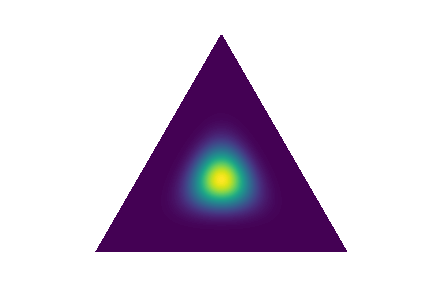
\includegraphics[width=0.3\textwidth]{img/dirichlet101010.png}
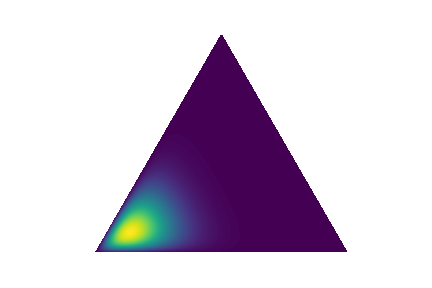
\includegraphics[width=0.3\textwidth]{img/dirichlet1022.png}
\caption{Distribuciones Dirichlet para $k=3$ con parámetros de concentración $\alpha$ (desde izquierda a derecha) dado por $[1,1,1]$, $[10,10,10]$ y $[10,2,2]$. }.
\label{fig:dist_Dirichlet}
\centering
\end{figure}


Veamos a continuación que la distribución de Dirichlet es conjugada al modelo Multinomial, y consecuentemente para Bernoulli, Categórica y Binomial. En efecto, si $\theta \sim \dir{\theta;\alpha}$ y $X\sim\mul{X;n,\theta}$, entonces

\begin{align}
	p(\theta|x) &= \frac{\mul{x;n,\theta}\dir{\theta;\alpha}}{p(x)}\nonumber\\
				&=  \frac{n!}{ x_1!\cdots x_k!p(x) B(\alpha)} \prod_{i=1}^k \theta_i^{x_i + \alpha_i-1}\nonumber\\
				&=  \frac{1}{B(\alpha')} \prod_{i=1}^k \theta_i^{\alpha'_i-1}
				\label{eq:dirichlet_post}
\end{align}
donde $\alpha' = (\alpha'_1,\ldots,\alpha'_k) = (\alpha'_1 + x_1,\ldots,\alpha'_k+ x_k)$ es el nuevo parámetro de concentración.

\begin{example}
	Consideremos $\alpha = [1,2,3,4,5]$ y generemos una muestra de $\theta\sim\dir{\theta|\alpha}$. El siguiente código genera, grafica e imprime esta muestra. 
	\begin{lstlisting}[language=Python]
	import numpy as np
	alpha = np.array([1,2,3,4,5]) 
	theta = np.random.dirichlet(alpha)
	plt.bar(np.arange(5)+1, theta);
	print(f'theta = {theta}')
\end{lstlisting}
En nuestro caso, obtuvimos los parámetros $ \theta = [0.034, 0.171, 0.286, 0.185, 0.324]$.

 Ahora, usaremos un prior Dirichlet sobre $\theta$ con $\alpha_p = [1,1,1,1,1]$ calcularemos la posterior de acuerdo a la ecuación \ref{eq:dirichlet_post}. La Figura \ref{fig:post_Dirichlet} muestra 100 muestras de la distribución posterior para una cantidad de observaciones igual a 

\begin{figure}[H]
\centering
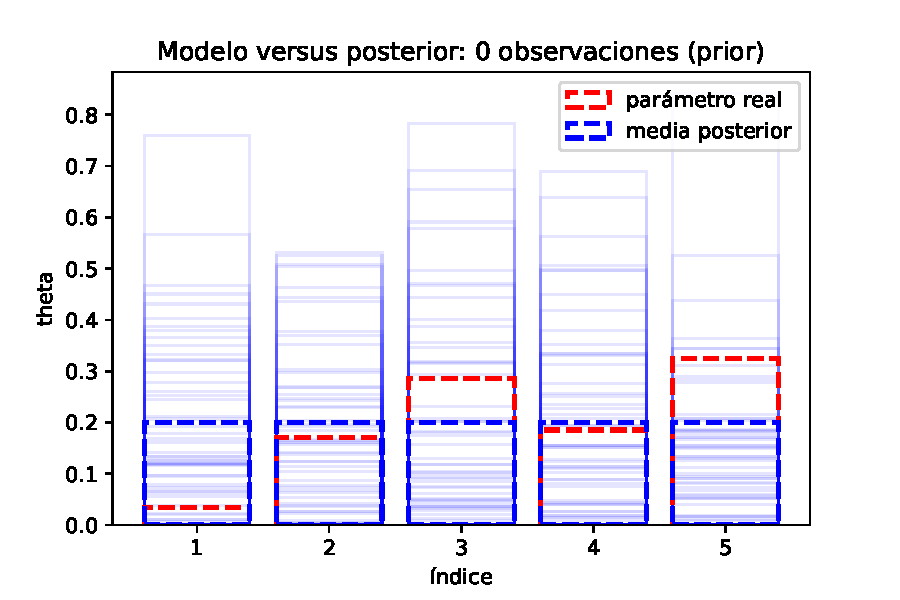
\includegraphics[width=0.3\textwidth]{img/post_dirichlet_0.pdf}
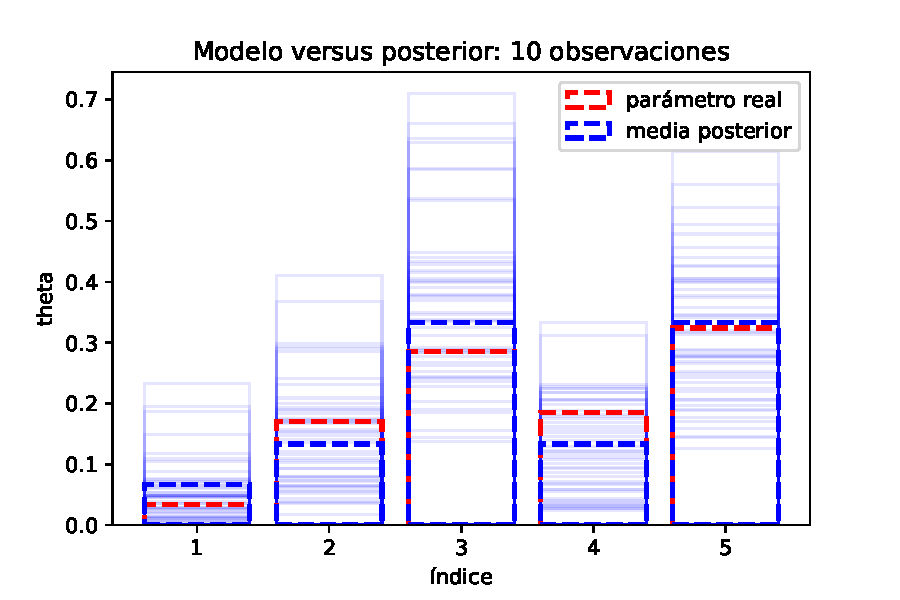
\includegraphics[width=0.3\textwidth]{img/post_dirichlet_10.pdf}
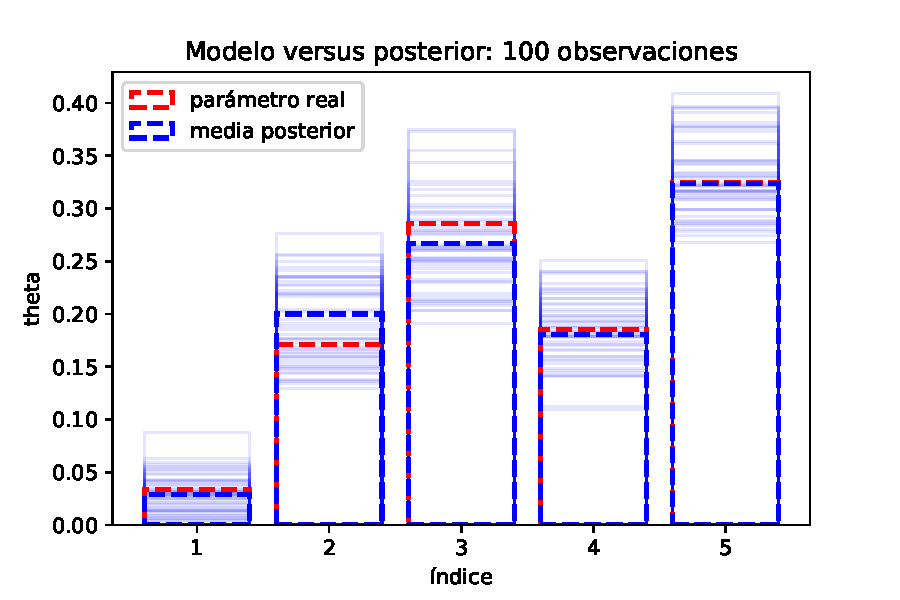
\includegraphics[width=0.3\textwidth]{img/post_dirichlet_100.pdf}\\
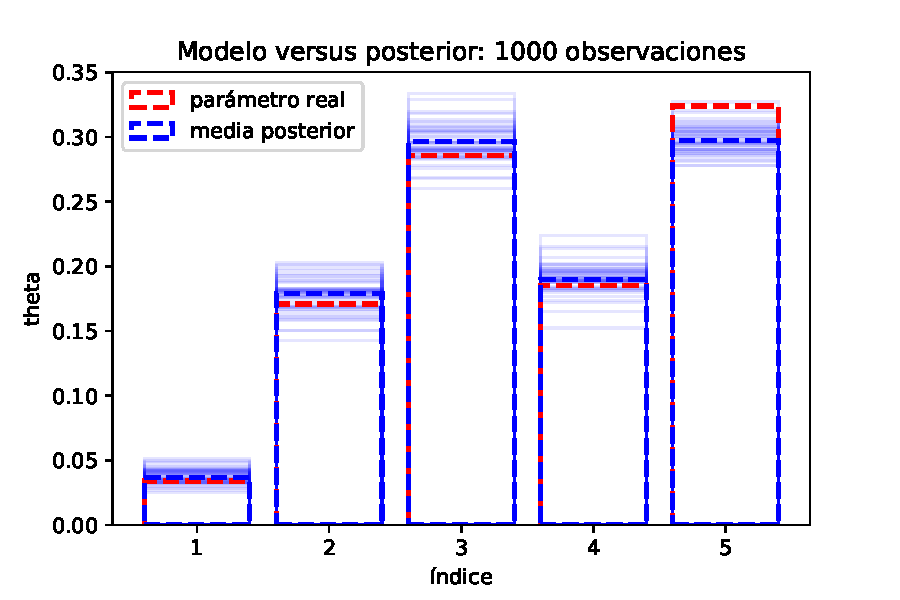
\includegraphics[width=0.3\textwidth]{img/post_dirichlet_1000.pdf}
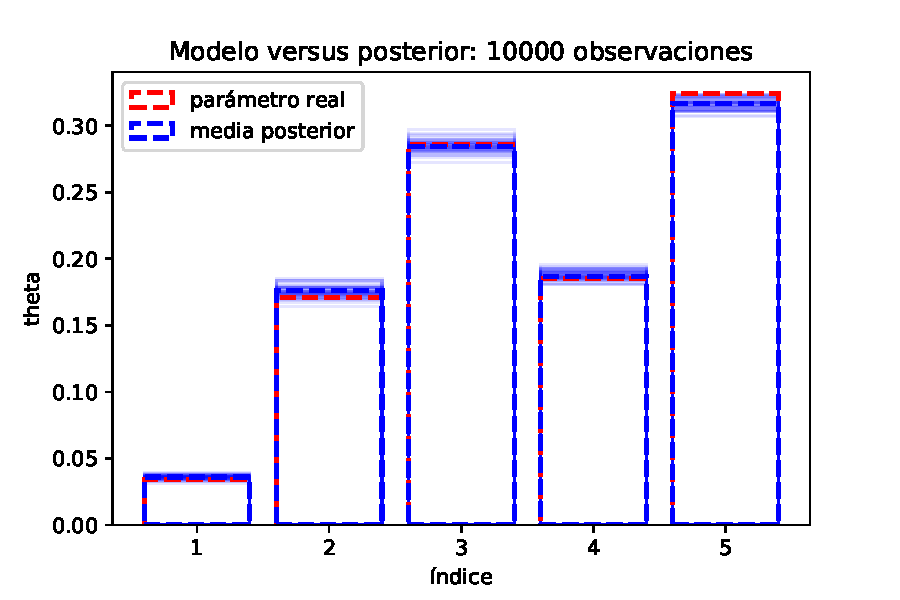
\includegraphics[width=0.3\textwidth]{img/post_dirichlet_10000.pdf}
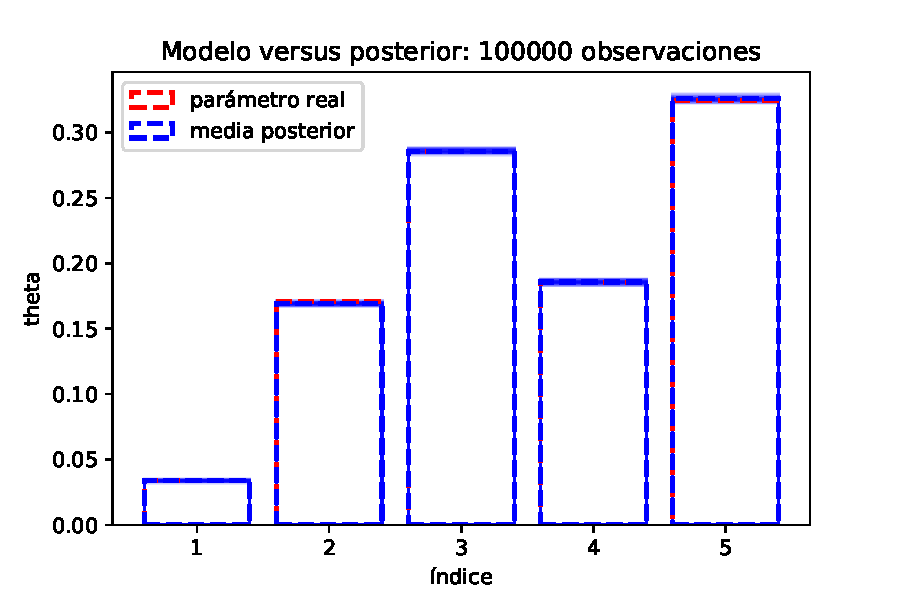
\includegraphics[width=0.3\textwidth]{img/post_dirichlet_100000.pdf}
\caption{Concentración de la distribución posterior en torno al parámetro real para $X\sim\mul{\theta}$ y $\theta\sim\dir{\alpha}$. Se considera desde 0 hasta $10^5$ observaciones y cada gráfico (desde izquierda-arriba hasta derecha-abajo) muestra el parámetro real (linea roja quebrada), la media de la posterior (línea azul quebrada) y 50 muestras de la posterior (azul claro). Observe como la distribución a priori (linea roja quebrada en la primera figura) pierde importancia a medida que el número de observaciones aumenta.}
\label{fig:post_Dirichlet}
\end{figure}
\end{example}

Hay ocasiones en que se busca que la información que hay en los datos es mucho mayor a lo que sabemos de ellos. Para reflejar esta idea, se usan priors impropios.

\begin{definition}[Prior impropia] Una distribución a priori impropia es una distribución que no es necesariamente de probabilidad (i.e., no integra 1), pero que de todas formas puede ser utilizada como distribución a priori en el contexto de inferencia bayesiana, pues la distribución posterior correspondiente si es una distribución de probabilidad apropiada. 
\end{definition}

\begin{remark} Veamos que un prior impropio puede incluso tener integral infinita, en el caso de la distribución normal $X\sim\cN(X;\mu,1)$,  $\mu\in\R$, podemos elegir $p(\mu)\propto1$ y escribir 
\begin{equation}
	p(\mu|x)\propto p(x|\mu)\cdot 1 = \cN(x;\mu,1) = \cN(\mu;x,1). 
\end{equation}
	
\end{remark}

Considerar distribuciones uniformes impropias como priors no informativas parece tener sentido, pues intuitivamente no estamos dando preferencia (mayor probabilidad a priori) a ningún valor del parámetro por sobre otro. Sin embargo, este procedimiento sufre de una desventaja conceptual.

\begin{example} \textbf{Modelo gaussiano ($\sigma^2$ conocido).} Consideremos el prior sobre la media $p(\mu) = \cN(\mu_0,\sigma_0^2)$, con lo que la posterior está dada por  
 \begin{align}
 	p(\mu|\mathcal{D}) &\propto \prod_{i=1}^n \frac{1}{\sqrt{2\pi\sigma^2}}\exp\left(-\frac{1}{2\sigma^2}(x_i-\mu)^2\right) \frac{1}{\sqrt{2\pi\sigma_0^2}}\exp\left(-\frac{1}{2\sigma_0^2}(\mu-\mu_0)^2\right)\label{eq:post_normal_mu_1}\\
 	&\propto \exp\left(-\frac{1}{2\sigma^2}\sum_{i=1}^n(x_i-\mu)^2-\frac{1}{2\sigma_0^2}(\mu-\mu_0)^2\right),\label{eq:post_normal_mu_2}
 \end{align} 
 donde la proporcionalidad viene de ignorar la constante $p(\mathcal{D})$ en la primera línea e ignorar todas las contantes que no dependen de $\mu$ en la segunda línea; recordemos que estas constantes para $\mu$ incluyen a la varianza de $x$, $\sigma^2$, por lo que ignorar esta cantidad es solo posible debido a que estamos considerando el caso en que $\sigma^2$ es conocido. Completando el la forma cuadrática para $\mu$ dentro de la exponencial en la ec.~\eqref{eq:post_normal_mu_2}, obtenemos
 \begin{equation}
 	p(\mu|\mathcal{D}) \propto \exp\left(-\frac{1}{2\sigma_n^2}(\mu - \mu_n)^2\right),\label{eq:post_normal_mu_3}
 \end{equation} 
 donde (ya definiremos $\mu_n$ y $\sigma_n^2$ en breve) como $p(\mu|\mathcal{D})$ debe integrar uno, la única densidad de probabilidad proporcional al lado derecho de la ecuación anterior es la Gaussiana de media $\mu_n$ y varianza $\sigma_n^2$. Es decir, la constante de proporcionalidad necesaria para la igualdad en la expresión anterior es $\int_\R\exp\left(-\frac{1}{2\sigma_n^2}(\mu - \mu_n)^2\right)\d\mu = (2\pi\sigma_n^2)^{n/2}$. Consecuentemente, confirmamos que el prior elegido era efectivamente conjugado con la verosimilitud gaussiana y la posterior está dada por la siguiente gaussiana:
  \begin{equation}
 	p(\mu|\mathcal{D}) = \cN(\mu;\mu_n,\sigma_n^2) = \frac{1}{(2\pi\sigma_n^2)^{N/2}}\exp\left(-\frac{1}{2\sigma_n^2}(\mu - \mu_n)^2\right),\label{eq:post_normal_mu_4}
 \end{equation} 
 donde la media y la varianza están dadas respectivamente  por 
 \begin{align}
 	\mu_n &= \frac{1}{\tfrac{1}{\sigma_0^2} + \tfrac{n}{\sigma^2}} \left(\frac{1}{\sigma_0^2}\mu_0 + \frac{n}{\sigma^2}\bar{x} \right), \quad \text{donde } \bar{x} = \frac{1}{n}\sum_{i=1}^n x_i\label{eq:post_Gm}\\
 	\sigma_n &= \left(\frac{1}{\sigma_0^2} + \frac{n}{\sigma^2}\right)^{-1}.\label{eq:post_Gv}
 \end{align}
\end{example}
\begin{remark}
	La actualización bayesiana transforma los parámetros del prior de  $\mu$ desde  $\mu_0$ y $\sigma_0^2$ hacia $\mu_n$ y $\sigma_n^2$ en las ecs.~\eqref{eq:post_Gm} y \eqref{eq:post_Gv} respectivamente. Notemos que los  parámetros de la posterior son combinaciones (interpretables por lo demás) entre los parámetros del prior y los datos, en efecto, la $\mu_n$ es el promedio ponderado entre  $\mu_0$ (que es nuestro candidato para $\mu$ antes de ver datos) con factor $\sigma_0^{-2}$ y el promedio de los datos $\bar{x}$ con factor $(\sigma^{2}/n)^{-1}$, que a su vez es el estimador de máxima verosimilitud. Es importante también notar que  estos  factores son las varianzas inversas---i.e., precisión---de $\mu_0$ y de $\bar{x}$. Finalmente, observemos que $\sigma_n$ es la \emph{suma paralela} de las varianzas, pues  si expresamos la ec.~\eqref{eq:post_Gv} en términos de \emph{precisiones}, vemos que la precisión inicial $\sigma_0^2$ aumenta un término $\sigma^2$ con cada dato que vemos; lo cual tiene sentido pues con más información es la precisión la que debe aumentar y no la incertidumbre (en este caso representada por la varianza).
\end{remark}
\begin{example} \textbf{Modelo gaussiano ($\mu$ conocido).} Ahora procedemos con el siguiente prior para la varianza, llamado Gamma-inverso:
 \begin{equation}
 	p(\sigma^2)= \text{inv-}\Gamma(\sigma^2;\alpha,\beta) = \frac{\beta^\alpha}{\Gamma(\alpha) (\sigma^2)^{\alpha+1}}\exp(-\beta/\sigma^2)
 \end{equation}
 esta densidad recibe dicho nombre pues es equivalente a modelar la precisión, definida como el recíproco de la varianza $1/\sigma^2$, mediante la distribución Gamma. Los hiperparámetros $\alpha$ y $\beta$ son conocidos como parámetros de forma y de tasa (o precisión) respectivamente. 

 Con este prior, la posterior de la varianza toma la forma:
 \begin{align}
 	p(\sigma^2|\mathcal{D}) &\propto \prod_{i=1}^N \frac{1}{\sqrt{2\pi\sigma^2}}\exp\left(-\frac{1}{2\sigma^2}(x_i-\mu)^2\right) \frac{\beta^\alpha}{\Gamma(\alpha) (\sigma^2)^{\alpha+1}}\exp(-\beta/\sigma^2)\\
 	&\propto  \frac{1}{(\sigma^2)^{N/2+\alpha+1}}\exp\left(-\frac{1}{\sigma^2}\left(\frac{1}{2}\sum_{i=1}^N(x_i-\mu)^2 +\beta\right) \right)\nonumber
 \end{align} 
 donde nuevamente la proporcionalidad ha sido mantenida debido a la remoción de las constantes. Esta última expresión es proporcional a una distribución Gamma inversa con hiperparámetros $\alpha$ y $\beta$ ajustados en base a los datos observados. 


\end{example}


\section{Máxima Verosimilitud} % (fold)
\label{sec:estimador_de_máxima_verosimilitud}

Informalmente, el estimador de un parámetro es una función de los datos que deseamos que entregue un valor cercano al parámetro. Dada una cantidad desconocida, se hace natural la idea de buscar encontrar una "buena" función de los datos que nos permita estimarla, pero ¿Qué significa que un estimador sea un buen estimador? \\
Para comenzar el estudio de los estimadores, debemos definir qué entenderemos formalmente como estimador: 
\begin{definition}
Dadas variables aleatorias $X_1,...,X_n$, con distribución conjunta dada por el parámetro $\theta$ tomando valores en $\R$, un estimador es una función $F(X_1,..X_n)$ a valores reales. 
\end{definition}

\begin{remark}
Un estimador es, por definición, un estadístico. 
\end{remark}

Como ya mencionamos, es natural buscar que el estimador de $\theta$ esté cerca de $\theta$. Dado que $\theta$ es desconocido, es imposible calcular que tan cerca se está de $\theta$ de forma determinista. Sin embargo, si podemos hacerlo desde un enfoque probabilista. \\
Para ver que un estimador $F(X)$ de $\theta$ es cercano a $\theta$, buscaremos que su error $F(X)-\theta$ sea \textbf{probablemente} cercano a 0. \\
Para lo anterior, se hace necesario definir una función que nos permita cuantificar que tan cerca o lejos se está de $\theta$. Teniendo eso en mente, definimos las funciones de pérdida.

En esta sección, veremos cómo construir estimadores usando directamente la densidad de probabilidad de la VA $X\in\cX$, para cual es importante tener en cuenta la definición \ref{función_verosimilitud}. 
El primer estimador que veremos, es el estimador de máxima verosimilitud.

La definición \ref{función_verosimilitud} simplemente establece que la verosimilitud es la distribución (conjunta) de los datos pero donde tomamos los datos como fijos y el parámetro como variable, lo cual tiene sentido en aplicaciones de modelos estadísticos donde los datos son fijos y conocidos pero el modelo (parámetro)
no lo es. Una consecuencia importante de este concepto es que la verosimilitud no es una densidad de probabilidad (en $\theta$) pues no integra 1 (con respecto a $\theta$). Notemos que nos referimos a la \textbf{verosimilitud del parámetro $\theta$} como la densidad de $x$ dado $\theta$ (y no al revés).

La verosimilitud da las condiciones para determinar un estimador que recibe mucha atención en la literatura estadística: 

\begin{definition}[Estimador de máxima verosimilitud (MV)]
	Sea una observación $x$ y una función de verosimilitud $L(\theta)$, el estimador de máxima verosimilitud es 
	\begin{equation}
		\thetaMV = \underset{\theta}{argmin} L(\theta|x)
	\end{equation}	
\end{definition}

Claramente, el estimador de MV puede ser definido con respecto a la verosimilitud o a cualquier función no decreciente de ésta, como también pude no existir o no ser único. En particular, nos enfocaremos en encontrar $\thetaMV$ mediante la maximización de la log-verosimilitud, la cual es usualmente más fácil de optimizar en términos computacionales o analíticos. De hecho, muchas veces incluso ignoraremos constantes de la (log) verosimilitud, pues éstas no cambian el máximo de $L(\theta)$.

\begin{example}[Máxima verosimilitud: Bernoulli]
	\label{ex:bernoulli_MV}
	Sea $X_1,\ldots X_n\sim\ber{\theta}$, la verosimilitud de $\theta$ está dada por 
	\begin{equation}
		L(\theta) = \prod_{i=1}^n\theta^x_i(1-\theta)^{1-x_i}
	\end{equation}
	y su log-verosimilitud por $l(\theta) = (\sum_{i=1}^nx_i)\log \theta + (n-\sum_{i=1}^nx_i)\log(1-\theta)$. El estimador de  MV puede ser encontrado resolviendo $\frac{\partial l(\theta)}{\partial \theta} = 0$:
	\begin{align*}
	\frac{\partial l(\theta)}{\partial \theta} =0 
	&\Rightarrow  (\sum_{i=1}^nx_i) \theta^{-1} = (n-\sum_{i=1}^nx_i)(1-\theta)^{-1}\\
	&\Rightarrow  \sum_{i=1}^nx_i (1-\theta) = (n-\sum_{i=1}^nx_i) \theta\\
	&\Rightarrow  \theta = \sum_{i=1}^nx_i/n.
	\end{align*}
Notemos que este estimador de MV ¡es a su vez el EIVUM!	
\end{example}


\begin{exercise}
	Graficar $l(\theta)$ en el Ejemplo \ref{ex:bernoulli_MV}.
\end{exercise}

\begin{exercise}
	Encuentre el estimador de MV de $\theta = (\mu,\Sigma)$ para la VA $X\sim\cN(\mu,\Sigma)$.
\end{exercise}

\begin{example}
	Sea la VA $X\sim\uni{\theta}$, es decir, $p(x) = \theta^{-1} \ind_{0\leq x \leq \theta}$. Para calcular la verosimilitud, recordemos en primer lugar que la verosimilitud factoriza de acuerdo a  
	\begin{equation}
		L(\theta) = \prod_{i=1}^n p_\theta(x_i)
	\end{equation}
	y observemos que necesariamente $p_\theta(x_i) = 0$ si $x_i>\theta$. Consecuentemente, $L(\theta)>0$ solo si $\theta$ es mayor que toda las observaciones, en particular, si $\theta\geq\max\{x_i\}_1^n$.

	Además, si efectivamente tenemos $\theta\geq\max\{x_i\}_1^n$, entonces notemos que $p_\theta(x_i) = 1/\theta$, por lo que la verosimilitud está dada por
		\begin{equation}
		L(\theta) = \theta^{-n}, \quad \theta\geq\max\{x_i\}_1^n
	\end{equation}
	y consecuentemente, el estimador de máxima verosimilitud es $\thetaMV = \max\{x_i\}_1^n$
\end{example}

\section{Estimador de MV en la práctica: tres ejemplos} % (fold)
\label{sub:MV_tres_ejemplos}

\subsection{Regresión lineal y gaussiana} 
\label{sub:reg_lin}


Una aplicación muy popular del estimador de MV es en los modelos de regresión lineal y gaussianos. Consideremos el caso donde se desea modelar la cantidad de pasajeros que mensualmente viajan en una aerolínea, para esto, sabemos de nuestros colaboradores en la división de análisis de datos de la aerolínea que ésta cantidad tiene una tendencia de crecimiento cuadrática en el tiempo y además una componente oscilatoria de frecuencia anual. Estos fenómenos pueden ser explicados por el aumento de la población, los costos decrecientes de la aerolínea y la estacionalidad anual de las actividades económicas. 

Asumiendo que la naturaleza de la cantidad de pasajeros es estocástica, podemos usar los supuestos anteriores para modelar la densidad condicional  de dicha cantidad (con respecto al tiempo $t$) mediante una densidad normal parametrizada de acuerdo a 
\begin{equation}
	X \sim \cN\left(\theta_0 + \theta_1 t^2 + \theta_2\cos(2\pi t/12), \theta_3^2\right),
\end{equation}
donde $\theta_0,\theta_1,\theta_2$ parametrizan la media y $\theta_3$ la varianza. 

Consecuentemente, si nuestras observaciones están dadas por $\{(t_i,x_i)\}_{i=1}^n$ podemos escribir la log-verosimilitud de $\theta$ como 
\begin{align}
	\label{eq:logV_ejemplo_reg}
	l(\theta) 	&=\loga{\prod_{i=1}^n \frac{1}{\sqrt{2\pi\theta_3^2}}\expo{-\frac{(x_i-\theta_0 - \theta_1 t^2 - \theta_2\cos(2\pi t/12))^2}{2\theta_3^2}}}\nonumber \\
	&=\frac{n}{2}\loga{2\pi\theta_3^2}  - \frac{1}{2\theta_3^2}\sum_{i=1}^n (x_i - \theta_0 - \theta_1 t_i^2 - \theta_2\cos(2\pi t_i/12))^2
\end{align}
con lo que vemos que $\thetaMV$ puede ser calculado explícitamente y es función de $\{(t_i,x_i)\}_{i=1}^n$ debido a que la ecuación \eqref{eq:logV_ejemplo_reg} es cuadrática en $[\theta_0,\theta_1,	\theta_2]$.


% subsection estimador_de_mv_en_la_práctica_tres_ejemplos (end)

\subsection{Regresión no lineal: clasificación} 
\label{sub:clasif}

La razón por la cual $\thetaMV$ pudo ser calculado de forma explícita es porque el modelo Gaussiano con media parametrizada de forma lineal resulta en una log-verosimilitud cuadrática, donde el mínimo es único y explícito. Sin embargo, en muchas situaciones el modelo lineal y gaussiano no es el apropiado. 

Un ejemplo es esto es problema de evaluación crediticia (\textit{credit scoring}) donde en base a un conjunto de \textit{características} que definen a un cliente, un ejecutivo bancario debe evaluar si otorgarle o no el crédito que el cliente solicita. Para tomar esta decisión, el ejecutivo puede revisar la base de datos del banco e identificar los clientes que en el pasado pagaron o no pagaron sus créditos para determinar el perfil del \textit{pagador} y el del \textit{no-pagador}. Finalmente, un nuevo cliente puede ser \textit{clasificado} como pagador/no-pagador en base su similaridad con cada uno de estos grupos. 

Formalmente, denotemos las características del cliente como $t\in\R^N$ y asumamos que el cliente paga su crédito con probabilidad $\sigma(t)$ y no lo paga con probabilidad $1- \sigma(t)$, la función $\sigma(t)$ a definir. Esto es equivalente a construir la VA $X$
\begin{equation}
 	X|t \sim \ber{\sigma(t)}
 \end{equation} 
 donde $X=1$ quiere decir que el cliente paga su crédito y $X=0$ que no. Una elección usual para la función $\sigma(\cdot)$ es la función logística aplicada a una transformación lineal de $t$, es decir, 
 \begin{equation}
 	\Pr{(X=1|t)} = \frac{1}{1+e^{-(\theta_0 + \theta_1 t)	}}.
 \end{equation}
Notemos que este es un clasificador lineal, donde $\theta = [\theta_0, \theta_1]$ define un hiperplano en $\R^N$ en donde los clientes $t\in\{t | 0\leq \theta_0 + \theta_1 t\}$ pagan con probabilidad mayor o igual a 1/2 y el resto con probabilidad menor o igual a 1/2. Esto es conocido como \textbf{regresión logística}. 

Entonces, usando los registros bancarios $\{(x_i,t_i)\}_{i=1}^n$ ¿cuál es el $\theta = [\theta_0, \theta_1]$ de máxima verosimilitud? Para esto notemos que la log-verosimilitud puede ser escrita como 
\begin{align*}
	l(\theta) &= \log \prod_{i=1}^n p(x_i|t) \\
			  &= \sum_{i=1}^n x_i \log \sigma(t) + \left(n-\sum_{i=1}^n x_i\right)\log(1-\sigma(t))\\
			  &= \sum_{i=1}^n x_i \log \frac{1}{1+e^{-(\theta_0 + \theta_1 t)	}} + \left(n-\sum_{i=1}^n x_i\right)\log(1-\frac{1}{1+e^{-(\theta_0 + \theta_1 t)	}})
\end{align*}
Esta expresión no tiene mínimo global y a pesar que podemos calcular su gradiente, no podemos resolver $\partial l(\theta)/\partial \theta =0$ de forma analítica, por lo que debemos usar métodos de descenso de gradiente.  

\subsection{Variables latentes: \textit{Expectation-Maximisation}} 
\label{sub:EM}

En ciertos escenarios es natural asumir que nuestros datos provienen de una mezcla de modelos, por ejemplo, consideremos la distribución de estaturas en una población, podemos naturalmente modelar esto como una mezcla de distribuciones marginales para las estaturas de hombres y mujeres por separado, es decir, 
\begin{equation}
	X\sim p\cN(X|\mu_H,\Sigma_H) + (1-p)\cN(X|\mu_M,\Sigma_M)
\end{equation}
donde la verosimilitud de los parámetros $\theta = [p, \mu_H, \sigma_H,, \mu_M, \sigma_M]$ dado un conjunto de observaciones $\{x_i\}_{i=1}^n$ es
\begin{align*}
	L(\theta) 	&= \prod_{i=1}^n \left( p\cN(X|\mu_H,\Sigma_H) + (1-p)\cN(X|\mu_M,\Sigma_M) \right)\\
				&= \prod_{i=1}^n \left( p\frac{1}{\sqrt{2\pi\Sigma_H^{-1}}}\expo{\frac{-(x_i-\mu_H)^2}{2\Sigma^2_H}} + (1-p)\frac{1}{\sqrt{2\pi\Sigma_M^{-1}}}\expo{\frac{-(x_i-\mu_M)^2}{2\Sigma^2_M}}\right).
\end{align*}
Optimizar esta expresión con respecto a las 5 componentes de $\theta$ es difícil, en particular por la suma en la expresión, lo cual no permite simplificar la expresión mediante la aplicación de $\log(\cdot)$. 

Una interpretación de la diferencia de este modelo con respecto a los anteriores es la introducción implícita de una  \textit{variable latente} que describe de qué gaussiana fue generada cada observación. Si conociésemos esta variable latente, el problema sería dramáticamente más sencillo. En efecto, asumamos que tenemos a nuestra disposición las observaciones $\{z_i\}_{i=1}^n$ de la VA $\{Z_i\}_{i=1}^n$ las cuales denota de qué modelo es generada cada observación, por ejemplo, $Z_i=0$ (cf. $Z_i=1$) denota que el individuo con estatura $X_i$ es hombre (cf.~mujer).
 
En este caso, asumamos por un segundo que estas variables latentes están disponibles y consideremos los \textbf{datos completos} $\{(x_i,z_i)\}_{i=1}^n$ para escribir la función de verosimilitud completa mediante
\begin{align*}
	l(\theta|z_i,x_i) &= \prod_{i=1}^n \cN(X|\mu_H,\Sigma_H)^{z_i} \cN(X|\mu_M,\Sigma_M)^{(1-z_i)}\\
	&\hspace{-3em}= \sum_{i=1}^n \left( z_i\log\frac{1}{\sqrt{2\pi\Sigma_H^{-1}}}\expo{\frac{-(x_i-\mu_H)^2}{2\Sigma^2_H}} + (1-z_i)\log\frac{1}{\sqrt{2\pi\Sigma_M^{-1}}}\expo{\frac{-(x_i-\mu_M)^2}{2\Sigma^2_M}}\right).
\end{align*}
Esta función objetivo es mucho más fácil de optimizar, pero no es observable pues la VA $Z$ es desconocida. Una forma de resolver esto es tomando la esperanza condicional de la expresión anterior (con respecto a $Z$) condicional a los datos y los parámetros \textit{actuales}, para luego maximizar esta expresión c.r.a. $\theta$ y comenzar nuevamente. Específicamente, como la expresión anterior es lineal en $z_i$ basta con tomar su esperanza: 
\begin{align*}
	\Et{Z_i|\theta_t,x_i} &= 1\cdot\Prob{Z_i=1|\theta_t,x_i} + 0\cdot\Prob{Z_i=0|\theta_t,x_i}\\
	&= 	\frac{\Prob{x_i|\theta_t,z_i=1} p(z_i=1)}{p(x_i|\theta)}\\
	&= 	\frac{\Prob{x_i|\theta_t,z_i=1} p(z_i=1)}{p(x_i|z=1,\theta)p(z=1)+p(x_i|z=0	,\theta)p(z=0)}
\end{align*}









\section{Propiedades del EMV} 
\label{sec:propiedades_EMV}
\subsection{Consistencia} 

La primera propiedad que veremos del EMV es su consistencia. Que un estimador sea \textit{consistente} quiere decir que éste tiende (de alguna forma) al parámetro real a medida vamos considerando más datos. Para verificar esto, primero definamos la divergencia de Kullback-Leibler entre las densidades $f$ y $g$ como 
\begin{equation}
	\KL{f}{g} = \int_\cX f(x)\loga{\frac{f(x)}{g(x)}}\dx
\end{equation}
Observemos que la divergencia KL es siempre positiva $\forall f,g$ (desigualdad de Gibbs):
\begin{align*}
 	-\KL{f}{g}  &= \int_\cX f(x)\loga{\frac{g(x)}{f(x)}}\dx\\
 				&\leq \loga{\int_\cX f(x)\frac{g(x)}{f(x)}}\dx, \quad\quad \text{(Jensen's)}\\
 				&= \loga{\int_\cX g(x)}\dx\\
 				&=\log 1=0	
 \end{align*} 
 y como $\log$ es estrictamente convexo, la igualdad solo se cumple si el argumento $\frac{g(x)}{f(x)}$ es constante, lo cual se tiene solo para ${g(x)} = {f(x)}$.

 Otra propiedad clave de la divergencia KL es que puede ser infinita y es asimétrica. La intuición detrás de la KL es que es una medida de \textit{error} de estimar una distribución con respecto a la otra. 

 Con la KL, definiremos que un modelo/parámetro es \textbf{identificable} si los valores para los parámetros $\theta\neq\theta'$ implican $\KL{p_\theta}{p\theta'}>0$ lo que significa que distintos valores del parámetro dan origen a distintos modelos---asumiremos desde ahora que los modelos considerados son identificables.

Observemos que el estimador de MV puede ser obtenido de la maximización de

\begin{equation}
 	M_n (\theta') = n^{-1} (l_n(\theta') - l_n(\theta))  = \frac{1}{n} \sum_{i=1}^n \loga{\frac{p_{\theta'}(x_i)}{p_{\theta}(x_i)}}
 \end{equation} 
 donde $n$ es la cantidad de observaciones $x_1,\ldots,x_n$, $\theta$ es el parámetro real y $l_n(\cdot)$ es la log-verosimilitud. Esto es posible porque $l_n(\theta)$ es constante para $\theta'$. Veamos que gracias a la ley de los grandes números, tenemos que 
 \begin{equation}
 	M_n(\theta') \rightarrow \Et{\loga{\frac{p_{\theta'}(x)}{p_{\theta}(x)}}} = -\Et{\loga{\frac{p_{\theta}(x)}{p_{\theta'}(x)}}} = -\KL{p_\theta}{p_{\theta'}}
 \end{equation}

 Consecuentemente, como el objetivo del estimador de MV tiende a la KL negativa, entonces maximizar la verosimilitud es equivalente a minimizar la KL-divergencia entre el modelo real y el modelo generado por el parámetro. Si el modelo generado tiende al modelo real, nuestro supuesto de \textit{identificabilidad} implica que el estimador de MV tiene al parámetro real. 

 Otra propiedad muy utilizada en la práctica es el \textbf{Principio de equivarianza}, el cual establece que si $\thetaMV$ es el estimador de MV de $\theta$, entonces, $g(\thetaMV)$ es el estimador de MV del parámetro transformado $g(\theta)$.

\begin{example}(Cálculo del EMV en Gaussiana: varianza versus precisión versus log-precisión versus cholesky - reparametrisation trick)
	
\end{example}

\subsection{Normalidad asintótica}

Otra propiedad es la \textbf{normalidad asintótica del EMV}, esto significa que la distribución del estimador ML (como cantidad aleatoria) es normal a medida se incluyen más observaciones. Para estudiar esta propiedad, primero definamos la función de puntaje o \textit{score function} como \textbf{función aleatoria }definida por la derivada de la log-verosimilitud, es decir, 
\begin{equation}
	S_\theta(X) = \frac{\partial \log p_\theta(X)}{\partial\theta}.
\end{equation}
Observemos que la esperanza de la función de puntaje cero. En efecto, derivando la igualdad fundamental $1 = \int_\cX p_\theta(x)\dx$ con respecto a $\theta$, obtenemos 
\begin{align}
	0 = \int_\cX \frac{\partial  p_\theta(X)}{\partial\theta} \dx = \int_\cX \frac{1}{p_\theta(X)}\frac{\partial  p_\theta(X)}{\partial\theta} p_\theta(X) \dx = \int_\cX \frac{\partial \log   p_\theta(X)}{\partial\theta} p_\theta(X) \dx = \Et{S_\theta(X)}
\end{align}
Sorprendente. 

Ahora, derivemos una vez más con lo cual obtenemos: 
\begin{align*}
	0 &= \int_\cX \frac{\partial}{\partial \theta }\left(\frac{\partial \log   p_\theta(X)}{\partial\theta} p_\theta(X) \right)\dx\\ 
	&= \int_\cX \left(\frac{\partial^2 \log   p_\theta(X)}{\partial\theta^2} p_\theta(X) + \frac{\partial \log   p_\theta(X)}{\partial\theta}\frac{\partial   p_\theta(X)}{\partial\theta}  \right)\dx\\
	&= \Et{\frac{\partial^2 \log   p_\theta(X)}{\partial\theta^2}} + \Et{\left(\frac{\partial \log   p_\theta(X)}{\partial\theta}\right)^2}
\end{align*}
donde podemos observar que cada una de estos términos tiene la misma magnitud (uno es negativo y el otro es positivo). Esta magnitud es conocida como \textit{información de Fisher}, denotada como 
\begin{equation}
		I(\theta) = \Et{\left(\frac{\partial \log   p_\theta(X)}{\partial\theta}\right)^2} = 	-\Et{\frac{\partial^2 \log   p_\theta(X)}{\partial\theta^2}}.
\end{equation}	
Recordemos además que como la esperanza de la función de puntaje es nulo, entonces, su varianza puede ser expresada como 
\begin{equation}
	\Vt{S_\theta(X)} = \Et{S_\theta(X)^2} - \cancel{\Et{S_\theta(X)}^2} = \Et{\left(\frac{\partial \log   p_\theta(X)}{\partial\theta}\right)^2}
\end{equation}
consecuentemente, la información de Fisher también es la varianza de la función de pérdida. Ya contamos con tres expresiones para poder calcular esta cantidad. 

\begin{exercise}[Cálculo de la información de Fisher para Bernoulli]
	Consideremos $X\sim\ber{\theta}$, entonces, 
	\begin{align}
		I(\theta) &= -\Et{\frac{\partial^2}{\partial\theta^2}\loga{\theta^X(1-\theta)^{1-X}}}\nonumber\\
		&= -\Et{\frac{\partial^2}{\partial\theta^2} X\log\theta + \frac{\partial^2}{\partial\theta^2} 	(1-X)\loga{1-\theta}	}\nonumber\\
		&= \Et{X\theta^{-2} + (1-X)(1-\theta)^{-2}	}\nonumber\\
		&= \theta^{-1} + (1-\theta)^{-1}	\nonumber\\
		&= 	\frac{1}{\theta(1-\theta)}	
	\end{align}
\end{exercise}

\begin{exercise}[Cálculo de la información de Fisher para Poisson]
	Consideremos $X\sim\poi{\theta}$, entonces, 
	\begin{align}
		I(\theta) &= \Et{\left(\frac{\partial}{\partial\theta}\loga{\frac{\theta^Xe^{-\theta}}{X!}}\right)^2}\nonumber	\\
		&= \Et{\left( \frac{\partial}{\partial\theta}X\log\theta - \frac{\partial}{\partial\theta}\theta - \frac{\partial}{\partial\theta}\log(X!)\right)^2}\nonumber\\
		&= \Et{\left( X\theta^{-1} - 1\right)^2}\nonumber	\\
		&= \Et{ X^2\theta^{-2} -2X\theta^{-1}+ 1}\nonumber	\\
		&= (\theta+\theta^2)\theta^{-2} -2\theta\theta^{-1}+ 1\nonumber\\
		&= \theta^{-1}\nonumber	
	\end{align}
\end{exercise}

El cálculo anterior ha sido para la verosimilitud en base a una variable aleatoria, si consideramos la verosimilitud evaluada calculada para un conjunto de observaciones (IID), tenemos que

\begin{equation}
	S_\theta(X_1,\ldots,X_n) = \frac{\partial \log \prod_{i=1}^np_\theta(X_i)}{\partial\theta} = \sum_{i=1}^n\frac{\partial \log p_\theta(X_i)}{\partial\theta}= \sum_{i=1}^n S_\theta(X_i)
\end{equation}
y de igual forma para la información de Fisher, tenemos, 

\begin{equation}
	I_n(\theta) = \Vt{\sum_{i=1}^n S_\theta(X_i)} = n I(\theta)
\end{equation}

Veamos ahora una desigualdad interesante para la información de Fisher y su relación con estimadores. Consideremos un estimador insesgado, es decir, 
\begin{equation}
	\Et{\hat{\theta}(X)-\theta}=\int_\cX (\hat{\theta}(X)-\theta)p_\theta(X)\dx=0.
\end{equation}
Derivando esta expresión con respecto a $\theta$, obtenemos

\begin{align*}
	0 &= \frac{\partial}{\partial\theta}\int_\cX (\hat{\theta}(X)-\theta)p_\theta(X)\dx\\
	  &= -\int_\cX p_\theta(X)\dx  + \int_\cX (\hat{\theta}(X)-\theta)\frac{\partial p_\theta(X)}{\partial\theta}\dx\\
	  &= -1  + \int_\cX (\hat{\theta}(X)-\theta)\frac{\partial\log p_\theta(X) }{\partial\theta}p_\theta(X)\dx.
\end{align*}
Lo que implica que 
\begin{align*}
	1 &= \left(\int_\cX (\hat{\theta}(X)-\theta)\frac{\partial\log p_\theta(X) }{\partial\theta}p_\theta(X)\dx\right)^2\\
	&=\left(\int_\cX (\hat{\theta}(X)-\theta)\sqrt{p_\theta(X)}\sqrt{p_\theta(X)}\frac{\partial\log p_\theta(X) }{\partial\theta}\dx\right)^2\\
	&\leq\int_\cX (\hat{\theta}(X)-\theta)^2 p_\theta(X)\dx \int\left(\frac{\partial\log p_\theta(X) }{\partial\theta}\right)^2 p_\theta(X)\dx.
\end{align*}
Notemos que la primera integral es la varianza del estimador insesgado $\hat\theta$ y la segunda es la esperanza del cuadrado de la función de puntaje (o la información de Fisher). Con esto, podemos enunciar el siguiente resultado 
\begin{definition}[Cota de Cramer-Rao]
	Sea $X_1,\ldots,X_n \sim p_\theta$ y $nI(\theta)$ su información de Fisher. Entonces para todo estimador insesgado $\theta'$ tenemos 
	\begin{equation}
		\Vt{\theta'}\geq (nI(\theta))^{-1},\quad \forall \theta\in\Theta
	\end{equation}
\end{definition}
La cota de Cramer-Rao es un elemento fundamental en el estudio estadístico, pues establece que cualquier estimador tiene necesariamente una varianza que está por sobre el recíproco de la información de Fisher. 

Ahora podemos finalmente volver al concepto de normalidad asintótica. Si tenemos una colección de VA $X_1,\ldots,X_n\sim p_\theta$ con $\theta$ el parámetro real, entonces, la secuencia de estimadores de MV, $\thetaMV^{(n)}$ cumple con 
\begin{equation}
	\sqrt{n}(\thetaMV^{(n)}-\theta)\rightarrow \cN(0,I(\theta)^{-1})
\end{equation}
lo cual intuitivamente corresponde a que, para $n$ suficientemente grande, el estimador de MV está distribuido de forma normal en torno al parámetro real con varianza $(nI(\theta))^{-1}$. Lo cual implica también \textit{eficiencia asintótica}.

Este resultado es fundamental en estadística aplicada: no importa cómo ha sido obtenido el estimador de MV, si $n$ es suficientemente grande, entonces la distribución del estimador es normal y su varianza tiende a cero. 

\section{Estimadores Bayesianos}



\begin{definition}[Estimador Bayesiano]
Sea $X$ una varible aleatoria. Para cada valor $x$ de $X$, sea $f^{*}(x)$ el valor que minimiza $\mathbb{E}[L(\theta,a)|x]$. Entonces $f^{*}(x)$ es el estimador bayesiano de $\theta$.
\end{definition}

\begin{remark}
\begin{enumerate}
    \item El problema de minimización de $\mathbb{E}[L(\theta,a)|x]$ corresponde a buscar el $\theta \in \Omega$ tal que $\theta$ sea el parámetro que tenga mayores probabilidades de haber generado la muestra de datos, dadas las observaciones y con una función de pérdida dada. 
    \item Estamos tomando en cuenta las observaciones que hemos visto \textbf{y} el conocimiento previo, expresado en nuestro prior. Esto nos dá la oportunidad de introducir sesgos expertos al modelo.
    \end{enumerate}
\end{remark}

De ahora en adelante, usaremos la función de mínimos cuadrados como función de pérdida. Teniendo esto en cuenta, procedemos a definir el siguiente estimador bayesiano: 

\begin{definition}{Máximo a posteriori}
Sea $\theta \in \Theta$ un parámetro con distribución a posteriori $p(\theta |D)$ definida en todo $\Theta$. Entonces nos referiremos a su estimación puntual dada por: 
$$
\theta_{MAP}= \underset{\Theta}{argmax} p(\theta|D)
$$
como \emph{máximo a posteriori} (MAP). 
\end{definition}

Notemos que es posible encontrar el MAP incluso cuando solo tenemos acceso a una versión \emph{proporcional} a la distribución posterior, un escenario usual en inferencia bayesiana, o también mediante la maximización del logaritmo de ésta última. En efecto, 
$$
\theta_{MAP} = \underset{\theta \in \Theta}{argmax }p(\theta|\mathcal{D}) = \underset{\theta \in \Theta}{argmax }p(\mathcal{D}|\theta)p(\theta)= \underset{\theta \in \Theta}{argmax }\left(\underbrace{\log p(\mathcal{D}|\theta)}_{l(\theta)} + \log p(\theta)\right),
$$

donde  nuevamente vemos la maximización de  la función de log-verosimilitud, pero ahora junto al log-prior.

\begin{example}[Máximo a posterior para el modelo gaussiano]
En particular, para el modelo lineal y gaussiano que hemos considerado hasta ahora, podemos calcular $\theta_{MAP}$ para un prior Gaussiano de media cero y varianza $\sigma_\theta^2$. Éste está dado por (asumimos la varianza del ruido $\sigma_\epsilon^2$ conocida):	
\begin{align}
	\theta_\text{MAP}^\star 	&= \text{argmax } p(Y|\theta,X)p(\theta)\nonumber\\
	\text{[independencia, definición]}\ &= \text{argmax } \prod_{i=1}^N \cN(y_i;\theta^\top x_i,\sigma_\epsilon^2)\cN(\theta;0,\sigma_\theta^2) \nonumber\\
	&= \text{argmax } \prod_{i=1}^N \frac{1}{\sqrt{2\pi}\sigma_\epsilon} \exp\left({\frac{-1}{2\sigma_\epsilon^2}(y_i-\theta^\top x_i)^2}\right)											\frac{1}{(\sqrt{2\pi}\sigma_\theta)^{M+1}} \exp\left({\frac{-||\theta||^2}{2\sigma_\theta^2}}\right) \nonumber\\
	\text{[reordenar]}  &= \text{argmax } \frac{1}{\sqrt{2\pi}\sigma_\epsilon} \frac{1}{(\sqrt{2\pi}\sigma_\theta)^{M+1}} \exp\left( \sum_{i=1}^N{\frac{-1}{2\sigma_\epsilon^2}(y_i-\theta^\top x_i)^2} -{\frac{||\theta||^2}{2\sigma_\theta^2}}\right) \nonumber\\
	\text{[logaritmo]}\  &= \text{argmin } \sum_{i=1}^N{(y_i-\theta^\to x_i)^2} +{\frac{\sigma_\epsilon^2}{\sigma_\theta^2}||\theta |^2}.\nonumber 
	\label{eq:MAP_reg_lin}
\end{align}
\end{example}




\section{El prior de Jeffreys}

Consideremos $X\sim p(x|\theta)$, $\theta \in [a,b]$, en donde elegimos el prior \textit{no informativo} uniforme dado por 
$$
	p(\theta) =\uni{a,b} = \frac{1}{b-a}.
$$
Consideremos ahora un modelo \textit{reparametrizado} $\eta = e^\theta\in[c,d]$, donde el modelo es expresado como $X\sim q(x|\eta) = p(x|\theta) $. El prior uniforme para el nuevo parámetro es
\begin{equation}
	p(\eta) =\uni{c,d} = \frac{1}{d-c}.
\end{equation}
Observemos que la elección uniforme del parámetro $\theta$ en el intervalo $[a,b]$ es equivalente a elegir $\eta$ según
\begin{equation}
	\tilde{p}(\eta) = p(\theta) \left|\frac{d\theta}{d\eta}\right| = \frac{1}{b-a}\left|\frac{d\log\eta}{d\eta}\right|= \frac{1}{\eta (b-a)},
\end{equation}
es decir, la distribución sobre $\eta$ inducida por $p(\theta)$. Esta distribución por supuesto no es equivalente a elegir $\eta$ uniformemente en el intervalo $[c,d]$. 

Una forma de construir un prior que es invariante ante reparametrizaciones es mediante la metodología propuesta por  Harold Jeffreys (1946), el que sugiere elegir un prior proporcional a la raíz cuadrada del determinante de la información de Fisher, es decir,  
\begin{equation}
	p(\theta) \propto \left( \det I(\theta)\right)^{1/2},
\end{equation}
donde recordemos que la información de Fisher está dada por 
\begin{equation}
	I(\theta) = -\Et{\frac{\partial^2}{\partial\theta^2}\log p(X|\theta)} = \Et{\left(\frac{\partial}{\partial\theta}\log p(X|\theta)\right)^2}.
\end{equation}
Además, si $X_1,\ldots,X_n$ son iid, entonces $I(\theta) = n I_1(\theta)$ y el prior de Jeffreys puede ser expresado como 
\begin{equation}
	p(\theta) \propto  I_1(\theta)^{1/2}.
\end{equation}
Observemos que si $\int_\Omega\sqrt{I(\theta)}\d\theta$ es finito, entonces la constante de proporcionalidad es precisamente esta cantidad. Sin embargo, si esta cantidad es infinita el prior de Jeffreys aún es un prior válido pero impropio, siempre y cuando las posteriores respectivas sí sean propias. 

Veamos ahora que el prior de Jeffreys es invariante bajo reparametrizaciones. Consideremos los modelos relacionados mediante reparametrización dados por 
\begin{equation}
	X\sim p(x|\theta),\ \theta\in\Omega\quad \& \quad X\sim q(x|\eta),\ \eta\in\Gamma,
\end{equation}
donde $\eta = h(\theta)$. Las informaciones de Fisher para ambos modelos, denotadas respectivamente $I_p(\theta)$ e $I_q(\theta)$, están relacionadas mediante
\begin{align}
	I_p(\theta) &= \int_\cX\left(\frac{\partial}{\partial\theta}\log p(x|\theta)\right)^2p(x|\theta)\d x\nonumber\\
				&= \int_\cX\left(\frac{\partial}{\partial\theta}\log q(x|h(\theta))\right)^2q(x|h(\theta))\d x\nonumber\\
				&= \int_\cX\left(\frac{\partial}{\partial\eta}\log q(x|\eta) h'(\theta)\right)^2q(x|\eta)\d x\nonumber\\
				&= \left(h'(\theta)\right)^2 I_q(\eta).
\end{align} 

Observemos ahora que el prior en $\theta$, $p(\theta)$, inducido por el prior de Jeffreys en $\eta$, $p_J(\eta)$, es efectivamente el prior de Jeffreys en $\theta$, $p_J(\theta)$. En efecto, debido al cambio de variable tenemos

\begin{equation}
	p(\theta) = p_J(\eta) \left|\frac{d \eta}{d \theta}\right| = \sqrt{I_q(\eta)}\left|h'(\theta)\right| = \sqrt{I_p(\theta)} = p_J(\theta).
\end{equation}

Como ya mencionamos, la construcción del Prior de Jeffreys surge con la idea de usar un prior que sea invariante bajo transformaciones monótonas y que sea no informativo. ¿Pero cómo se logra esto últmo? Resulta ser que el prior de Jeffreys es el prior uniforme sobre el espacio de parámetros $\Theta$, pero no con la métrica euclidiana. La topología que se debe considerar es aquella que calcula la distancia entre dos 
parámetros $\theta_1$ y $\theta_2$ como la distancia de Kulback-Liebler entre sus distribuciones asociadas $f(x|\theta_1)$ y $f(x|\theta_2)$.
Bajo esta métrica, el prior de Jeffreys sigue siendo invariante bajo transformaciones monótonas.
%!TEX root = apunte_estadistica.tex


\chapter{Más Sobre Estimadores}

\section{Intervalos de Confianza} 

En muchas aplicaciones, no es suficiente reportar una estimación puntual, es decir, un valor único para le parámetro a estimar, sino que debe identificarse una rango donde, con cierta probabilidad, el parámetro real está contenido. Esto motiva la siguiente definición: 

\begin{definition}[Intervalo de confianza]
\label{def:conf_inter} Un $(1-\alpha)$-intervalo de confianza para el parámetro $\theta$, $\alpha\in[0,1]$, es el intervalo aleatorio $(A(X),B(X))$ tal que 
\begin{equation}
	\label{eq:conf_inter}
	\Probt{A(X)\leq\theta\leq B(X)} = 1-\alpha, \forall \theta\in\Theta.
\end{equation}
\end{definition}

\begin{remark}
	Es importante notara que la definición arriba no es un enunciado de probabilidad en $\theta$, o en otras palabras, no describe una probabilidad sobre el parámetro $\theta$; pues recordemos que éste es fijo. Por el contrario, lo que es aleatorio en la ecuación \eqref{eq:conf_inter} es el intervalo, no el parámetros. Entonces, si bien es una sutileza, la definición anterior se debe entender como la probabilidad de que ``el intervalo (aleatorio) contenga al parámetro (fijo)'', y no como la probabilidad de que `el parámetro esté en el intervalo'. 
\end{remark}
Una consecuencia clave de este concepto es que si $I_{1-\alpha}$ es un $(1-\alpha)$-intervalo de confianza, entonces si fuese posible repetir una gran cantidad de veces el ejercicio de recolectar datos $X$ y calcular este intervalo para cada una de estas observaciones, entonces el parámetro $\theta$ estaría contenido en le intervalo un $(1-\alpha)\%$. Esto es muy diferente de asegurar que para un solo experimento, la probabilidad de que el parámetro $\theta$ esté contenido en $I_{1-\alpha}$ es $1-\alpha$, lo cual no es cierto. Los siguientes ejemplos tienen por objetivo ayudar a aclarar este concepto.

\begin{example}[Intervalo de confianza para la media de la distribución normal]
	Consideremos la muestra $X_1,\ldots,X_\nu\sim\cN(\theta,1)$. Como $\bar{X}=\frac{1}{n}\sum_{i=1}^nX_i\sim\cN(\theta,1/n)$ tenemos que  
	\begin{equation}
			\sqrt{n}(\bar{X}-\theta)\sim\cN(0,1).
		\end{equation}	
	Esta cantidad se llama \emph{pivote} y es una función (de la VA y del parámetro) cuya distribución no depende del parámetro. Consecuentemente, podemos identificar directamente un intervalo de confianza para el pivote desde una tabla de valores para la distribución normal de media cero y varianza unitaria. Si $\phi(x)$ denota la distribución Normal, entonces podemos elegir  $x_1$ y $x_2$ tal que $\phi(x_2)-\phi(x_1) = 1-\alpha$ con lo que tenemos
	\begin{equation}
	 	\Probt{x_1 \leq \sqrt{n}(\theta-\bar{X}) \leq x_2} = 1-\alpha \Leftrightarrow \Probt{\bar{X} + x_1/\sqrt{n} \leq \theta \leq \bar{X} + x_2/\sqrt{n}} = 1-\alpha,
	 \end{equation} 
	 es. decir, $(\bar{X} + x_1/\sqrt{n},\bar{X} + x_2/\sqrt{n})$ es el $(1-\alpha)$-intervalo de confianza de $\theta$. Eligiendo $\alpha=0.05$ tenemos $x_2 = -x_1 =1.96$ con lo que el intervalo de confianza del 95\% para $\theta$ está dado por 
	 \begin{equation}
	 	(\bar{X} -1.96/\sqrt{n},\bar{X} + 1.96/\sqrt{n}).
	 \end{equation}

	 El procedimiento estándar para encontrar intervalos de confianza es como el ilustrado en el ejemplo anterior, en donde construimos una cantidad que tiene una distribución que no depende del parámetro desconocido (llamada pivote). Construir un intervalo de confianza para esta cantidad es directo desde las tablas de distribuciones, luego, podemos encontrar el intervalo de confianza para la cantidad deseada, e.g., el parámetro desconocido, mediante transformaciones de la expresión del pivote. 

	 \begin{remark}
	 	El intervalo de confianza no es único. Por ejemplo, en el caso gaussiano podemos elegir en intervalo centrado en cero o desde $-\infty$. Esta elección dependerá de las aplicación en cuestión: una regla general es elegirlo de forma centrada para densidades que son simétricas, centrado en la moda para distribuciones unimodales, mientas que para densidades con soporte positivo podemos elegirlo desde cero. 
	 \end{remark}

	 Hasta ahora hemos solo definido intervalos de confianza para cantidades escalares, en donde el concepto de intervalo tiene sentido. Para parámetros vectoriales, nos referiremos a  \textit{conjuntos de confianza}. Siguiendo la Definición \ref{def:conf_inter}, un $(1-\alpha)$-conjunto de confianza $S(X)$ es tal que 
	 \begin{equation}
	\label{eq:conf_set}
	\Probt{\theta\in S(X)} = 1-\alpha, \forall \theta\in\Theta.
\end{equation}
\end{example}


\begin{exercise}
Considere $X_1,\ldots,X_{50}\sim\cN(0,\sigma^2)$, calcule el intervalo de confianza del 99\%.
\end{exercise}

\begin{example}[Intervalo de confianza para Bernoulli] Consideremos $X_1,\ldots,X_{n}\sim\ber{\theta}$ y calculemos un intervalo de confianza para $\theta$. Recordemos que el EMV es $\thetahat = \frac{1}{n}\sum_{i=1}^nX_i$ y debido a la normalidad asintótica del EMV, tenemos que para $n$ grande, podemos asumir 
\begin{equation}
	\thetahat\sim\cN\left(\theta,\frac{\theta(1-\theta)}{n}\right)
\end{equation}
donde la varianza $\frac{\theta(1-\theta)}{n}=I_n(\theta)^{-1}$ es la inversa de la información de Fisher. 

Podemos entonces considerar el pivote
\begin{equation}
	\frac{\sqrt{n}(\thetahat-\theta)}{\sqrt{\theta(1-\theta)}}\sim\cN(0,1)
\end{equation}
y calcular el $(1-\alpha)$-intervalo de confianza asumiendo los valores $x_1$ y $x_2$ mediante 
\begin{align*}
	\Probt{x_1 \leq \tfrac{\sqrt{n}(\theta-\thetahat)}{\sqrt{\theta(1-\theta)}} \leq x_2} = 1-\alpha \Leftrightarrow \Probt{\thetahat + \tfrac{x_1\sqrt{\theta(1-\theta)}}{\sqrt{n}} \leq \theta \leq \thetahat + \tfrac{x_2\sqrt{\theta(1-\theta)}}{\sqrt{n}}} = 1-\alpha.
\end{align*}
Sin embargo, los bordes de este intervalo no son conocidos, pues dependen de $\theta$. Una forma de aproximar el intervalo es reemplazar el parámetro por su EMV. 
\end{example}


\begin{exercise}[Encuesta de elecciones presidenciales] Considere una encuesta que ha consultado a 1000 votantes y su candidato ha recibido 200 votos. Use el resultado del ejemplo anterior para determinar el intervalo de confianza del 95\% de la cantidad de votos que su candidato obtendría en la elección presidencial. 
\end{exercise}

Finalmente, revisaremos el siguiente ejemplo, el cual pretende ejemplificar el concepto de que en solo un experimento, la determinación del $(1-\alpha)$-intervalo de confianza no quiere decir que la probabilidad de que el parámetro esté contenido en él es $(1-\alpha)$\%. 

\begin{example}[Intervalo de confianza para una distribución uniforme] Considere $X_1,X_2\sim\uni{\theta-\tfrac{1}{2},\theta+\tfrac{1}{2}}$ y observe que 
\begin{align*}
	\Probt{\min(X_1,X_2) \leq \theta \leq \max(X_1,X_2)} 
		&= \Probt{ X_1 \leq \theta \leq X_2}  + \Probt{ X_2 \leq \theta \leq X_1} \\
		&= \frac{1}{2}\times \frac{1}{2} + \frac{1}{2}\times\frac{1}{2}\\
		&= \frac{1}{2}
\end{align*}
corresponde al intervalo del 50\%. 

Sin embargo, si observáramos $X_1 = x_1$ y $X_2 = x_2$ tal que $|x_1-x_2|\geq\tfrac{1}{2}$ entonces necesariamente está contenido en el intervalo $(\min(X_1,X_2) , \max(X_1,X_2))$ con probabilidad 1. Esto ilustra la idea de que, en un experimento dado, la probabilidad de que $\theta$ esté en intervalo de confianza del $(1-\alpha)$\% no es necesariamente $(1-\alpha)$\%.
\end{example}

\section{Intervalos de Confianza Bayesianos}
El paradigma bayesiano propone una noción de intervalos de confianza más natural que el enfoque frecuentista, dado que la notación $\mathbb{P}(\theta \in C_x)$ tiene un significado, incluso condicional a $x$.
\begin{definition}
Para un prior $\pi$, un conjunto $C_x$ se dice  $\alpha$-creíble si :
$$
\mathbb{P}^{\pi}(\theta \in C_x |x) \geq 1- \alpha,
$$
para la probabilidad dada por el prior $\pi$. Esta región se dice de Alta Densidad Posterior (HPD por su sigla en inglés) si se puede escribir como:
$$
\left \{\theta: \pi(\theta|x) > k_{\alpha} \right \} \subset C_{x}^{\pi} \subset \left \{ \theta: \pi(\theta|x) \geq  k_{\alpha}\right \} ,
$$
donde $k_{\alpha}$ es la cota más grande tal que: 
$$
\mathbb{P}^{\pi}(\theta \in C_{k}^{\pi}|x) \geq 1- \alpha
$$
\end{definition}
\begin{remark}
    El hecho de considerar regiones HPD viene de que minimizan el volumen entre las regiones $\alpha$-creíbles. 
\end{remark}

\begin{example}
Si $\theta \sim \mathcal{N}(0,\tau^{2})$, la posterior de $\theta$ es una normal $\mathcal{N}(\mu(x),\omega^{-2})$, con $\omega^{2}= \tau^{-2} + \sigma^{-2} $
y $\mu(x)=\dfrac{\tau^{2}x}{\tau^2 + \sigma^2}$. Luego: 
$$
C_{\alpha}^{\pi} =[\mu(x) - k_{\alpha}\omega^{-1},\mu(x)+k_{\alpha}\omega^{-1} ]
$$
con $k_{\alpha}$ el $\alpha /2 $-intil de $\mathcal{N}(0,1)$. En particular, si $\tau \to \infty$, $\pi(\theta)$ converge a la medida de Lebesgue en $\R $ y: 
$$
C_{\alpha}= [x - k_{\alpha}\sigma ,x + k_{\alpha}\sigma],
$$
que corresponde al intervalo de confianza clásico para una normal. 
\end{example}
\chapter{Test de Hipótesis}


\section{Teoría de decisiones}
\label{sec:teoría_de_decisiones}

En términos generales, la teoría de decisiones estudia las acciones que puede tomar un agente en un escenario dado. En este contexto afloran de forma natural los conceptos de incertibumbre (de aspectos clave del escenario), funciones de pérdida y procedimientos de decisión. En estadística, podemos identificar al menos los siguientes problemas de decisión.


\begin{itemize}
	\item \textbf{Estimación}: Decidir el valor apropiado para un parámetro desconocido usando datos $X$ y un distribución condicional $P_\theta$
	\item \textbf{Test}: Decidir la hipótesis correcta usando datos $X\sim P_\theta$
	\begin{align}
		H_0: P_\theta\in\cP_0\\
		H_1: P_\theta\not\in\cP_0
	\end{align}
	\item \textbf{Ranking}: Elaborar una lista ordenada de ítems, por ejemplo, productos evaluados por una muestra de la población, resultados de eventos deportivos o juegos online. 
	\item \textbf{Predicción}: Estimar/decidir el valor de una variable dependiente en base a observaciones de observaciones pasadas. 
\end{itemize}

Como se puede apreciar, la teoría de decisiones presenta un contexto general para abordar una gran cantidad de situaciones. A continuación se describen los elementos básicos de un problema de decisión, en donde, con fines ilustrativos, ponemos como ejemplo su contraparte en el problema de estimación.

\begin{itemize}
	\item $\Theta = \{\theta\}$ es el espacio de estado, donde la cantidad $\theta$ es el \textit{estado del mundo}. En el problema de estimación, donde convenientemente se ha usado la misma notación, $\theta$ es el parámetro del modelo
	\item $\cA=\{a\}$ es el espacio de acciones, donde $a$ es la acción a tomar por el estadístico. En estimación, podemos abusar de la notación y decir que la acción $a$ es elegir el valor $a$ para el parámetro $\theta$. 
	\item $L(\theta,a)$ es la función de pérdida asociada a tomar la decisión $a$ cuando el estado es $\theta$; nótese que $L:\Theta\times\cA\rightarrow\R$. En el caso de estimación, usualmente consideramos la pérdida cuadrática:
	\begin{equation}
		L(\theta,a) = (\theta-a)^2.
	\end{equation}
\end{itemize}

\begin{example}(Inversión bajo incertidumbre)
	Consideremos los estados $\Theta = \{\theta_1,\theta_2\}$, donde $\theta_1$ quiere decir mercado sano y $\theta_2$ quiere decir mercado no sano. Se debe elegir una estrategia de inversión del siguiente conjunto $\cA=\{a_1,a_2,a_3,a_4,a_5,a_6\}$ con la siguiente función de costo $L(\theta,a)$
	\begin{table}[ht]
		\centering
		\begin{tabular}{c|c|c|c|c|c}
			$L(\theta,a)$   & $a_1$ & $a_2$ & $a_3$ & $a_4$ & $a_5$ \\
			\hline
			$\theta_1$ & -4   & -4   & -1   & 2    & 4    \\
			$\theta_2$  & 4    & 0    & -1   & -6   & -4
		\end{tabular}
	\end{table} 
	Notemos que \begin{itemize}
		\item $a_1$ es bueno  cuando $\theta=\theta_1$
		\item $a_2$ es bueno cuando $\theta=\theta_2$
		\item $a_3$ es medianamente bueno (pérdida negativa) siempre
	\end{itemize}
	entonces, ¿cómo elegimos la acción?
\end{example}

Además de los elementos básicos del problema de decisión (estado, acciones y pérdida), en el enfoque estadístico de la teoría de decisiones existen los siguientes elementos:
\begin{itemize}
	\item $X\sim P_\theta$ es la variable aleatoria, la cual define la distribución condicional, el espacio muestral, la densidad, etc. 
	\item $\delta(X)$ es el procedimiento de la decisión, es decir, el mapa que asocia una observación $X=x$ con la acción $a$:
	\begin{equation}
		\delta(\cdot):\cX\rightarrow\cA.
	\end{equation}
	\item $\cD=\{\delta:\cX\rightarrow\cA\}$ es el espacio de decisiones
	\item $R(\theta,\delta)$ es el riesgo asociado a $\delta$ y $\theta$, el cual está definido como el valor esperado de la pérdida incurrida al tomar la acción $\delta(X)$ cuando el parámetro es $\theta$. Es decir, 
	\begin{equation}
	 	R(\theta,\delta) = \Et{L(\theta,\delta(X))}.
	 \end{equation} 
\end{itemize}


\begin{example}
	Volviendo al contexto del problema de estimación, consideremos el caso en que usando una VA $X\sim\cN(\theta,1), \theta\in\R$ debemos encontrar el valor de $\theta$. En el contexto de teoría estadística de decisiones, el espacio de posibles acciones es precisamente en espacio de parámetros, es decir, 
	\begin{equation}
		\cA = \Theta = \R.
	\end{equation}
	Elegimos además la pérdida cuadrática, $L(\theta,\thetahat(X)) = (\theta-\thetahat(X))^2$, asociada a elegir $\thetahat(X)$ como el valor del parámetro $\theta$. Consideremos que el espacio de acciones está dado por versiones escaladas de la observación $X$, es decir, 
	\begin{equation}
		\cA = \{cX, c\in[0,1]\}.
	\end{equation}
	Con esta forma del estimador, podemos calcular el riesgo asociado mediante  
	\begin{equation}
		R(\theta,\thetahat)= \Et{(\thetahat(X)-\theta)^2} = \Vt{\thetahat(X)} + \Et{\thetahat(X)-\theta}^2 = c^2 + (c-1)^2\theta^2
	\end{equation}
	¿Qué valor de $c$ sugiere elegir?
\end{example}


\section{Intuición en un test de hipótesis} 
\label{sec:int_hipótesis}

El objetivo del análisis estadístico es obtener conclusiones razonables mediante el uso de observaciones, como también aseveraciones precisas sobre la incertidumbre asociada a dichas conclusiones. De forma ilustrativa, consideremos el siguiente escenario hipotético.

En base a estudios preliminares, se sabe que los pesos de los recién nacidos (RN) en Santiago, Chile, distribuyen aproximadamente normal con promedio 3000gr y desviación estándar de 500gr. Creemos que los RNs en Osorno pesan, en promedio, más que los RNs en Santiago. Nos gustaría formalmente aceptar o rechazar esta hipótesis. 

Intuitivamente, una forma de evaluar esta hipótesis es tomar una muestra de RNs en Osorno, calcular su peso promedio y verificar si éste es \textit{significativamente mayor} que 3000gr. Asumamos que hemos tenido acceso al peso de 50 RNs nacidos en Osorno, los cuales exhiben un preso promedio de 3200gr. ¿Podemos entonces concluir directamente y decir que efectivamente los RNs de Osorno pesan más que los de Santiago?  Si bien esta es una posibilidad, una postura más escéptica podría argumentar que el obtener una población de 50 RNs con peso promedio de 3200gr es perfectamente plausible de una población de RNs distribuidos de acuerdo a $\cN(3000,500^2)$. Entonces, ¿cómo justificamos la plausibilidad de este resultado?

Para esto distingamos entre las dos hipótesis: 

\begin{itemize}
	\item $H_1$: Los RNs en Osorno pesan en promedio más de 3000gr (esta es la hipótesis alternativa)
	\item $H_0$: Los RNs en Osorno pesan en promedio 3000gr (esta es la hipótesis nula)
\end{itemize}

Para decidir cuál es verdadera, trataremos de \emph{falsificar} $H_0$. La forma de hacer esto es calcular la probabilidad de obtener el resultado observado bajo el supuesto que $H_0$ es cierta. En este caso, sabemos que una muestra 
\begin{equation}
	X = X_1,\ldots,X_{50}\sim\cN(3000,500^2),
\end{equation}
tiene una media que está distribuida de acuerdo a la siguiente densidad 
\begin{equation}
	\bar{X} = \frac{1}{50} \sum_{i=1}^{50} X_i \sim \cN(3000,500^2/50).
\end{equation}
Entonces, cuál es la probabilidad de que la muestra obtenida, $\bar{X}=3200$, haya sido generada por la distribución anterior? Para calcular esto, construyamos el \textbf{pivote} 
\begin{equation}
	z = \frac{\bar{X}-3000}{500/\sqrt{50}}\sim\cN(0,1)
\end{equation}
con la cual podemos realizar el cálculo:
\begin{equation}
	\Prob{\bar{X}\geq 3200} = \Prob{z = \frac{\bar{X}-3000}{500/\sqrt{50}}\geq 2\sqrt{2}} = 0.0023388674905235884,
\end{equation}
donde el valor de esta probabilidad puede ser calculado usando la función\footnote{Acrónimo de \textit{cumulative denstiy function}.} \texttt{cdf} de SciPy mediante la siguiente instrucción. 
\begin{lstlisting}[language=Python]
	from scipy.stats import norm
	import numpy as np
	print(1-norm.cdf(2*np.sqrt(2)))
\end{lstlisting}
Concluimos entonces que la probabilidad de que una muestra de 50 RNs exhiban un promedio de peso mayor o igual a 3200gr, bajo el supuesto que $H_0$ es cierta, es del orden del 0.23\%. 

Nos referiremos a esta probabilidad como \textbf{p-valor}, el cual nos dice cuán verosímil es que obtener la observación dada bajo el supuesto que la hipótesis nula es cierta. Mientras más pequeño es el p-valor, entonces más fuerte es la evidencia en contra de $H_0$. Entonces nos encontramos ante dos posibles explicaciones: 
\begin{itemize}
 	\item $H_0$ es falsa
 	\item hemos obtenido un resultado que solo ocurre una de cada 500 veces. 
 \end{itemize} 



En cuando al umbral en el cual rechazamos $H_0$, nos referiremos a significancia del test $\alpha$ al umbral para el p-valor en el cual se rechaza el test. En general, este umbral es del 1\% o del 5\%, sin embargo esto depende de la aplicación en cuestión. Por ejemplo, si estamos considerando la administración de una droga que puede tener consecuencias fatales, entonces necesariamente nuestro nivel de significancia sea muy bajo, lo que quiere decir que la hipótesis nula requiere mucha evidencia en su contra para ser rechazada. Notemos que hay dos tipos de errores: El error de Tipo I en el cual $H_0$ es rechazada a pesar de que es verdadera y el error de Tipo II, donde $H_0$ no es rechazada a pesar de que es falsa (lo cual diremos que tiene probabilidad $\beta$). Los tipos de errores se definen mediante la siguiente tabla:

\vspace{1em}
\begin{center}
	\begin{tabular}{c|cc}
			  & $H_0$ es cierto & $H_0$ no es cierto  \\
			\hline
			se rechaza $H_0$  & error Tipo I  & no hay error    \\
			no se rechaza $H_0$  & no hay error   & error Tipo II
	\end{tabular}
\end{center}

Volviendo a nuestro ejemplo de los recién nacidos, el p-valor del test es del orden de 0.0023, lo cual, si consideramos una significancia del $\alpha=0.01=1\%$, resulta en el rechazo de $H_0$. Decimos entonces que \textbf{ hay suficiente evidencia para rechazar $H_0$ al 1\%}  (falsificación de la hipótesis nula), o bien que \textbf{ rechazamos la hipótesis nula $H_0$ al 1\%} (doble negación). Por el contrario, en el caso que el p-valor fuese mayor que el nivel de significancia del test, entonces no rechazamos $H_0$ y simplemente decimos que \textbf{ la evidencia para rechazar $H_0$ no es significativa al 1\%}


\begin{tcolorbox}[title=Test de Hipótesis]
En resumen,  un test de hipótesis consta de los siguientes pasos: 

\begin{enumerate}
	\item Proponer una hipótesis alternativa $H_1$
	\item construir una hipótesis nula (básicamente lo contrario de $H_0$)
	\item Recolectar datos
	\item Calcular el pivote (un estadístico de prueba) usando los datos
	\item Calcular el p-valor para el pivote
	\item Comparar el p-valor con la significancia estadística. 
	\item Rechazar si corresponde
\end{enumerate}
\textbf{ADVERTENCIA: } Existe la mala costumbre de usar métodos de Test de Hipótesis, incluso cuando no corresponde. Comúnmente, usar estimación e intervalos de confianza son mejores herramientas. Sólo se debe usar Test de Hipótesis cuando se tiene una hipótesis bien definida.
\end{tcolorbox}

\textbf{Sobre p-valor y región crítica.}
Otra forma de cuantificar la evidencia en contra de $H_0$ es mediante la identificación de una región crítica, es decir, un subconjunto de $\cX$ en donde, de tomar valores la observación (o el estadístico) , su p-valor estaría por debajo del nivel de significancia y consecuentemente $H_0$ se rechazaría. En el ejemplo anterior, este puede ser calculado usando la función de SciPy \texttt{ppf}\footnote{Acrónimo para \emph{percent point function}.}. Considerando una significancia del 1\% podemos ejecutar
\begin{lstlisting}[language=Python]
	from scipy.stats import norm
	print(norm.ppf(0.99))
\end{lstlisting}
lo cual nos da una región crítica $[2.326,\infty)$, la cual contiene a nuestro p-valor $2\sqrt{2} = 2.82$; concluimos de igual forma y rechazamos $H_0$ al 1\%. 

\begin{figure}[ht]
    \centering
    \includegraphics[scale=0.7]{img/Region_critica.png}
    \caption{La región crítica son aquellos valores que tienen una probabilidad menor al nivel de significancia, en este caso, el 1 $\%$}
    \label{fig:region_critica}
\end{figure}
\begin{remark}
Un hipótesis de la forma $\left \{ \theta=\theta_0\right \}$ se dice hipótesis simple. Una hipótesis de la forma $\theta > \theta_0$ o $\theta < \theta_0$ se dice hipótesis compuesta. Un test de la forma :
 $$
 H_0: \theta=\theta_0 \text{ versus } \theta \not = \theta_0
 $$
se dice bilateral, y un test de la forma: 
$$
H_0: \theta \leq \theta_0 \text{ versus } \theta > \theta_0
$$

se dice unilateral. Los tests bilaterales son los más comunes.  Notemos que en la figura \ref{fig:region_critica} no ocupamos las dos colas de la figura, pues hicimos un test unilateral. Si hubiésemos hecho un test bilateral (\emph{"Los recién nacidos tienen una media distinta a 3000"}), habríamos ocupado las dos colas de la normal. 
\end{remark}

\todo[inline]{Falta discusión sobre test simétricos y asimétricos: gráfico ilustrando el uso de p-valor, pivote, significancia y región crítica.}


\section{Rechazo, potencia y nivel} 
\label{sec:def_hipótesis}

Formalmente, frente a dos hipótesis generales denotadas por 
\begin{align}
	H_0&: \theta\in\Theta_0\\
	H_1&: \theta\in\Theta_1,
\end{align}
definiremos el problema del test de hipótesis como la búsqueda de una funció
\begin{equation}
	\phi:\cX\rightarrow \{0,1\},
\end{equation}
donde:
\begin{itemize}
	\item Si $\phi(x)=0$ entonces aceptamos $H_0$ (no rechazamos $H_0$).
	\item Si $\phi(x)=1$ entonces rechazamos $H_0$, lo cual implícitamente acepta $H_1$. 
\end{itemize}
En teoría de decisiones, diríamos que $\phi$ es una regla de decisión. 

A continuación, revisamos definiciones que serán de utilidad para analizar y construir tests. 

\begin{definition}[Región crítica de un test]
	La región crítica o región de rechazo de un test de hipótesis $\phi$ se define como 
	\begin{equation}
		R_\phi = \{x\in\cX | \phi(x)=1\} = \phi^{-1}(1).
	\end{equation}
	
\end{definition}



\begin{definition}[Función de probabilidad de rechazo]
Para un test $\phi$ y cualquier parámetro $\theta\in\Theta$ podemos definir la probabilidad de rechazo mediante
\begin{equation}
 	\alpha_\phi(\theta) = \Probt{\phi(x)=1} = \Probt{x\in R_\phi}, \forall\theta\in\Theta,
 \end{equation}
donde nos gustaría entonces que $\alpha\approx 0$ si $\theta\in\Theta_0$ es cierto y que $\alpha\approx 1$ si $\theta\in\Theta_1$. Luego, usaremos esta función para evaluar la calidad del test.
\end{definition}

\begin{definition}[Potencia de un test]
En el caso que $H_1$ sea cierta, es decir, $\theta\in\Theta_1$, podemos definir la potencia del test como la probabilidad rechazar $H_0$ cuando $H_1$ es efectivamente cierta ($\theta\in\Theta_1$). Es decir,
\begin{equation}
 	\pi_\phi(\theta) = \Prob{\text{rechazar } H_0 | H_1 \text{ es cierta}}  = \Probtu{\phi(x)=1}
 \end{equation}
 \end{definition}
Nos gustaría entonces minimizar $\alpha(\theta)$ cuando $H_0$ y maximizar $\alpha(\theta)$ cuando $H_1$, lo cual es equivalente a minimizar la probabilidad de cometer errores de Tipo I y II respectivamente. 


\begin{example}[Un test absurdo]
	Existen tests absurdos, por ejemplo $\phi(x) = 0,\forall x\in\cX$. Este test tiene $\alpha(\theta)=0$ cuando $H_0$ (lo cual es bueno), por también tiene potencia nula, es decir, incluso si $H_1$, no rechaza a $H_0$. 
 \end{example} 
 En general, consideramos más importante prevenir un error de tipo I que uno de tipo II. 

 \begin{definition}[Nivel de un test]
 Decimos que un test es de nivel $\alpha\in[0,1]$ si 
\begin{equation}
 		\alpha_\phi(\theta)\leq\alpha, \forall \theta\in\Theta_0,
 	\end{equation}
 	equivalentemente, $\sup_{\theta\in\Theta_0}\alpha_\phi(\theta)\leq\alpha$. Además, denotamos por $T_\alpha$ la clase de todos los tests de nivel $\alpha$. 
 \end{definition}
 Dentro de esta clase, la cual nos restringe únicamente a los test que tienen probabilidad de rechazo acotada superiormente por $\alpha$  para $\theta\in\Theta_0$ (probabilidad de cometer error tipo I), podemos buscar el test de mayor potencia (probabilidad de rechazar $H_0$ cuando $H_1$ es cierta). Caracterizamos este test mediante: 

 \begin{definition}[Test uniformemente más potente, UMP]
 	Diremos que $\phi^\star$ es un test UMP (de nivel $\alpha$)  si 
 	\begin{equation}
 		\pi_{\phi^\star}(\theta)\geq \pi_{\phi}(\theta), \forall\theta\in\Theta_1.
 	\end{equation}
 	
 \end{definition}


\section{Test de Neyman-Pearson} 
\label{sub:test_de_neyman_pearson}
Consideremos el siguiente problema de test de dos hipótesis simples. 
\begin{equation}
	H_0:\theta\in\Theta_0=\{\theta_0\}\quad \text{v.s.}\quad H_1:\theta\in\Theta_1=\{\theta_1\},
\end{equation}
donde por una notación más simple escribiremos simplemente 
\begin{equation}
	H_0:\theta =\theta_0\quad \text{v.s.}\quad H_1:\theta = \theta_1,		
\end{equation}
y asumiremos que $\familiaparametrica=\{P_{\theta_0},P_{\theta_1}\}$ con densidades respectivamente dadas Por $p_0(x) = p_{\theta_0}(x)$ y $p_1(x) = p_{\theta_1}(x)$.

Denotamos además la región crítica (donde se rechaza $H_0$) mediante
\begin{equation}
	\label{eq:R_NR}
	R^* = \{x\in\cX | p_1(x) \geq k p_0(x)\},
\end{equation}
donde $k\in\R_+$ es una constante a determinar. 

Podemos entonces definir el test $\phi^*$ como el test que tiene el conjunto $R^*$ como región de rechazo, es decir, 
\begin{equation}
	\phi^*(x) = 1 \Leftrightarrow x\in R^*.
\end{equation}

Finalmente, determinaremos la constante $k$ de tal manera de que 
\begin{equation}
	\alpha_{\phi^\star}(\theta_0) = \mathbb{P}_{\theta_0}(x\in R^*) = \alpha,\ \alpha\in[0,1], 
\end{equation}
donde, por definición, $\phi^\star\in T_\alpha$. Consecuentemente, de acuerdo al siguiente lema, $\phi^\star$ es el test UMP en $T_\alpha$.

\begin{lemma}[Neyman-Pearson]
	Consideremos un test de hipótesis de la forma 
	\begin{equation}
		H_0:\theta =\theta_0\quad \text{v.s.}\quad H_1:\theta = \theta_1
	\end{equation}
	con probabilidad de rechazo dada por
	\begin{equation}
			\alpha_\phi(\theta) = \mathbb{P}(p_1\geq k p_0).
		\end{equation}
	Entonces, el test definido arriba que rechaza $H_0$ si $p_1\geq k p_0$ con $\alpha_\phi(\theta) = \alpha,\theta\in\Theta_0$ es el UMP.
\end{lemma}

\begin{proof}
	Consideremos un test $\phi\in T_\alpha$ con región crítica dada por $R$. Recordemos que  la probabilidad de los datos estén en la región R es 
	\begin{equation}
		\Probt{R} = \int_R p_\theta(x)\dx.
	\end{equation}
	Luego, podemos escribir 
	\begin{align}
		\Probt{R} &= \Probt{R\cap R^*} + \Probt{R\cap \bar{R}^*}\\
		\Probt{R^*} &= \Probt{R^*\cap R} + \Probt{R^*\cap \bar{R}},
	\end{align}
	restando y evaluando para $\theta=\theta_1$, tenemos
	\begin{align}
	\Probtu{R^*} - \Probtu{R} 	&=  \Probtu{R^*\cap \bar{R}} - \Probtu{R\cap \bar{R}^*}\nonumber \\
								&=  \int_{R^*\cap \bar{R}} p_{\theta_1}(x)\dx - \int_{R\cap \bar{R}^*} p_{\theta_1}(x)\dx\nonumber\\
									&\geq  k\int_{R^*\cap \bar{R}} p_{\theta_0}(x)\dx - k\int_{R\cap \bar{R}^*} p_{\theta_0}(x)\dx \quad[\text{pues } p_1\geq k p_0 \text{ en } R^*]\nonumber\\
									&= k\left( \Probtz{R^*\cap \bar{R}} - \Probtz{R\cap \bar{R}^*}\right)\nonumber \\
									&= k\left( \underbrace{\Probtz{R^*}}_{=\alpha} - \underbrace{\Probtz{R}}_{\leq\alpha}\right) \quad[\text{primera igualdad de este desarrollo}]\nonumber\\
									&\geq 0
	\end{align}
	Hemos probado que $\Probtu{R^*} \geq \Probtu{R}$, es decir, si $\theta = \theta_1$ entonces $R^*$ tiene mayor probabilidad que cualquier otra región, es es decir, el test que tiene a $R^*$ por región es el test UMP.

	
\end{proof}


\begin{example}
	Sea $X_1,\ldots, X_n$ iid $\ber{\theta}, \theta\in\{\theta_0,\theta_1\}$: 
	\begin{equation}
		H_0:\theta =\theta_0\quad \text{v.s.}\quad H_1:\theta = \theta_1.
	\end{equation} 
	Asumamos que $\theta_1>\theta_0$ y expresemos las densidades de cada hipótesis como 
	\begin{equation}
		p_i(x) = \theta_i^{\sum x_j}(1-\theta_i)^{n-\sum x_j},\ i=0,1.
	\end{equation}
	Para rechazar $H_0$ según el test de Neyman-Pearson, es decir, $x\in R^*$ de acuerdo a la ecuación \eqref{eq:R_NR}, el test requiere: 
	\begin{equation}
		\label{eq:ejemplo:NR}
		\frac{p_1(x)}{p_0(x)} = \frac{\theta_1^{\sum x_j}(1-\theta_1)^{n-\sum x_j}}{\theta_0^{\sum x_j}(1-\theta_0)^{n-\sum x_j}} = \left(\frac{1-\theta_1}{1-\theta_0}\right)^n\left(\frac{\theta_1(1-\theta_0)}{\theta_0(1-\theta_1)}\right)^{\sum x_j}\geq k,
	\end{equation}
	donde, usando el hecho de que $\theta_1\geq\theta_0$, podemos justificar que la expresión anterior es monótona en  $\sum x_j$, consecuentemente, $\sum x_j$ debe ser lo suficientemente grande para rechazar $H_0$.

	Ahora, para calcular el valor de $k$ dado un $\alpha$, tenemos que resolver $\Probtz{x\in R^*} = \alpha$. Primero notemos que la ecuación \eqref{eq:ejemplo:NR} es equivalente a 

	\begin{align}
	 	\left(\frac{1-\theta_1}{1-\theta_0}\right)^n\left(\frac{\theta_1(1-\theta_0)}{\theta_0(1-\theta_1)}\right)^{\sum x_j}\geq k 
	 	& \Leftrightarrow 
	 	\left(\frac{\theta_1(1-\theta_0)}{\theta_0(1-\theta_1)}\right)^{\sum x_j}\geq k \left(\frac{1-\theta_0}{1-\theta_1}\right)^n\\
	 	& \Leftrightarrow 
	 	\sum x_j \loga{\frac{\theta_1(1-\theta_0)}{\theta_0(1-\theta_1)}}\geq n \loga{k \left(\frac{1-\theta_0}{1-\theta_1}\right)} \nonumber\\
	 	& \Leftrightarrow 
	 	\sum x_j \geq \frac{n \loga{k \left(\frac{1-\theta_0}{1-\theta_1}\right)}}{\loga{\frac{\theta_1(1-\theta_0)}{\theta_0(1-\theta_1)}}} = k' \nonumber
	 \end{align} 
	 como $\sum x_j$ es binomial, podemos resolver directamente para $k'$ (y consecuentemente para $k$).
\end{example}


\section{Test de Wald} 
\label{sub:test_de_wald}

Este test nos permite evaluar si un parámetro $\theta$ toma no un valor $\theta_0$ dado. Consideremos un parámetro escalar y $\thetahat$ un estimador asintóticamente normal, es decir, 
\begin{equation}
	\frac{\thetahat - \theta_0}{\ee} \sim \cN(0,1),
\end{equation}
cuando el número de observaciones tiende a infinito y $\ee=\sqrt{\V{\thetahat}}$ es conocido como el \emph{error estándar} y puede ser calculado muestralmente o con respecto a $\theta_0$. Entonces, el test de Wald de tamaño $\alpha$ para las hipótesis 
	\begin{equation}
		H_0:\theta =\theta_0\quad \text{v.s.}\quad H_1:\theta \neq \theta_0
	\end{equation}
indica rechazar $H_0$ cuando el pivote $W=\frac{\thetahat - \theta_0}{\ee}$ cumple con 
\begin{equation}
	|W|\geq z_{\alpha/2},
\end{equation}
donde $z_{\alpha/2}=\Phi(1-\alpha/2)$, es decir, $\Prob{Z\geq z_{\alpha/2}}=\alpha/2,\ Z\sim\cN(0,1)$. 

\begin{remark}
	Notemos que, asintóticamente, el tamaño del test de Wald de tamaño  $\alpha$, es $\alpha$. En efecto, 
\begin{equation}
	\Probtz{|W|\geq z_{\alpha/2}} = \Probtz{\left|\frac{\thetahat - \theta_0}{\ee}\right|\geq z_{\alpha/2}} \rightarrow  = \Probtz{|Z|\geq z_{\alpha/2}} = \alpha
\end{equation}
donde, hemos usado que $Z\sim\cN(0,1)$.
\end{remark}


\begin{example}
 Consideremos dos conjuntos de observaciones $X_1,\ldots,X_n$ y $Y_1,\ldots,Y_n$, con medias respectivas $\mu_1$ y $\mu_2$. Se requiere evaluar las hipótesis
 	\begin{equation}
		H_0:\mu_x =\mu_y \quad \text{v.s.}\quad H_1:\mu_x \neq \mu_y,
	\end{equation}
	lo cual está dentro del alcance del test de Wald denotando $\delta = \mu_x - \mu_y$ e identificando las hipótesis
	 	\begin{equation}
		H_0:\delta =0 \quad \text{v.s.}\quad H_1:\delta \neq 0.
	\end{equation}
Utilicemos el estimador no-paramétrico `plug in' de $\delta$ dado por  $\hat{\delta} = \bar{X}-\bar{Y} = \frac{1}{n}\sum_{i=1}^n x_i + \frac{1}{m}\sum_{i=1}^m y_i$, Además, la varianza de este estimador está dada por $v = \frac{1}{n}s_x^2 + \frac{1}{m}s_y^2$, con lo que la condición sobre el  estadístico de Wald indica que si 
\begin{equation}
	W = \frac{\hat{\delta}-0}{\ee} = \frac{\bar{X}-\bar{Y}}{\sqrt{\frac{1}{n}s_x^2 + \frac{1}{m}s_y^2}} \geq z_{\alpha/2},
\end{equation}
rechazamos $H_0$. 
\end{example}

\begin{remark}
Notemos que el test de Wald de tamaño $\alpha$ rechaza $H_0:\theta=\theta_0$ (v.s. $H_1:\theta\neq\theta_0$) si y solo si 
\begin{equation}
	\theta_0 \notin (\thetahat - \ee z_{\alpha/2},\thetahat + \ee z_{\alpha/2}),
\end{equation}
es decir, realizar el test de Wald es equivalente a calcular el $\alpha$ intervalo de confianza para el parámetro $\theta_0$.
\end{remark}


\section{Test de razón de verosimilitud} 
\label{sub:test_de_RV}

Consideremos un caso más general que los anteriores, donde al menos una de las hipótesis es compuesta, es decir, especifican que el parámetro pertenece a un conjunto en vez de tomar un valor puntual. Es decir, 
\begin{equation}
		H_0:\theta \in\Theta_0\quad \text{v.s.}\quad H_1:\theta \notin\Theta_0.
	\end{equation}
El test de razón de verosimilitud (TRV) indica que se debe rechazar $H_0$ si 
\begin{equation}
	\label{eq:lambda_TRV}
	\lambda(x_1,\ldots,x_n) = \frac{\sup_{\theta\in\Theta_0}L(\theta)}{\sup_{\theta\in\Theta}L(\theta)}
							= \frac{L(\thetahat_0)}{L(\thetahat)}\leq C,
\end{equation}
donde $\thetahat$ es el EMV y $\thetahat_0$ es el EMV restringido a $\{\theta\in\Theta_0\}$. Notemos que la región de rechazo está dada por 
\begin{equation}
	R^* = \{x\in\cX|\lambda(x)\leq C\}.
\end{equation}
\begin{remark}
	Para el caso de hipótesis simples, es decir, $\Theta = \{\theta_0,\theta_1\}$ y $\Theta_0 = \{\theta_0\}$, entonces el TRV coincide con el test de Neyman-Pearson. 
\end{remark}
Al igual que en el TNP, fijamos $C$ en función del un nivel deseado $\alpha$. 

\begin{remark}
	Notemos que podemos escribir la expresión en la ecuación \eqref{eq:lambda_TRV} como 
	\begin{equation}
		\lambda(x_1,\ldots,x_n) =  \ind_{\thetahat\in\Theta_0} + \ind_{\thetahat\in\Theta_1} \frac{\sup_{\theta\in\Theta_0}L(\theta)}{\sup_{\theta\in\Theta_1}L(\theta)}
	\end{equation}
	donde el segundo término (de activarse) es estrictamente menor que 1, con lo que el TRV puede enunciarse en función del estadístico 
	\begin{equation}
		\tilde{\lambda}(x_1,\ldots,x_n) = \frac{\sup_{\theta\in\Theta_0}L(\theta)}{\sup_{\theta\in\Theta_1}L(\theta)} \leq \tilde{k}.
	\end{equation}
\end{remark}


\begin{example}[TRV Bernoulli]
	Sea $X_1,\ldots,X_n\sim\ber{\theta}$ iid, se quiere resolver
	\begin{equation}
		H_0:\theta \leq\theta_0\quad \text{v.s.}\quad H_1:\theta >\theta_0,
	\end{equation}
donde $\theta_0$ es conocido y sabemos que $p_\theta(x) = \theta^{n\bar{x}}(1-\theta)^{n(1-\bar{x})}$. En la notación de la definición anterior del TRV, podemos identificar
\begin{equation}
	\Theta_0 = [0,\theta_0] \quad \& \quad \Theta_1 = (\theta_0, 1]
\end{equation}
calculamos el EMV (restricto e irrestricto) mediante 
\begin{align}
	\thetahat &= \hat{x}\quad \text{irrestricto}\\
	\thetahat_0 &= \hat{x} \quad \text{si } \hat{x}\in\Theta_0,\ \theta_0 \text{ si no.}
\end{align}
podemos escribir esta última expresión como $\thetahat_0 = \hat{x} \ind_{\hat{x}\in\Theta_0} + \theta_0\ind_{\hat{x}\notin\Theta_0}$, entonces

\begin{align}
	\lambda(x) &= \frac{L(\thetahat_0)}{L(\thetahat)}\\ 
				&= \frac{L(\hat{x})}{L(\hat{x})} \ind_{\hat{x}\in\Theta_0} + \frac{L(\theta_0)}{L(\hat{x})} \ind_{\hat{x}\notin\Theta_0} \\
				&= \ind_{\hat{x}\in\Theta_0} + \ind_{\hat{x}\notin\Theta_0} \left(\frac{\theta_0}{\hat{x}}\right)^{n\bar{x}}\left(\frac{1-\theta_0}{1-\hat{x}}\right)^{n(1-\bar{x})}
\end{align}
\begin{figure}[ht]
    \centering
    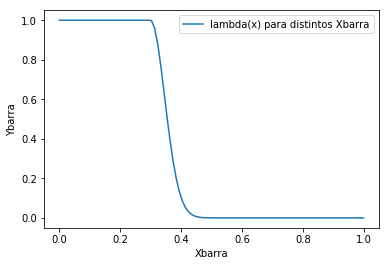
\includegraphics[scale=0.7]{img/LKratio.png}
    \caption{$lambda(x)$ en función de $\bar{x}$}
    \label{fig:lk_ratio}
\end{figure}
Donde ahora rechazaremos si $\lambda(x)\leq C$, pero, ¿cómo elegimos $C$?

Recordemos que queremos que el test sea de nivel $\alpha$, es decir, 
\begin{equation}
 	\sup_{\theta\in\Theta_0} \Probt{\lambda(x)\leq C} = \alpha
 \end{equation} 
 donde recordemos que $\lambda(x)$ es una función decreciente de $\bar{x}$, por lo que la condición $\lambda(x)\leq C$ puede expresarse como $\bar{x}\geq C'$, para algún $C'$. Esta expresión dependerá de $C'$, que es función de $C$, de $\theta_0$ y de $\alpha$; despejamos para $C$.

 \end{example} 
 \section{Test Chi cuadrado} 


 \section{Test de Kolmogorov-Smirnov} 
\label{sub:test_KS}

Ahora consideramos otro enfoque, basado en una estrategia muy distinta, al problema de test de hipótesis anterior para distribuciones no paramétricas:
	\begin{equation}
		H_0:F=F_0\quad \text{v.s.}\quad H_1:F\neq F_0.
	\end{equation}
En vez de discretizar, podemos construir la distribución empírica dada por 
\begin{equation}
	F_n(x) = \frac{1}{n}\sum_{i=1}^n\ind_{x_j\leq x}, 
\end{equation}
la cual realmente es una distribución (discontinua). 

Sabemos que, debido a la ley de los grandes números, 
\begin{equation}
	F_n(x)\to \E{\ind_{X\leq x}} = \Prob{X\leq x} =  F(x),
\end{equation}
además, por el teorema de Glivenko-Cantelli, tenemos 
\begin{equation}
	\sup_x|F_n(x)-F(x)| \to 0 \quad\text{c.s.}
\end{equation}
Lo anterior nos permite definir el estadístico  $D_n = \sup_x|F_n(x)-F_0(x)|$ y la región crítica
\begin{equation}
	R = \{x|D_n\geq k_\alpha\},
\end{equation}
donde $k_\alpha$ se elige imponiendo $\Probtz{D_n\geq  k_\alpha}=\alpha$.

\begin{remark}
El test de  Kolmogorov-Smirnoff sirve tanto para verificar si una VA sigue una distribución dada o si bien dos distribuciones siguen la misma distribución (desconocida).
\end{remark}

 \section{Test de Wilcoxon} 
\label{sub:test_Wilc}

Este es otro testo no paramétrico para verificar si dos VAs siguen la misma distribución. Consideremos las observaciones 
\begin{equation}
	X_1,\ldots,X_n\sim F,\quad Y_1,\ldots,Y_n\sim G,
\end{equation}
donde $F$ y $G$ son dos distribuciones, de las cuales solo sabemos que son continuas. 

Consideremos el siguiente problema de test de hipótesis: 
	\begin{equation}
		H_0:F=G\quad \text{v.s.}\quad H_1:F\neq G.
	\end{equation}
El test de Wilcoxon se enfoca en este escenario pero solo es sensible a diferentes \emph{localizaciones}, es decir, si $G$ es una versión desplazada de $F$.

Antes de ver el test de Wilcoxon, notemos que si nos interesase detectar estas desviaciones, entonces podríamos considerar un test que rechace $H_0$ si $|\bar{X} - \bar{Y}|\geq K$. Esto  es exactamente lo que hace el TRV en el problema 
	\begin{equation}
		H_0:\mu =  \eta \quad \text{v.s.}\quad H_1:\mu\neq \eta,
	\end{equation}
cuando $X\sim\cN(\mu,\sigma^2)$,  $Y\sim\cN(\eta,\sigma^2)$.

Sin embargo, en el caso general (cuando no sabemos nada de $F$) obtener la ley de $|\bar{X} - \bar{Y}|$ bajo $H_0$ no es trivial, lo cual es necesario para $\Probtz{|\bar{X} - \bar{Y}|\geq K} = \alpha$. En esta situación, el test de Wilcoxon propone considerar la siguiente observación conjunta 
\begin{equation}
	(z_1,\ldots,z_{m+n}) = (x_1,\ldots,x_n,y_1,\ldots,y_m),
\end{equation}
para luego considerar la secuencia ordenada de valores $z_i$ dados por 
\begin{equation}
	\min_i\{z_i\} = z_{(1)}\leq z_{(2)}\leq\cdots\leq z_{(n+m)} = \max_i\{z_i\}.
\end{equation}

Ahora podemos definir el concepto de \emph{rango} como la posición en el orden anterior, es decir, donde el rango de $z_{(1)}$ es 1, el rango de $z_{(2)}$ es dos  y así sucesivamente. 

\todo[inline]{dibujo de bolas negras y blancas.}

Denotando el rango de $x_i$ como $R_i$, podemos construir el estadístico
\begin{equation}
 	W = \sum_{i=1}^{n}R_i,
 \end{equation} 
esta cantidad debe intuitivamente interpretarse como el promedio de los rangos (es decir de la posiciones) que toman las observaciones de la variable $X$, por rechazamos $H_0$ si $W$ es muy pequeño o muy grande, es decir, si las muestras de $X$ no quedan \emph{mezcladas} con las de $Y$. 

 Esto es posible por que la distribución de $W$ bajo $H_0$ puede ser calculada y de hecho no depende de $F$, esto es porque (bajo $H_0$) los elementos de $z_i$ son iid, con lo que todas las posible permutaciones del los valores $z_i$ tienen la misma probabilidad dada por $\binom{n+m}{n}$.

 \begin{remark}[¿Cómo obtenemos la región crítica $R$ para este test?]
 	Podemos proceder de forma iterativa: Asumimos $H_0$, consideramos $R=\emptyset$ y agregamos las configuraciones de bolitas que tienen el menor y mayor valor de $W$, luego seguimos con las siguientes configuraciones hasta acumular una probabilidad $\Probtz{W\in\R} = \alpha$.
 \end{remark}
 
 \section{Test de Hipótesis Bayesiano}
 Hasta ahora sólo hemos visto los distintos test de hipótesis desde una perspectiva frecuentista. En todos estos test, había una relación asimétrica entre dos hipótesis: la hipótesis nula $H_0$ y la hipótesis alternativa $H_1$. Un proceso de desición se lleva acabo, y luego, en base a los datos observados, la hipótesis nula se va a rechazar a favor de $H_1$, o se aceptará. \\
 En el test de hipótesis Bayesiano, puede haber más de dos hipótesis en consideración, y no deben tener, necesariamente, una relación asimétrica.
 Para simplificar el análisis, consideremos dos hipótesis: $H_1$ y $H_2$.\\
 Sabemos que en algún momento tendremos datos $X$, sin embargo, aún no los tenemos. Nos interesa calcular las distribuciones posteriores $P(H_1|X)$ y $P(H_2|X)$. Usando Bayes: 
 $$
 P(H_1|X)=\dfrac{P(X|H1)P(H_1)}{P(X)} \text{ ; }
 P(H_2|X)=1-P(H_1|X)
 $$
Por probabilidades totales: 
$$
P(X)=P(X|H_1)P(H_1)+P(X|H_2)P(H_2)
$$
\begin{example}
    Consideremos un lanzamiento de una moneda, y las hipótesis: $H_1=$"La moneda no está cargada" ($\theta=\frac{1}{2}$) y $H_2$="La moneda no está cargada". Entonces, si $\theta$ es la probabilidad de que salga cara(C):
    $$
    P(\theta|H_1)=1_{\theta=0.5}
    $$
    Esto es una distribución a priori. Por otra parte, la hipótesis 2 es la que indica que la moneda está cargada. Consideremos que si la moneda está cargada, $\theta$ puede valer $1/3$ o $2/3$ de forma igualmente probable: 
     $$
    P(\theta|H_2)= 0.5 *1_{\theta=\frac{1}{3}} + 0.5* 1_{\theta=\frac{2}{3}}
    $$
    Por último, necesitamos las probabilidades $P(H_1)$ y $P(H_2)$. Consideremos (como se suele hacer) que $P(H_1)=P(H_2)=0.5$. Supongamos que al lanzar la moneda obtenemos la secuencia: CCSCSC. Entonces: 
    $$
    P(X|H_1)=  \binom{6}{4} (\dfrac{1}{2})^{4}(\dfrac{1}{2})^{2} =  \binom{6}{4} 0.0156 
    $$
    $$
    P(X|H_2) = P(X|\theta=1/3)P(\theta=1/3)+  P(X|\theta=2/3)P(\theta=2/3) =\binom{6}{4} 0.0137 
    $$
    Con los dos cálculos anteriores: 
    $$
    P(X)= \binom{6}{4} 0.0156 P(H_1) + \binom{6}{4} 0.0137 P(H_2) = \binom{6}{4} 0.01465
    $$
    Entonces: 
    $$
    P(H_1|X)=\dfrac{ \binom{6}{4} 0.0156 P(H_1)}{\binom{6}{4} 0.01465}  = 0.53
    $$
    Luego pasamos de $P(H_1)=0.5$ a $P(H_1|X)=0.53$, es decir, actualizamos nuestras creencias y ahora pensamos que es más probable que la moneda no esté cargada.
\end{example}
 
 En el test bayesiano, el ratio entre las verosimilitudes se llama \textbf{factor de bayes}.

\chapter{Regresión}
La palabra \emph{regresión} fue introducida por Francis Galton (1822-1911), haciendo referencia a que los hijos de personas altas, tendían a ser más bajos que sus padres,  fenómeno que denominó \textbf{Regresión a la media}. Este mismo fenómeno se puede observar cuando la segunda película de una saga no es tan buena como la primera parte. \\
La regresión es un método para estudiar la relación entre una variable $Y$, y otra variable independiente $X$, denominada característica. 
\begin{definition}[Función de Regresión] Se define la función de regresión $r(x)$ como:
$$
r(x)=\mathbb{E}(Y|X=x)=\int yf(y|x)dx
$$

\end{definition}
La idea de este método consiste en, dados datos $\mathcal{D}=\left \{ x_i,y_i \right \}_{i=1}^{n}$, encontrar una distribución $F_{X,Y}$. 
\section{Regresión Lineal Simple}
Comencemos viendo el caso unidimensional, es decir $X_i \in \R$. Buscamos ajustar $r(x)$ de forma tal que: 
$$
r(x)=\beta_0 + \beta_1 x,
$$

 es decir, de forma que y sea una función lineal (o lineal a fin ) de x. 
Supondremos que hay un ruido $\varepsilon_i$ tal que $\mathbb{V}(\varepsilon_i)=\sigma^2$, y es independiente de $x$. \\
\begin{definition}
Se define el modelo de regresión lineal simple como: 
$$
Y_i=\beta_0+\beta_1 X_i+ \varepsilon_i,
$$
con $\mathbb{E}(\varepsilon_i)=0$, y $\mathbb{V}(\varepsilon_i)=\sigma^2$.
\end{definition}
Buscamos estimar $\beta_0$ y $\beta_1$ de forma que tengamos una aproximación lineal que sea lo mejor posible. Estas últimas palabras nos hacen preguntarnos ¿Los mejores estimadores con respecto a qué? La respuesta es, con respecto a la métrica de mínimo cuadrados: 
$$
J(\hat{\beta_0},\hat{\beta_1})=\dfrac{1}{2} \sum_{i=1}^{n}(Y_i-\hat{Y_i})^{2},
$$
donde $\hat{Y_i}=\hat{\beta_0}+\hat{\beta_1}X_i$. 
\begin{theorem}
Los estimadores de mínimos cuadrados son: 
$$
\hat{\beta_1}=\dfrac{\sum_{i=1}^{n}(X_i-\bar{X})(Y_i-\bar{Y_i})}{\sum_{i=1}^{n}(X_i-\bar{X})^{2}}
$$
$$
\hat{\beta_0}=\bar{Y}-\hat{\beta_1}\bar{X}
$$
Un estimador insesgado de $\sigma^2$ es:
$$
\hat{\sigma^2}=\dfrac{1}{n-2} J(\hat{\beta_0},\hat{\beta_1})
$$
\end{theorem}
\section{Mínimos Cuadrados y Máxima Verosimilitud}
Supongamos ahora que $\varepsilon \sim \mathcal{N}(0,\sigma^2$, es decir, 
$Y_i|X_i \sim \mathcal{N}(\mu_i,\sigma^2)$, con $\mu_i=\beta_0 + \beta_1 X_i$.
Calculemos la verosimilitud: 
$$
\mathcal{L}=\prod_{i=1}^{n}f_{X}(X_i) f_{Y|X}(Y_i|X_i)= \prod_{i=1}^{n}f_{X}(X_i) \prod_{i=1}^{n}f_{Y|X}(Y_i|X_i)
$$
Llamemos $\mathcal{L}_1$ a la primera parte de este producto, y $\mathcal{L}_2$ a la segunda parte. Como $\mathcal{L}_1$ no depende de $\beta_0 $ y $\beta_1$, tenemos que para calcular los estimadores de máxima verosimilitud de estos parámetros, nos importa el segundo parámetro. Entonces, considerando la log-verosimilitud de $\mathcal{L}_2$:

$$ \mathcal{L}_2 = \prod_{i=1}^{n} f_{Y|X}(Y_i|X_i) \propto \sigma^{-n} exp(\dfrac{-1}{2\sigma^2}\sum_{i} (Y_i-\mu_i)^2) 
$$ 
$$
\implies l=-nlog(\sigma)-\dfrac{-1}{2\sigma^2}\sum_{i=1}^{n}(Y_i-(\beta_0 + \beta_1 X_i)^2
$$
Notemos que al minimizar esto, como el primer término es constante con respecto a $\beta_0 $ y $\beta_1$, tenemos: 
\begin{theorem}
Bajo la hipótesis de normalidad, el estimador de mínimos cuadrados coincide con el estimador de máxima verosimilitud. También se tiene: 
$$
\hat{\sigma}^2=\dfrac{1}{n} \sum_{i=1}^{n}(Y_i-\hat{Y_i})
$$
\end{theorem}
\begin{remark}
El estimador anterior de $\hat{\sigma}^2$ normalmente se reemplaza por el estimador insesgado de la parte anterior. 
\end{remark}

Lo anterior se puede extender al caso en que $X \in R^{k}$ de la siguiente forma. Suponemos: 
$$
Y_i= \sum_{j=1}^{k}\beta_j X_ij + \varepsilon_i,
$$
con $\mathbb{E}(\varepsilon_i)=0$. Denotemos:
$$
Y=\begin{pmatrix}
Y_1 \\
Y_2\\
.\\
.\\
.\\
Y_n\\
\end{pmatrix} ; 
X= \begin{pmatrix}
X_1 \\
X_2\\
.\\
.\\
.\\
X_n\\
\end{pmatrix}
$$
Cada fila de la matrix en $\R^{n \times k }$ $X$ es una observación. Sean:
$$
\beta= \begin{pmatrix}
\beta_1 \\
\beta_2\\
.\\
.\\
.\\
\beta_n\\
\end{pmatrix} \text{ y }
\varepsilon= \begin{pmatrix}
\varepsilon_1 \\
\varepsilon_2\\
.\\
.\\
.\\
\varepsilon_n\\
\end{pmatrix}
$$
Entonces: 
$$
Y=X\beta + \varepsilon
$$
\begin{theorem}
Si la matriz $X^{T}X$ es invertible: 
$$
\hat{\beta}= (X^{T}X)^{-1}X^{T}Y
$$
$$
\mathbb{V}(\hat{\beta})= \sigma^{2}(X^{T}X)^{-1}
$$
\end{theorem}

\begin{remark} Podemos tener observaciones de muchos $X_i$, pero no incluirlos todos al modelo. Un modelo más reducido tiene dos ventajas: La primera es que puede entregar mejores predicciones que un modelo más grande, y la segunda es que es más simple.\\  
Generalmente, mientras más variables se añaden a la regresión, el sesgo de la predicción disminuye pero aumenta la varianza. Una muestra pequeña genera mucho sesgo; esto se llama \emph{underfitting}. Una muestra muy grande lleva a una alta varianza; esto se llama \emph{overfitting}. Las buenas predicciones vienen de balancear sesgo y varianza. 
\end{remark}

\section{Regresión Logística}

\begin{definition}
Se llama función logística a la función: 
$$
f(x)=\dfrac{e^x}{1+e^x}
$$
\end{definition}
\begin{figure}[h]
    \centering
    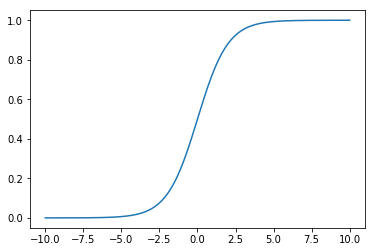
\includegraphics[scale=0.65]{img/funcion_logistica.png}
    \label{fig:logistica}
    \caption{Función Logística}
\end{figure}
La regresión logística es un método de regresión para el caso en que $Y_i \in \left \{0,1 \right \}$. El modelo considera: 

$$
p_i \equiv p_i(\beta) \equiv \mathbb{P}(Y_i=1 | X=x)= f(\beta_0+\sum_{j=1}^{k}\beta_{j} x_{ij}),
$$ 

con $f$ la función logística. De forma equivalente, si definimos $logit(p)=log(\dfrac{p}{1-p})$: 

$$
p_i=logit(p_i)= \beta_0+\sum_{j=1}^{k}\beta_j x_{ij}
$$

Como $Y_i$ son variables binarias, se tiene que   $Y_i|X_i=x_i \sim Ber(p_i)$. Así, la función de verosimilitud será:
$$
\mathcal{L}=\prod_{i=1}^{n} p_i(\beta)^{Y_i}(1-p_i(\beta))^{1-Y_i}
$$
Obtenemos el estimador de $\beta$, $\hat{\beta}$ usando método numéricos de optimización. 
\input{series_de_Tiempo}
\chapter{Markov Chain Monte Carlo}

Como hemos visto en los capítulos anteriores, con frecuencia el enfoque bayesiano implica calcular integrales que no son calculables con métodos convencionales, como el denominador cuando ocupamos Bayes, la marginalización de variables y el cálculo de esperanzas. También es necesario optimizar funciones que es muy difícil optimizar explícitamente, por ejemplo, al momento de maximizar la distribución posterior de un parámetro.  \\
Dados estos problemas, se hace natural buscar herramientas que nos permitan aproximar estas cantidades usando métodos numéricos, y con frecuencia, un computador. La herramienta que estudiaremos en esta sección, juega un rol fundamental en la integración, optimización, y también en la simulación de fenómenos físicos. 

\section{El principio de Monte Carlo}

La idea detrás de las simulaciones de Monte Carlo es extraer una muestra de observaciones i.i.d, $\mathcal{D}=\left \{ x_i \right \}_{i=1}^{N}$ de una densidad objetivo $p(x)$ desconocida. Las $N$ observaciones pueden usarse para aproximar la densidad objetivo de la forma: 
$$
p_{N}(x)=\dfrac{1}{N} \sum_{i=1}^{N} \delta_{x_i}(x)
$$
con $\delta_{x_i}(x)$ denota la delta de Dirac centrada en $x_i$. De esta forma, si buscamos aproximar la esperanza de $f$, $I(f)=\int f(x)p(x)$, lo haremos mediante las sumas: 
$$
I_{N}(f)= \dfrac{1}{N} \sum_{i=1}^{N}f(x_i) \overset{c.s}{ \underset{N \to \infty}{\rightarrow }} I(f)= \int f(x)p(x) 
$$
La convergencia anterior se cumple por la Ley de los Grandes Números Fuerte, e implica que $I_{N}(f)$ es un estimador insesgado. 






\chapter{Inferencia Causal} 

En este capítulo nos enfocaremos en métodos matemáticos que nos permitan modelar causas. Los métodos aquí presentados son bastante recientes, e intentan responder la pregunta \emph{"¿Cuándo $X$ causa $Y$?"}.\\
Estas dudas surgen de forma natural en un curso de estadística. Siempre se enseñan herramientas que permiten ver cuándo dos variables están asociadas, por ejemplo, con su correlación. Sin embargo, siempre se dice que \emph{"Asociación no implica causa"}. Es así como la estadística clásica respondió muchas veces la pregunta "¿Qué \textbf{no} es $X$ causa $Y$?", pero nunca "¿Qué es $X$ causa $Y$?". Esto fue así hasta que Judea Pearl introdujo la inferencia causal a finales del sigo pasado. Este trabajo logró que le dieran a Pearl un premio Turing, considerado el premio Nobel de ciencias de la computación, en el año 2011. \\
Informalmente, diremos que $X$ causa $Y$ si un cambio en el valor de $X$ cambia la distribución de $Y$. Podemos notar que cuando $X$ causa $Y$, $X$ e $Y$ están asociadas, pero la recíproca no es cierta. 

\section{El modelo contrafactual}

Sea $X$ una variable binaria, donde $X=1$ si $X$ "fue expuesta" y $X=0$, si $X$ "no fue expuesta". En este ámbito, la palabra "expuesta" puede referirse, por ejemplo, a que $X$ se expuso a un tratamiento médico, o a que $X$ realizó determinada acción. Por otro lado, sea $Y$ la variable resultado, por ejemplo, si hay o no una enfermedad. 

\definition Introducimos las variables aleatorias $C_0$ y $C_1$, llamadas resultados potenciales como: 
\begin{itemize}
    \item $C_0$ es el resultado si $X=0$
    \item $C_1$ es el resultado si $X=1$
\end{itemize}
Así: 
$$
Y=  \begin{cases}
      C_0, &  \text{ Si X =0} \\
		C_1, & \text{Si } X =1
    \end{cases}
$$

Esto se puede expresar como: 
$$
Y=C_{X}
$$
Lo anterior se llama la \textbf{Ecuación de Consistencia}. 
\begin{remark}
\begin{enumerate}
    \item Podemos pensar en $C_0$ y $C_1$ como variables escondidas que tienen toda la información relevante de un sujeto. 
    \item Si $X=0$, no observamos $C_1$. Luego decimos que $C_1$ es un contrafactual de $X=0$, pues es el resultado que hubiésemos obtenido si, contra los hechos (\emph{counter the facts}), $X=1. $
\end{enumerate}
\end{remark}

\definition Definimos el efecto causal promedio de $X$ sobre $Y$ por:
$$
\theta= \mathbb{E}(C_1)- \mathbb{E}(C_0)
$$

\begin{remark}
\begin{itemize}
    \item $\theta$ es el promedio si $X=1$ para todos, menos el promedio si $X=0$ para todos los sujetos.  
    \item $\theta$ mide el efecto causal de $X$. 
\end{itemize}
\end{remark}

\definition Se define la asociación de $X$ e $Y$ por: 
$$
\alpha= \mathbb{E}(Y|X=1)- \mathbb{E}(Y|X=0)
$$

\theorem En general, $\theta \not = \alpha$. (Asociación no implica causa). 
\example Queremos analizar el efecto que tiene una vitamina sobre una condición. Luego: 
$$
X= \begin{cases}
      1, &  \text{ Si la persona toma la vitamina} \\
		0, & \text{Si no }
    \end{cases}
$$
Por otra parte: 
$$
Y= \begin{cases}
      1, &  \text{ Si la persona está saludable} \\
		0, & \text{Si no }
    \end{cases}
$$
Observamos: 
\begin{center}
\begin{tabular}{cccc}
$X$ & $Y$ & $C_0$ & $C_1$ \\ \hline
$0$ & $0$ & $0$ & $0$* \\ 
$0$ & $0$ & $0$ & $0$* \\ 
$0$ & $0$ & $0$ & $0$* \\ 
$0$ & $0$ & $0$ & $0$* \\  \hline
$1$ & $1$ & $1$*& $1$ \\ 
$1$ & $1$ & $1$* & $1$ \\ 
$1$ & $1$ & $1$* & $1$ \\ 
$1$ & $1$ & $1$* & $1$ \\  
\end{tabular}
\end{center}

Los asteriscos hacen referencia a cantidades no observadas. Como $C_0=C_1$ para cada sujeto, tendremos: 
$$
\theta= \mathbb{E}(C_1)- \mathbb{E}(C_0)= \dfrac{1}{8} \sum_{i=1}^{8}C_{1,i}-\dfrac{1}{8} \sum_{i=1}^{8}C_{0,i}=0
$$
Luego el efecto causal promedio es $0$. Sin embargo, 
$$
\alpha= 1
$$

Luego $\theta \not = \alpha$. Sólo podemos concluir que la gente sana ($Y=1$) tiende a tomar la vitamina, mientras que la gente no sana, no.

En la mayoría de los casos, se hace difícil estimar $\theta$. Luego, se hace natural preguntarse cuando es posible dar un estimador para $\theta$. La respuesta es, cuando se hace una asignación aleatoria al tratamiento: 

\theorem Supongamos que asignamos el tratamiento al azar a los sujetos, y que $\mathbb{P}(X=0)>0$ y $\mathbb{P}(X=1)>0$. Entonces $\alpha = \theta$, y por lo tanto cualquier estimador consistente de $\alpha$ es un estimador consistente de $\theta$. 
En particular: 
$$
\hat{\theta}= \hat{\mathbb{E}}(Y|X=1)- \hat{\mathbb{E}}(Y|X=0) = \dfrac{1}{n_1} \sum_{i=1}^{n}Y_i X_i - \dfrac{1}{n_0} \sum_{i=1}^{n}Y_i (1-X_i),
$$
con $n_1= \sum_{i=1}^{n}X_i$ y $n_2=\sum_{i=1}^{n}1-X_i$. 

\textbf{Dem:} Como el tratamiento es asignado de forma aleatoria, tenemos que: 
$$
X \indep C_0, C_1
$$
Con esto: 
$$
\theta=\mathbb{E}(C_1)-\mathbb{E}(C_0) = \mathbb{E}(C_1|X=1) - \mathbb{E}(C_0|X=0) = \mathbb{E}(Y|X=1) - \mathbb{E}(Y|X=0) = \alpha \blacksquare
$$ 

\section{El modelo contrafactual: Generalización}
En la sección anterior se estudió que sucedía en el caso binario, es decir, el sujeto podía estar expuesto o no expuesto. Sin embargo, esta es una sobre simplificación de la realidad. Por ejemplo, si se desea estudiar el efecto de un medicamento sobre una enfermedad, no sólo será importante para el modelo si un sujeto se expuso o no a un medicamento, sino también cuál fue la dosis que tomaron. \\
Sea $x \in \mathcal{X}$. El vector $(C_0,C_1)$ pasará a ser la  \textit{función contrafactual} $C(x)$. Luego, en el ejemplo del medicamento $x$ será la dosis que tomó un sujeto, y $C(x)$ será el resultado que habría tenido un sujeto si hubiese recibido una dosis $x$. \\
Con lo anterior, la ecuación de consistencia se transforma en: 
$$
Y=C(X)
$$
Por otro lado, cambiamos el efecto causal promedio de $X$ sobre $Y$ por la función de regresión causal: 
$$
\theta(x)= \mathbb{E}(C(X)).
$$
Por otra parte la asociación se mide por la función de regresión: 
$$
r(x)=\mathbb{E}(Y|X=x)
$$

\theorem En general, $\theta(x) \not = r(x)$. Sin embargo, si X es asignado al azar (por ejemplo, por una prueba controlada aleatorizada), entonces $\theta(x)=r(x)$. 

Lamentablemente, dadas las dificultades que podría significar, la exposición de $X$ no suele ser al azar. Luego, ¿Cómo separamos aquello que podemos controlar para estudiar causalidad, y aquello que no?

\section{Confounders}

El problema que presenta que la exposición de $X$ no sea aleatoria es que genera que $C(X)$ no sea independiente de $X$. Pero, ¿Qué pasaría si pudiésemos separar los sujetos en grupos de forma que $X$ y $C(X)$ fueran independientes dentro de los grupos?.\\
Si lo pensamos, lo anterior no es muy difícil. Por ejemplo si estudiamos el efecto de un tratamiento médico, podríamos separar a las personas en distintos grupos según su edad, género, hábitos, etc. Dentro de un mismo grupo, se hace razonable que $X$ y $C(X)$ sean independientes. Las variables que usamos para asignar los distintos grupos se llaman \textbf{confounders} o \textbf{factores de confusión}. Si denotamos por $Z$ a todas estas variables, entonces: 
$$
\left \{ C(x): x \in \mathcal{X} \right \} \indep X |Z.
$$

\theorem Si $\left \{C(x): x \in \mathcal{X} \right \} \indep X |Z $, entonces: 
\begin{equation}
    \theta(x)= \int \mathbb{E}(Y | X=x,Z=z) dF_{Z}(z)dz
\end{equation}

Si $\hat{r}(x,z)$ es un estimador consistente de la funcióon de regresión $\mathbb{E}(Y|X=x,Z=z)$, entonces un estimador consistent de $\theta(x)$ es: 
\begin{equation}
    \hat{\theta}(x)= \dfrac{1}{n} \sum_{i=1}^{n} \hat{r}(x,Z_i)
    \label{eq: EAT}
\end{equation}

\begin{remark}
\begin{enumerate}
    \item Si $r(x,z)=\beta_0 + \beta_1 x + \beta_2 z$ entonces: 
    $$
    \hat{\theta}(x)= \hat{\beta}_0 + \hat{\beta}_1 x + \hat{\beta}_2 z,
    $$
    donde $(\hat{\beta}_0, \hat{\beta}_1, \hat{\beta}_2)$ son los estimadores de MCO. 
    \item Los epidemiólogos suelen llamar a la expresión de la ecuación \ref{eq: EAT} efecto ajustado de tratamiento. 
    \item La selección de factores de confusión \textbf{requiere} conocimiento experto. No es posible asegurarse de que no haya confounders que no conozcamos. 
    
\end{enumerate}
\end{remark}

Esta última observación tiene un efecto muy potente en la "filosofía" de la inteligencia artificial y en particular en el aprendizaje de máquinas según Judea Pearl. No es posible hacer que una máquina entienda relaciones causales sin un modelo con conocimiento humano experto. Pasar a ese nivel de "inteligencia" requiere que un humano haya modelado el fenómeno estudiado. 

\section{DAGs}

\definition Sean $X, Y,Z$ variables aleatorias. $X$ e $Y$ se dicen condicionalmente independientes dado $Z$ si: 
$$
f_{X,Y|Z}(x,y|z)= f_{X|Z}(x|z) f_{Y|Z}(y|z)\forall x,y,z  
$$
Esta relación se denota $X \indep Y |Z $.

\definition Un grafo dirigido $G$ es un par $(V,E)$, donde $V$ corresponde a los vértices, y $E$ a pares ordenados de vértices. 

Si se considera cada vértice en un grafo dirigido como una variable aleatoria, entonces esta se convierte en una forma muy conveniente de indicar independencia de las distintas variables. Para comprender este método, se hacen necesarias algunas definiciones y conceptos de Teoría de Grafos. 

\definition \begin{itemize}
    \item Si $\exists e \in E$ tal que $e=(X,Y)$, $X $ e $Y$ se dicen adyacentes. 
    \item  Si $\exists e \in E$ tal que $e=(X,Y)$, es decir el grafo tiene la configuración $X \rightarrow Y$ , se dice que $X$ es padre de $Y$, y que $Y$ es hijo de $X$. Se denota por $\pi_X$ o $\pi(X)$ al conjunto de padres de $X$.
    \item Un camino dirigido entre dos variables aleatorias es un conjunto de flechas apuntando en la misma dirección que va dese una variable a la otra. 
    \item $X$ es ancestro de $Y$ si existe un $X,Y$-camino dirigido. En este caso, $Y$ se dice descendiente de $X$. 
\end{itemize}

Esto nos permite graficar distintos tipos de relaciones causales e independencia entre variables. \\

\textbf{Insertar Dibujo}

\definition Una configuración de la forma $X \rightarrow Y \leftarrow Z $ se llama \textbf{collider}. Cualquier otra configuración se llama \textbf{no-collider}. 

Un camino dirigido se dice ciclo si empieza hay termina en el mismo vértice. Un grafo dirigido se dice acíclico si no contiene ciclos. De ahora en adelante, sólo trabajaremos con grafos dirigidos acíclicos o \textbf{DAGs} por su sigla en inglés (Directed Acyclic Graph).  

Si bien hoy en día el uso de DAGs como herramienta es bastante más común que hace un par de décadas, se debe tener en cuenta que fue muy difícil que la escuela clásica de la estadística lograra aceptarlos como una herramienta útil. Es más, no fueron los matemáticos ni los estadísticos los qu comenzaron usando esta herramienta, sino los epidemiólogos.  \\

\definition Sea $G=(V,E)$ un DAG, y sea $\mathbb{P}$ una distribución para $V$ con función de probabilidad $f$. Se dice que $G$ representa a $\mathbb{P}$ si: 
$$
f(v)=\prod_{i=1}^{k} f(x_i|\pi_i) 
$$
con $\pi_i$ padres de $x_i$. Se denota por $M(G)$ al conjunto de distribuciones representadas por $G$. 

\example \textbf{[insertar dibujo]} $\text{Sobrepeso} \rightarrow \text{Enfermedades al Corazón} \leftarrow \text{Fumar} \rightarrow \text{Tos} $

Tenemos que las enfermedades al corazón son un collider en el camino $ \text{Sobrepeso} \rightarrow \text{Enfermedades al Corazón} \leftarrow \text{Fumar}$. Además: 
$$
f(\text{Sobrepeso},\text{Enfermedades al Corazón}, \text{Fumar},\text{Tos})= 
$$

$$
f(\text{Sobrepeso}) f(\text{Fumar}) f(\text{Enfermedades al Corazón}|\text{Sobrepeso},\text{Fumar}) f(\text{Tos}|\text{Fumar}) 
$$

\theorem Dado $G=(V,E)$ un DAG, $\mathbb{P} \in M(G)$ si y sólo si $\forall W $ variable aleatoria, $W \indep \tilde{W}$

%agregar partes usando comando "input", el "\chapter" debe estar dentro del archivo a incluir




\end{document}

